\documentclass[11pt, a4paper]{memoir}
\usepackage[english, science, dropcaps, hyperref, submissionstatement]{ku-frontpage}
\usepackage[utf8]{inputenc}



\usepackage{pdfpages}
\usepackage{mathrsfs}
\usepackage{amsfonts}
\usepackage{amsmath}
\usepackage{mathtools}
\DeclareMathOperator\arctanh{arctanh}
\usepackage{amssymb}
\usepackage{bbm}
\usepackage{amsthm}
\usepackage{graphicx}
\usepackage{centernot}
\usepackage{caption}
\usepackage{subcaption}
\usepackage{braket}
\usepackage{lastpage}
\usepackage{enumitem}
\DisemulatePackage{setspace}
\usepackage{setspace}
\usepackage{xcolor}
\usepackage[english]{babel} 
\usepackage{dsfont}
\usepackage{appendix}
\usepackage{makecell}

\usepackage{tikz}
\usetikzlibrary{decorations.pathreplacing}
\newcommand{\tikznode}[3][inner sep=0pt]{\tikz[remember
	picture,baseline=(#2.base)]{\node(#2)[#1]{$#3$};}}
\usepackage{ytableau}

%\usepackage[T1]{fontenc}
%\usepackage{kpfonts}%  for math    
%\usepackage{libertine}%  serif and sans serif
%\usepackage[scaled=0.85]{beramono}%% mono


%\usepackage[sectionbib]{natbib}
\usepackage[square,sort,comma,numbers]{natbib}
%\usepackage[colorlinks=true,allcolors=blue]{hyperref}
%\usepackage[sectionbib]{bibunits}
%\defaultbibliographystyle{alpha}
%\defaultbibliography{bibliography}

\usepackage{fancyhdr}

\newcommand{\euler}[1]{\text{e}^{#1}}
\newcommand{\Real}{\text{Re}}
\newcommand{\Imag}{\text{Im}}
\newcommand{\supp}{\text{supp}}
\newcommand{\norm}[1]{\left\lVert #1 \right\rVert}
\newcommand{\abs}[1]{\left\lvert #1 \right\rvert}
\newcommand{\floor}[1]{\left\lfloor #1 \right\rfloor}
\newcommand{\ceil}[1]{\left\lceil #1 \right\rceil}
\newcommand{\Span}[1]{\text{span}\left(#1\right)}
\newcommand{\dom}[1]{\mathcal D\left(#1\right)}
\newcommand{\Ran}[1]{\text{Ran}\left(#1\right)}
\newcommand{\conv}[1]{\text{co}\left\{#1\right\}}
\newcommand{\Ext}[1]{\text{Ext}\left\{#1\right\}}
\newcommand{\vertin}{\rotatebox[origin=c]{-90}{$\in$}}
\newcommand{\interior}[1]{%
	{\kern0pt#1}^{\mathrm{o}}%
}
\renewcommand{\braket}[1]{\left\langle#1\right\rangle}
\newcommand{\ketbra}[2]{\left\vert #1\middle\rangle\middle\langle #2 \right\vert}
\newcommand*\diff{\mathop{}\!\mathrm{d}}
\newcommand{\ie}{i.e. }
\newcommand{\eg}{e.g. }
\newcommand{\dd}{\partial }
\newcommand{\R}{\mathbb{R}}
\newcommand{\C}{\mathbb{C}}
\newcommand{\w}{\mathsf{w}}
\newcommand{\rr}{\mathcal{R}}


\newcommand{\Gliminf}{\Gamma\text{-}\liminf}
\newcommand{\Glimsup}{\Gamma\text{-}\limsup}
\newcommand{\Glim}{\Gamma\text{-}\lim}

\newtheorem{theorem}{Theorem}[chapter]
\newtheorem{definition}[theorem]{Definition}
\newtheorem{proposition}[theorem]{Proposition}
\newtheorem{lemma}[theorem]{Lemma}
\newtheorem{corollary}[theorem]{Corollary}
\newtheorem{remark}[theorem]{Remark}
\newtheorem{conjecture}[theorem]{Conjecture}
\newtheorem{example}[theorem]{Example}

\numberwithin{equation}{section}

%\linespread{1.3}
\onehalfspacing


\setlength\arraycolsep{2 pt}
\setcounter{tocdepth}{2}
\setcounter{secnumdepth}{0}

\assignment{PhD thesis}
\author{Johannes Agerskov}

% The following are only needed if the \author, \title, \subtitle, and \date
% commands are not patchable. See the readme for more information.
\frontpageauthor{Johannes Agerskov}
\frontpagetitle{One-dimensional Dilute Quantum Gases and Their Ground State Energies}
%\frontpagesubtitle{An intruiging subtitle}
\frontpagedate{Submitted: March 31, 2023}

\title{One-dimensional Dilute Quantum Gases and Their Ground State Energies}
\subtitle{}
\date{Submitted: March 31, 2023}
\advisor{Advisor: Jan Philip Solovej}
%\frontpageimage{example.png}

\kupdfsetup{One-dimensional Dilute Quantum Gases and Their Ground State Energies}{}{Johannes Agerskov}

\interfootnotelinepenalty=10000

\begin{document}
	%\bibliographyunit[\chapter]
	\frontmatter
\begingroup
  \fontencoding{T1}\fontfamily{LinuxLibertineT-OsF}\selectfont
  \maketitle
\endgroup
\null\thispagestyle{empty}
\\
\hspace*{-1cm}{\textbf{Johannes Agerskov}\\
\hspace*{-1cm}QMATH\\
\hspace*{-1cm}Department of Mathematical Sciences\\
\hspace*{-1cm}University of Copenhagen\\
\hspace*{-1cm}\href{mailto:johannes-as@math.ku.dk}{johannes-as@math.ku.dk}\\
\hspace*{-1cm}\href{mailto:johannespwt@hotmail.com}{johannespwt@hotmail.com}
\vspace{5cm}

\hspace*{-1cm}\hspace{-0.88cm} \begin{tabular}{ll}
	Date of submission &\qquad March 31, 2023\\
	Date of defense &\qquad  June 6, 2023\\
	Advisor &\qquad  \makecell[tl]{\textbf{Jan Philip Solovej}\\ \ University of Copenhagen, Copenhagen, Denmark}\\
	Assessment committee &\qquad \makecell[tl]{\textbf{Søren Fournais} (Chair)\\
		\ University of Copenhagen, Copenhagen, Denmark\\
		\ Aarhus University, Aarhus, Denmark\\
	\textbf{Simona Rota Nodari}\\
	\ Université Côte d'Azur\\
	\ Nice, France\\
\textbf{Marcello Porta}\\
\ Scuola Internazionale Superiore di Studi Avanzati\\
\ Trieste, Italy }
	
\end{tabular}



\newpage
\begin{abstract}
	 In this thesis, we study the ground state energy of one-dimensional dilute quantum systems with repulsive pair potentials. We review part of the general theory of many-body quantum mechanics. We then prove results describing conditions under which, we can associate a unique self-adjoint many-body Hamiltonian to certain repulsive pair-potential.\\
	 The point-interacting solvable models in one dimension, \ie the Lieb-Liniger and Yang-Gaudin models, are reviewed and certain results related to their ground state energy in the dilute limit are proved.\\
	 We proceed by proving a ground state energy expansion for the Bose gas. This is done by proving first an upper bound and next a matching lower bound. The ground state energy is found, up to next-to-leading order, to depend on the potential only through the scattering length. Thus the system exhibits universality similar to that observed for higher dimensional systems. Our result covers the well known results on the ground state energy of the Lieb-Liniger model in the Tonks-Girardeau (dilute) limit. However, our result allows for a very general class of potentials, including potential that differ significantly from the point interacting $ \delta $-potentials for example by having positive scattering length. As corollaries, we find similar result for spin polarized Fermi gases and gases with intermediate particle statistics, \ie anyons.\\
	 Finally we study the spin--$ 1/2 $ Fermi gas. Here we conjecture a ground state energy expansion based on the solvable models at hand. The upper bound from the bosonic case is generalized by realizing the spins, in a given trial state, to be described by an effective antiferromagnetic Heisenberg chain. Thereby, we prove an upper bound matching our conjecture. As corollaries, we find similar results for spin-$ 1/2 $ bosons and for fermions and particles with spatial symmetry with spin-dependent potentials. Furthermore, we generalize parts of the lower bound proof from the bosonic case, and prove in this case for spin--$ 1/2 $ fermions a lower bound related to the Lieb-Liniger-Heisenberg ground state energy. We notice that for spin-dependent potentials in certain regimes identified with a ferromagnetic phase, the lower bound is reduced to that of the Lieb-Liniger model. Thus a lower bound, matching the previous upper bound, is proved in the ferromagnetic phase for spin-dependent potentials. 
\end{abstract}
\newpage
\renewcommand*\abstractname{Resumé}
\begin{abstract}
	I denne afhandling studerer vi grundtilstandsenergien af endimensionelle fortyndede kvantegasser med frastødende parpotentialer. Vi opsummerer dele af den generelle teori omkring mangelegemekvantemekanik. Derefter beviser vi under hvilket betingelser en unik selvadjungeret mangelegeme Hamilton-operator kan associeres til et givet parpotentiale. De punktinteragerende løsbare modeller i én dimension, dvs. Lieb-Liniger og Yang-Gaudin modellerne, opsummeres og visse resultater relateret til deres grundtilstandsenergi i den fortyndede grænse bevises.\\
	Vi forsætter ved at bevise en udvikling af grundtilstandsenergien for Bose-gassen. Dette gøres ved at vise først en øvre begrænsning og derefter en matchende nedre begrænsning. Det vises at grundtilstandsenergien, til næstledende orden, kun afhænger af potentialet igennem spredningslængden. Dermed udviser systemet universalitet, som ligner den observeret i tilsvarende højeredimensionelle systemer. Vores resultat dækker det velkendte resultat vedrørende grundtilstandenergien af Lieb-Liniger modellen i Tonks-Girardeau grænsen, altså den fortyndede grænse. Dog holder vores resultat for mere generelle parpotentialer, inklusiv potentialer der afviger markant fra $ \delta $-potentialer ekspemelvis ved at have positiv spredningslængde. Som korollarer finder vi lignende resultater for den spin-polariserede Fermi-gas og gasser med mellemliggende partikelstatistikker, altså anyoner.\\
	Endeligt studederer vi spin--$ 1/2 $ Fermi-gassen. Her præsenterer vi, som en formodning, en udvikling af grundtilstandsenergien baseret på kendte løsbare modeller. Den øvre begrænsning fra det bosoniske tilfælde generaliseres ved at indse, at partiklernes spin, i en givet variationsbølgefunktion, kan beskrives ved en effektiv antiferromagnetisk Heisenberg-kæde. Dermed beviser vi en øvre begrænsning, der tilsvarer den fremsatte formodning. Som korollarer finder vi lignende resultater for spin--$ 1/2 $ bosoner og for fermioner og partikler med rumlig symmetri med spin-afhængige potentialer. Ydermere generaliserer vi dele af beviset for den nedre begrænsning fra det bosoniske tilfælde, og vi beviser i dette tilfælde en nedre begrænsning for spin--$ 1/2 $ fermioner, der relaterer grundtilstandsenergien til dén fra Lieb-Liniger-Heisenberg modellen. Vi bemærker, at for spin-afhængige potentialer i visse regimer, som vi identificerer med en ferromagnetisk fase, reducerer den nedre begrænsing til dén af Lieb-Liniger modellen. Dermed bevises en nedre begrænsning, der matcher den førviste øvre begrænsning i netop den ferromagnetiske fase for spin-afhængige potentialer.
\end{abstract}

\newpage
\renewcommand*\abstractname{Acknowledgements}
\begin{abstract}
	As my time as a PhD student is coming to an end, there are many people to whom I am grateful. First and foremost, I would like to thank my advisor, Jan Philip Solovej, for introducing me to the field of dilute quantum gases, his exceptional advice, a good collaboration, and many interesting and very enjoyable discussions. It has been a pleasure being his student over the last three and a half years.\\
	I would also like to express my gratitude to Robin Reuvers for a good collaboration and many interesting and enjoyable discussions.\\
	Next, I would like to thank all of the members of QMATH over the last three and a half years for the good company both in and outside of the office. Special thanks go to Mads, Marie, Jacob, and August for being great coffee break buddies and for discussing a wide variety of subjects that includes, but does not restrict to, mathematics and physics.\\
	Also many thanks to Jacob Fronk and Lukas Junge for giving feedback on parts of this thesis.\\
	I am grateful to Robert Seiringer for valuable discussions during my visit to IST Austria and to IST Austria for the hospitality.\\
	I also thank my family, and my dad in particular, for all the encouragement, and my son for making me smile and laugh so very often.\\
	Finally, no one deserves my gratitude more than my fiancée, Martina, who has been ever supportive, through thick and thin, for the last almost ten years.
\end{abstract}
\renewcommand*\abstractname{Abstract}


\newpage
\tableofcontents
\newpage
\begin{center}
\large{\textbf{Preprint Included as Part of This Thesis}}\\
\normalsize

\begin{itemize}
\item[\cite{agerskov2022ground}]	Ground state energy of dilute Bose gases in 1D,\\
	 	\emph{Johannes Agerskov, Robin Reuvers, and Jan Philip Solovej,\\
	 	ArXiv, arXiv:2203.17183}\\
 	\footnotesize{\textbf{This preprint was revised and edited before being included in this thesis.}}
 	\normalsize
\end{itemize}
\end{center}

\mainmatter
 \chapter{Introduction}
Since the seminal work of Lee, Huang, and Yang in 1957 \cite{lee1957eigenvalues, lee1957many, huang1957quantum}, there has been a tremendous interest in dilute quantum gases and their ground state energy expansions. Finding good approximations for the bosonic ground state energy, at least in two and three dimensions, is intimately related to understanding the formation of Bose-Einstein condensates. Furthermore, such ground state energy expansions often exhibit universality. More specifically, the ground state energy of dilute systems tends to depend on the interaction potential only through the scattering length. This interest has in the mathematical physics literature grown during the last decades culminating in the recent completion of a rigorous proof of the Lee-Huang-Yang formula in 2019 \cite{yau2009second,fournais2020energy}\footnote{While the lower bound was made fully general in terms of assumptions on the interaction potential in 2021 \cite{fournais2021energy}, weakening the assumptions under which the upper bound can be proven is still an active field of research. }. With the problem essentially solved for the three dimensional Bose gas, it is natural to seek similar ground state energy expansions in other dimensions or with different particle statistics. Recently, the two dimensional bosonic ground state energy expansion was proven to analogous precision in \cite{fournais2022ground}, and previously the fermionic ground state energy expansions have been studied in both two and three dimensions \cite{lieb2005ground}.

The general one dimensional dilute Bose gas, or quantum gas in general, has been surprisingly little studied both in the physics and mathematics literature. This may be partly due to the presence of solvable models in one dimension. In 1963 Lieb and Liniger showed that the one dimensional Bose gas with point (delta-function) interactions is solvable by Bethe ansatz \cite{lieb1963exact}. In practice, this means that one may obtain algebraic equations for the ground state and excited energies, by realizing the eigenstates to be superpositions of plane waves with suitable scattering boundary conditions. Similarly, in 1967, the one dimensional spin--$ 1/2 $ Fermi gas with point interactions was shown, in the physics literature, to be solvable by means of a generalized Bethe ansatz \cite{yang1967some}. This argument was one year later further generalized to accommodate any symmetry of the domain and hence any spin \cite{sutherland1968further}. Some effort has since then gone into arguing that various confined three dimensional systems may be well approximated by such point interacting systems in one dimension, leaving the analysis of the spectrum already complete \cite{olshanii1998atomic,petrov2000regimes,dunjko2001bosons,lieb2003one,lieb2004one,seiringer2008lieb}. In \cite{lieb2003one,lieb2004one,seiringer2008lieb} it was shown that such an approximation indeed is valid in certain confinement regimes. We call this regime the \emph{weak confinement regime}, and it is described by having the trapping length scale, in the transverse direction much longer than the three dimensional scattering length scale. This means that transverse excitations cannot be neglected. On the other hand, one may instead consider the \emph{strong confinement regime}, described by having the transverse trapping length scale much shorter than the scattering length scale. In this regime, the spectrum will presumably be well described by a purely one dimensional system, with the three dimensional potential simply restricted to a line. A crucial difference in this case, is that the one dimensional scattering length arising from such confinements may be positive, as opposed to the effective Lieb-Liniger model in which the one dimensional scattering length always is negative.\\
In this thesis, we analyze ground state energies of general one dimensional dilute gasses. This covers the strongly point interacting models but further extends the result to models with positive scattering lengths. The ground state energy expansion for one dimensional dilute bosons and spin polarized fermions was recently obtained in \cite{agerskov2022ground}, which appears, in an edited version, as Chapter \ref{ChapterTheGroundStateEnergyOfTheOneDimensionalDiluteBoseGas} of this thesis. The expansion obtained will exhibit similar universality as in the three and two dimensional cases. However, one major difference is apparent in the analysis and phenomenology of the one dimensional gas: There is no Bose-Einstein condensation. This fact may be traced back to the celebrated theorem of Hohenberg, Mermin, and Wagner \cite{hohenberg1967existence,mermin1966absence}, which excludes longe-range order for one dimensional interacting systems. Thus the formation of a condensate is broken by the interaction in one dimension. This famous result is in agreement with the results found in this thesis, where we explicitly verify that the ground state energy shows greater similarity to energies arising from Slater determinant states than to energies arising from a condensate.\\
The proof of a ground state energy expansion for the one dimensional dilute Bose gas and spin polarized Fermi gas leaves the question of whether there is a similar expansion for the total ground state of the spin--$ 1/2 $ fermionic system. Such an expansion is conjectured in Chapter \ref{ChapterTheGroundStateEnergyOfTheOneDimensionalDiluteBoseGas} (\cite{agerskov2022ground}), based on the solvable models at hand for such a system. We present in Chapter \ref{ChapterTheGroundStateEnergyOfTheOneDimensionalDiluteSpin1/2FermiGas} a proof of an upper bound matching this conjecture. In the proof, we define a trial state in which the spin part is determined variationally. Interestingly, the variational problem determining the spin part is that of the one dimensional Heisenberg chain. In the case of the usual spin--$ 1/2 $ fermions, we get the antiferromagnetic Heisenberg chain. However, we will show that for models of a different symmetry or with spin-dependent potentials, the spin chain may be both ferro- or antiferromagnetic. Furthermore, we will present an idea of how to prove a corresponding lower bound. We do this by proving results that are analogous to findings of Chapter \ref{ChapterTheGroundStateEnergyOfTheOneDimensionalDiluteBoseGas} (\cite{agerskov2022ground}). However, it will be apparent that certain results do not generalize for the spin--$ 1/2 $ Fermi system straightforwardly. We then present a conjecture which, if proven true, allows us to complete the generalization of the Chapter \ref{ChapterTheGroundStateEnergyOfTheOneDimensionalDiluteBoseGas} results. We give heuristic arguments for the validity of this conjecture, but also highlight where these arguments are lacking in mathematical rigor. Finally, we notice that the result of Chapter \ref{ChapterTheGroundStateEnergyOfTheOneDimensionalDiluteBoseGas} do generalize for spin--$ 1/2 $ systems with other symmetries or spin-dependent potentials exactly when the system is in a ferromagnetic phase.\\

We summarize here overall the structure of this thesis: In Chapter \ref{ChapterMany-BodyQuantumMechanics}, we review relevant concepts in many-body quantum mechanics. Furthermore, since we will allow for quite general interactions in the later analysis, we review under which conditions on the interaction potential the dynamics of quantum systems can be defined in terms of a lower bounded self-adjoint Hamiltonian. We prove a result stating that in one dimension this is possible for any interaction potential that is the sum of a $ \sigma $-finite measure and an absolutely continuous measure. After this we review the concept of diluteness and known results about dilute quantum gases. Finally, we both review and prove certain result about two solvable models in one dimension. In Chapter \ref{ChapterTheGroundStateEnergyOfTheOneDimensionalDiluteBoseGas}, we find and prove ground state energy expansions for both the one dimensional Bose and spin polarized Fermi gas. In Chapter \ref{ChapterTheGroundStateEnergyOfTheOneDimensionalDiluteSpin1/2FermiGas}, we generalize some results from Chapter \ref{ChapterTheGroundStateEnergyOfTheOneDimensionalDiluteBoseGas} in order to prove an upper bound on the ground state energy of the one dimensional dilute spin--$ 1/2 $ Fermi gas. Furthermore, we generalize certain results related to the lower bound in Chapter \ref{ChapterTheGroundStateEnergyOfTheOneDimensionalDiluteBoseGas}. Finally, we notice that completing the proof of a lower bound for the spin--$ 1/2 $ Fermi gas, is possible by proving a conjecture on the ground state energy of a model known as the Lieb-Liniger-Heisenberg model in its antiferromagnetic phase. We also note, in the ferromagnetic phase, that a tight lower bound on the Lieb-Liniger-Heisenberg model is trivially valid. Thus for certain other symmetries or spin-dependent potential, we find a tight lower bound exactly when they are in a ferromagnetic phase in this sense.
In Chapter \ref{ChapterConclusionAndOutlook}, we give a final summary of our findings and discuss open problems.


% !TeX spellcheck = en_US
\chapter{Many-Body Quantum Mechanics}
	In this chapter we give a brief introduction to many-body quantum mechanics. The chapter will serve to define relevant quantities, to set up the mathematical framework, and to state some preliminary results.

\section{Many-body Wave Functions}
	In quantum mechanics a system is described by a \emph{state} or \emph{wave function} in an underlying Hilbert space. 
	\begin{definition}
		A quantum system at fixed time is a pair \begin{equation*}
			(\Psi,\mathcal{H}),\text{ with } \Psi\in\mathcal{H} \text{ and } \norm{\Psi}=1,
		\end{equation*}
		where $ \mathcal{H} $ is a Hilbert space. Here $ \Psi $ is called the state or wave function of the system.
	\end{definition}
	In this thesis, we are mostly interested in quantum system consisting of $ N $ particles in a region $ \Omega\subseteq \R^d $, possibly with spin degrees of freedom $ \{S_i\}_{i\in{1,\ldots,N}} $. We refer to $ d $ as the \emph{dimension} of the system. Such a system is described by having $$ \mathcal{H}= L^2\left(\prod_{i=1}^{N}\left(\Omega\times \{-S_i,...,S_i\}\right) \right)=\otimes_{i=1}^{N}L^2\left(\Omega;\C^{2S_i+1}\right), $$ where $ S_i $ is the \emph{spin} of the $ i $th particle. Since we are more specifically interested in identical particles we will further restrict the structure of the underlying Hilbert space below.

	\subsection{Identical Particles: Bosons and Fermions}
		In the case when the particles in question are identical, \ie indistinguishable, it turn out that one can restrict the underlying Hilbert space, to have certain symmetries. Considering $ N $ indistinguishable particles, we restrict to the physical configuration space to $ C_{p,N}=C_N/S_N $, with $ C_N:=\{(x_1,\ldots,x_N)\in \Omega^N \vert x_i\neq x_j \text{ if }i\neq j\} $ on which the symmetric group act freely. For $ d\geq 2 $, we then require the wave function of the system to take values in a unitary irreducible representation of the fundamental group $\pi_1(C_{p,N})$, where we noted that the physical configuration space is path-connected in order for $ \pi_1(C_{p,N},x) $ to be independent of $ x\in C_{p,N} $.
		\begin{remark}
			For $ d\geq 3 $ we have $\pi_1(C_{p,N})=S_N$, for $ d=2 $ we have $\pi_1(C_{p,N})=B_N$ and for $d=1$ we have $\pi_1(C_{p,N})=\{1\}$. In the somewhat special case of $d=1$, $C_{p,N}=\{x_1<x_2<\ldots<x_N\}$. On this configuration space one can never interchange particles without crossing the singular excluded incidence (hyper)planes. Thus the allowed particle statistics are determined by the possible permutation invariant dynamics (see section below) on this space. In section ... we will see examples of different particle statistics in one dimension. 
		\end{remark}
		\begin{remark}
			Adding spin to the above considerations amounts to having $C_N:=\{(z_1,\ldots,z_N)\in \left(\Omega\times\{-S,\ldots,S\}\right)^N \vert (z_i)_1\neq (z_j)_1 \text{ if }i\neq j\}$, and $C_{p,N}:=C_N/S_N$. In this case $C_{p,N}$ is not path connected, however, for each configuration of spins $ \sigma=(\sigma_1,\ldots,\sigma_N)\in\{-S,\ldots,S\}^N $ the configurations spaces $ C_{p,N,\sigma}=\{((x_1,\sigma_1),\ldots,(x_N,\sigma_N))\in \left(\Omega\times\{-S,\ldots,S\}\right)^N \vert x_i\neq x_j \text{ if }i\neq j\} $ are path connected and their fundamental groups are isomorphic to the fundamental group in the spinless case independent of $ \sigma $.\\
			Alternatively, one can view the wave function as a $ (2S+1)^N $-dimensional vector bundle over the physical (spinless) configuration space.
		\end{remark}
		In the remaining part of this thesis, we will mainly be interested in the two irreducible representations that are the symmetric representation and the anti-symmetric representation, in which we refer to the particles as \emph{bosons} and \emph{fermions} respectively. It is an empirical fact that bosons and fermions are the only types of elementary particles that are encountered in nature. Hence for bosons we restrict to wave functions in the symmetric (or bosonic) subspace $ L^2_{s}\left(\left(\Omega\times \{-S,\ldots,S\}\right)^N \right)\cong\vee_{i=1}^{N}L^2\left(\Omega; \C^{2S+1}\right)$ and for fermions we restrict to wave-functions in the anti-symmetric (or fermionic) subspace $ L^2_{a}\left(\left(\Omega\times \{-S,\ldots,S\}\right)^N \right)\cong\wedge_{i=1}^{N}L^2\left(\Omega; \C^{2S+1}\right)$.\\
		To recap we list the following important definitions
		\begin{definition}
			A quantum system of $N$ spin--$ S $ bosons in $ \Omega\subseteq\R^d $ at fixed time is a pair
			\begin{equation*}
			(\Psi,\mathcal{H}),\text{ with } \Psi\in\mathcal{H}\text{ and }\norm{\Psi}=1,
			\end{equation*}
			where $ \mathcal{H}=L^2_{s}\left(\left(\Omega\times \{-S,\ldots,S\}\right)^N \right)\cong\vee_{i=1}^{N}L^2\left(\Omega; \C^{2S+1}\right) $.
		\end{definition}
		\begin{definition}
			A quantum system of $N$ spin--$ S $ fermions in $ \Omega\subseteq\R^d $ at fixed time is a pair
			\begin{equation*}
			(\Psi,\mathcal{H}),\text{ with } \Psi\in\mathcal{H}\text{ and }\norm{\Psi}=1,
			\end{equation*}
			where $ \mathcal{H}=L^2_{a}\left(\left(\Omega\times \{-S,\ldots,S\}\right)^N \right)\cong\wedge_{i=1}^{N}L^2\left(\Omega; \C^{2S+1}\right) $.
		\end{definition}
	
\section{Observables, Dynamics, and Energy}
In general we call any self-adjoint operator on $ \mathcal{H} $ an \emph{observable}. Physically, observables represent quantities that, in principle, can be measured in an experiment. It is a postulate of quantum mechanics that given an observable $ \mathcal{O}=\int_{\sigma(\mathcal{O})}\lambda \diff P_\lambda $, where $\{P_\lambda\}_{\lambda\in\sigma(\mathcal{O})}$ is the projection valued measure associated to $ \mathcal{O} $ by the spectral theorem \cite{reed1981functional}, the probability of a measurement of $ \mathcal{O} $ in state $ \Psi\in\dom{\mathcal{O}} $ having outcome $ \lambda\in M\subset \R $ is given by $ P\left((\mathcal{O},\Psi)\rightarrow\lambda\in M\right)=\int_{\lambda\in M} \braket{\Psi,P_\lambda\Psi} $. 
Furhtermore we defined the expected value of an observable.
\begin{definition}
	The \textbf{expectation value} of an observable $ \mathcal{O} $ in state $ \Psi\in\dom{\mathcal{O}} $ is 
	$$ \braket{\mathcal{O}}_\Psi:=\int_{\lambda\in\sigma(\mathcal{O})}\lambda\braket{\Psi,P_\lambda\Psi} $$
	where $\{P_\lambda\}_{\lambda\in\sigma(\mathcal{O})}$ is the projection valued measure associated to $ \mathcal{O} $ by the spectral theorem.
\end{definition}


I the previous section we defined a quantum system at a fixed time. However, we are often interested in dynamics of the system. In quantum mechanics, time evolution is modeled by the infinitesimal generator of time evolution, $ H $, also known as the \emph{Hamiltonian}. We will in this thesis take $ H $ to be a (time-independent) lower bounded self-adjoint operator on $ \mathcal{H} $. A state evolves in time according to the Schr\"odinger equation\begin{equation*}
\Psi(t)=\exp\left(-iH(t-t_0)\right)\Psi(t_0),
\end{equation*}
where have set $ \hbar=1 $.
\begin{remark}
	By Stone's theorem (ref Reed and Simon), the existance of a self-adjoint Hamiltonian, $ H $, is guaranteed for any time evolution described by $ \Psi(t)=U(t-t_0)\Psi(t_0) $, when $ U(t) $ is a strongly continuous one-parameter unitary group.
\end{remark}
Since the Hamiltonian, $ H $, is self-adjoint, it represents an observable which we call \emph{energy}. Since $ H $ is lower bounded, there is a natural notion of lowest energy of $ H $.
\begin{definition}
	The \textbf{ground state energy} of $ H $ is defined by 
	$$
	E_0(H):=\inf(\sigma(H))
	$$
\end{definition}
Furthermore, we define the notion of a \emph{ground state} of $ H $ as
\begin{definition}
	We say that a (normalized) state $ \Psi\in \dom{H}\subset \mathcal{H} $ is a \textbf{ground state} of $ H $ if $$ \braket{H}_\Psi=E_0(H). $$
\end{definition}
When studying ground states and ground state energies it is useful to have the following variational characterization.
\begin{remark}\label{RemarkVariationalPrinciple1}
	It follows from the spectral theorem (ref Reed and Simon) that the ground state energy is given by \begin{equation}\label{EqVariationalGroundStateEnergyOperator}
		E_0(H)=\inf_{\Psi\in \dom{\mathcal{H}}}\frac{\braket{\Psi,H\Psi}}{\norm{\Psi}^2}.
	\end{equation}
\end{remark}
\begin{remark}
	It is straightforward to show that the quadratic form $ \dom{H}\ni\Psi\mapsto\braket{\Psi,H\Psi} $ is lower bounded and closable, since $ H $ is lower bounded and self-adjoint.
\end{remark}
\begin{definition}
	Given a Hamiltonian, $ H $, we define the \textbf{associated energy quadratic form}, $ \mathcal{E}_H:\mathcal{\dom{\mathcal{E}_H}}\to \R $, as the closure of the quadratic form $ \dom{H}\ni\Psi\mapsto\braket{\Psi,H\Psi} $. When $ H $ is given from the context, we will often write $ \mathcal{E} $ as short for $ \mathcal{E}_H $.
\end{definition}
\begin{remark}\label{RemarkVariationalPrinciple2}
	From the definition of $\mathcal{E_H}$ and from Remark \ref{RemarkVariationalPrinciple1} it follows straightforwardly that we have \begin{equation}\label{EqVariationalGroundStateEnergyForm}
		E_0(H)=\inf_{\Psi\in \dom{\mathcal{E_H}}}\frac{\mathcal{E_H}(\Psi)}{\abs{\Psi}^2}=\inf_{\substack{\Psi\in \dom{\mathcal{E_H}},\\\norm{\Psi}=1}}\mathcal{E_H}(\Psi), 
	\end{equation}
	as $ \dom{H} $ is form core for $\mathcal{E_H}$.
\end{remark}
We refer to both \eqref{EqVariationalGroundStateEnergyOperator} and \eqref{EqVariationalGroundStateEnergyForm} as \emph{the variational principle}.
We will often in the remaining take \eqref{EqVariationalGroundStateEnergyForm} as the vary definition of the ground state energy. Furthermore, one can also define the dynamics of a quantum system by specifying an energy quadratic form in the following sense
\begin{remark}[Ref!!]\label{RemarkOperatorFromQuadraticForm}
	Given a densely defined, lower bounded, closable, quadratic form $ \mathcal{E}:\dom{\mathcal{E}}\to \R $ there exist a \textbf{unique} lower bounded, self-adjoint operator $ H_\mathcal{E} $, such that $ \mathcal{E}(\Psi)=\braket{\Psi,H_\mathcal{E}\Psi} $ for all $ \Psi\in \dom{H_\mathcal{E}} $, and $ \dom{H_\mathcal{E}} $ is form core for $\overline{\mathcal{E}}$, \ie the form closure of $ \braket{\cdot,H_\mathcal{E}\cdot} $ is equal to the form closure of $\mathcal{E}$. 
\end{remark}
Thus we will frequently change between the two equivalent formulations of the dynamics of a quantum system that are the operator, $ H $, formulation and the quadratic form, $ \mathcal{E} $, formulation
\subsection{Many-Body Hamiltonians}
Until this point, we have not specified the class of Hamiltonians that we will be interested in. We have seen, that we will care mainly about Hamiltonians defined on the bosonic or fermionic subspace, however no specification has been made about the dynamics on these subspaces. We are interested in modeling $ N $ particles in some region $ \Omega\subseteq\R^d $ that interact locally with each other. For the remaining of this subsection we will ignore spin, knowing that including spin degrees of freedom is completely analogous. In practice, and for suitably mild interactions, this means that the Hamiltonian \emph{formally} (meaning restricted to the fermionic or bosonic subspace of $ C^\infty_0(\Omega^N) $) takes the form \begin{equation}
H=\sum_{i=1}^{N}T_i+U(x_1,\ldots,x_N)
\end{equation}
where $ T_i $ is the \emph{kinetic energy operator} for particle $ i $ and the \emph{potential} $ U $ is a multiplication operator which models the local interaction among the particles. The kinetic energy operator is taken to be\footnote{This is usually justified by going through a canonical quantization procedure for the classical Hamiltonian function of the system we are interested in modeling} \begin{equation}
T_i=-\frac{1}{2m_i}\Delta_i\qquad (\hbar=1)
\end{equation} 
since we interested in identical particles, we will from this point onward choose $ m_i=1/2 $. As for the potential, $ V $, we of course immediately restrict to permutation-invariant function, $ U $, for identical particles. However, in the following we will further restrict to a combination of having a trapping potential and radial pair potentials, which model pairwise interactions that only depend on the distances between particles. Such potentials take the form \begin{equation}
U(x_1,\ldots,x_N)=\sum_{i<j} v(x_i-x_j) + \sum_{i=1}^{N}V(x_i)
\end{equation}
where we take $ v $ to be a radial function and, $ V $, is called the \emph{trapping potential}. We will generally take $ v $ to be repulsive, meaning $ v\geq 0 $, with compact support. The trapping potential we will disregard \ie $ V=0 $. We will then in general take the true Hamiltonian to be a self-adjoint extensions of the symmetric \emph{formal} Hamiltonian. Now some models of stronger interactions, \eg the hard core interaction, requires a more delicate construction with respect to the initial definition of the formal Hamiltonian. However, the construction of the Hamiltonian can be done in a more unified manner when constructing the energy quadratic form. 
\begin{definition}
	For a system of $ N $ bosons/fermions in region $ \Omega\in\R^d $, we define for $ \sigma\in[0,\infty] $ \textbf{the energy quadratic forms}
\begin{equation}\label{key}
\mathcal{E}_{(v,\sigma)}(\Psi)=\int_{\Omega^N} \sum_{i=1}^{N}\abs{\nabla_i\Psi}^2+\sum_{i<j} v(x_i-x_j)\abs{\Psi}^2+\sigma\int_{\dd (\Omega^N)}\abs{\Psi}^2,
\end{equation}
with domain $ \dom{\mathcal{E}_{(v,\sigma)}}=\{\Psi\in (C^\infty_0(\Omega^N))_{\text{b/f}}\vert \mathcal{E}_{(v,\sigma)}(\Psi)<\infty\} $. with $ (C^\infty_0(\Omega^N))_{\text{b/f}} $ meaning the bosonic/fermionic subspace of $ C^\infty_0(\Omega^N) $. $ \sigma=\infty $ is taken to mean Dirichlet boundary conditions.
\end{definition}
Of course $ \mathcal{E}_{(v,\sigma)}\geq 0 $ for any $ \sigma\in[0,\infty] $ and $ v\geq 0 $. However, the closability of $ \mathcal{E}_{(v,\sigma)} $ is not evident. In fact for general $ v $, $ \mathcal{E}_{(v,\sigma)} $ will not be neither densely defined nor closable on $ L^2_{s/a}(\Omega^N) $. However, it will both densely defined on a closed subspace $ \mathcal{H}_{(v,\sigma)}:=\overline{\dom{\mathcal{E}_{(v,\sigma)}}}^{\norm{\cdot}_2} $ of $ L^2_{s/a}(\Omega^N) $, hence we take $ \mathcal{H}_{(v,\sigma)} $ to be the Hilbert space of the system, when this is the case. Closability of $ \mathcal{E}_{(v,\sigma)} $ on $ \mathcal{H}_{(v,\sigma)} $ is not necessarily satisfied. Thus we make the following definition
\begin{definition}
	We say a potential $ v\geq 0 $ is \textbf{allowed} in dimension $ d $, if $ \mathcal{E}_{(v,\sigma)} $ is closable on $ \mathcal{H}_{(v,\sigma)}:=\overline{\dom{\mathcal{E}_{(v,\sigma)}}}^{\norm{\cdot}_2}\subset L^2_{s/a}(\Omega^N)$ for any $ \sigma\in[0,\infty] $.
\end{definition}
\begin{remark}
	There are plenty of allowed potentials, but the notion does depend on the dimension, $ d $. For example is $ v=\delta_0 $, \ie the delta function potential, allowed in dimension $ d=1 $, but not in dimension $ d\geq 2 $. This can be seen from the fact that for $ d=1 $ the incidence planes are co-dimension $ 1 $, and hence the trace theorem gives closability, but for $ d\geq 2 $ where the incidence planes are of co-dimension $ \geq 2 $ it is known that the trace of $ H^1 $ is not contained in $ L^2 $. (Ref!!)
\end{remark}


\begin{remark} \label{RemarkdDimPotentialAllowed}
	For any radial $ v\geq 0 $ that is measurable  $\mathcal{E}_{(v,\sigma)} $ is the quadratic form associated to a self-adjoint operator on some Hilbert space $ \mathcal{H}_{(v,\sigma)}\subset L^2_{s/a}(\Omega^N) $. It is well known that $\mathcal{E}_{(0,\sigma)}$ is closable on $ \mathcal{H}_{(0,\sigma)}\supseteq \mathcal{H}_{(v,\sigma)}    $, hence on $  \mathcal{H}_{(v,\sigma)} $. Thus closability of $ \mathcal{E}_{(v,\sigma)} $ amount to showing that $ \psi_n \xrightarrow{\norm{\cdot}_2}0 $ as $ n\to\infty $ and $ (\psi_n)_{n\in\mathbb{N}}\subset L^2\left(\Omega^N,\underbrace{\sum_{i<j}v(x_i-x_j)\diff\lambda^{N}}_{\coloneqq \diff\mu_v}\right) $ Cauchy, implies $ \psi_n\xrightarrow{\norm{\cdot}_{L^2(\Omega^N,\diff\mu_v)}}0  $. This is evident from the fact that $\psi_n\xrightarrow{\norm{\cdot}_{L^2(\Omega^N,\diff\mu_v)}}f$ for some $ f\in L^2(\Omega^N,\diff\mu_v) $ by completeness. Now $ \psi_n $ has a subsequence that converges $ \lambda^{N} $--almost everywhere to $ 0 $, and this subsequence further has a subsequence that converges $ \mu_v $--almost everywhere to $ f $. Hence $ f=0 $ $ \mu_v $--almost everywhere, as $ \mu_v\ll \lambda^N $. \\
	Thus there is a corresponding self-adjoint operator $ H_{(v,\sigma)} $ to $ \mathcal{E}_{(v,\sigma)} $ on $ \mathcal{H}_{(v,\sigma)} $, which we shall formally write as $ H_{(v,\sigma)}=-\sum_{i=1}^{N}\Delta_i+\sum_{1\leq i<j\leq N}v(x_i-x_j) $.
\end{remark}
The argument from the previous may be generalized slightly in the case of $ d=1 $, in order to show that any $ \sigma $--finite measure $ v\diff\lambda^{N} $ is allowed as potential. Notice that we slightly abuse notation and write $ v(x_i-x_j)\diff\lambda^N $ even when $ v $ is a singular continuous measure and thus has no density. However, we do think of $ v $ a being a one-dimensional measure in the sense that 
$$ v(x_i-x_j)\diff\lambda^N:=\diff\mu_{v_{ij}}\times \diff \lambda^{N-1}_{(x_i-x_j)=\text{ fixed}},  $$ 
where we defined $ \diff \mu_{v_{ij}}:=v(x_i-x_j)\diff (x_i-x_j) $ and $ \lambda^{N-1}_{(x_i-x_j)=\text{ fixed}} $ to be the measure such that $ \diff\lambda^{N}=\diff(x_i-x_j)\times \diff\lambda^{N-1}_{(x_i-x_j)=\text{ fixed}} $. Uniqueness of the product measure is guaranteed by $ \sigma $-finiteness of $ v $.
%\begin{lemma}
%	Let $ (f_n)_{n\in\mathbb{N}}\subset H^1(\Omega) $ be a sequence such that $ \norm{f_n}_{H^1}\to0 $ as $ n\to\infty $. Then $ f_n $ has a subsequence that converges pointwise to 0 on $ \lambda^{N-1} $--almost all lines.
%\end{lemma}
%\begin{proof}
%	We pass to a subsequence, which we also denote $ f_n$, such that $ f_n $ converges pointwise $ \lambda^N $--a.e. to $ 0 $. 
%	Since $ f_n\in H^1(\Omega) $, we know that $ f_n $ are absolutely continuous on $ \lambda^{N-1} $--almost all lines. Now consider the $ H^1(\R) $ norms of $ f_n $ along each line. Clearly these constitute $ L^2 $ functions, with norms converging to $ 0 $. Hence there exist a subsequence that converges pointwise $ \lambda^{N-1} $--almost everywhere to $ 0 $. Thus there is a subsequence such that for almost all lines, the $ H^1 $ norm along the line converges to zero. But then $ f_n $ converges, by Morrey's inequality, uniformly to 0 on almost all lines.
%\end{proof}
%precise statement. 
We will need the following essential lemma, where we use the notation  $ \lambda_k^{N-1}\coloneqq \prod_{i\neq k}\diff x_i $ 
\begin{lemma}\label{LemmaH1PointwiseConvergence}
	Let $ (f_n)_{n\in\mathbb{N}}\subset H^1(\Omega^N) $ be a sequence such that $ \norm{f_n}_{H^1}\to0 $ as $ n\to\infty $. Then defining $ f^k_n(t,\overline{x}^k)\coloneqq f_n(x_1,\ldots,x_{k-1},t,x_{k+1},\ldots,x_N) $ for any $ k=1,\ldots,N $, we have that $ (f^k_n)_{n\in\mathbb{N}} $ has a subsequence that converges pointwise (in $ t $) to $ 0 $, $ \lambda_k^{N-1} $--a.e. for all $ k=1,\ldots,N $.
\end{lemma}
\begin{proof}
	We pass first to a subsequence, which we also denote $ f_n$, such that $ f_n $ converges pointwise $ \lambda^N $--a.e. to $ 0 $. 
	Since $ f_n\in H^1(\Omega^N) $, we know for any $ k=1,\ldots,N $ that $ f^k_n(t,\overline{x}^k) $ are in $ H^1(\Omega) $ (as functions of t) $ \lambda_k^{N-1} $--a.e.
	[\cite{evans1991measure} Theorem 2 p. 164].
	Now consider the $ H^1(\Omega) $ norms of $ g_n^k(\overline{x}^k)\coloneqq \norm{f^k_n(\cdot,\overline{x}^k)}_{H^1(\Omega)} $. Clearly $ g_n^k $ constitute $ L^2 $ functions, with norms converging to $ 0 $. Hence there exist a subsequence that converges pointwise $ \lambda_k^{N-1} $--almost everywhere to $ 0 $. Then there is a subsequence $ f_{n_i}^k $ such that for $ \lambda_k^{N-1} $--a.e. $ \overline{x}^k $, $ f_{n_i}^k(\cdot,\overline{x}^k) $ converges to $ 0 $ in $ H^1(\Omega) $. But then $  f_{n_i}^k(\cdot,\overline{x}^k) $ converges, by Morrey's inequality, pointwise to $ 0 $.
\end{proof}
Using this lemma, we may prove the following Proposition
\begin{proposition}\label{Lemma1dPotentialAllowed}
	Let $ d=1 $, then for any $ \sigma $-finite measure, $ v $, we have that $ \mathcal{E}_{(v,\sigma)} $ is the quadratic form associated to a self adjoint operator $ H_{(v,\sigma)} $ on some Hilbert space $ \mathcal{H}_{(v,\sigma)} $.
\end{proposition}
\begin{proof}
	As previously, we define $\mathcal{H}_{(v,\sigma)}:=\overline{\dom{\mathcal{E}_{(v,\sigma)}}}^{\norm{\cdot}_2} $ and $ \diff\mu_v=\sum_{1\leq i<j\leq N}v(x_i-x_j)\diff\lambda^N $. Clearly $ \mathcal{E}_{(v,\sigma)} $ is lower bounded and densely defined in $ \mathcal{H}_{(v,\sigma)} $. Closability amounts to showing that $ \psi_n\xrightarrow{\norm{\cdot}_{L^2(\Omega^N,\diff\lambda^{N})}}0 $ and $ (\psi_n)_{n\in\mathbb{N}}\subset L^2\left(\Omega^N,\diff\mu_v\right) $ Cauchy w.r.t the norm $ \norm{\cdot}_{\mathcal{E}_{(v,\sigma)}}=\sqrt{\mathcal{E}_{(v,\sigma)}(\cdot)+\norm{\cdot}_2^2} $, implies $ \psi_n\xrightarrow{\norm{\cdot}_{L^2(\Omega^N,\diff\mu_v)}}0  $. Now since $ (\psi_n)_{n\in\mathbb{N}}$ is a Cauchy sequence in $ L^2\left(\Omega^N,\diff\mu_v\right) $, it has a subsequence that converges $ \mu_v $--almost everywhere to some function $ f\in L^2\left(\Omega^N,\diff\mu_v\right)  $. Furthermore, this subsequence has a further subsequence that converges $ \lambda^{N} $--almost everywhere to $ 0 $. However, since $ (\psi_n)_{n\in\mathbb{N}}$ converges to $ 0 $ in $ H^1(\Omega^N,\diff \lambda^N) $, Lemma \ref{LemmaH1PointwiseConvergence} implies that for $ (x_i-x_j) $ fixed $ (\psi_n)_{n\in\mathbb{N}} $ converges $ \lambda^{N-1} $--a.e. to $ 0 $. Hence $ \left(\psi_n\right)_{n\in\mathbb{N}} $ converges pointwise to $ 0 $ on $ \lambda^{N-1} $--almost all lines. Now notice that $ \diff \mu_v=\sum_{1\leq i<j\leq N} \diff \mu_{v_{ij}}\times \diff\lambda^{N-1}_{(x_i-x_j)=\text{ fixed}} $. Thus for $ \lambda^{N-1}_{(x_i-x_j)=\text{ fixed}} $--almost all lines in $ \Omega^N $ with $ x_i+x_j $ and $ x_k $ fixed for all $ k\neq i,j $, by passing to a subsequence $ \psi_n $ converges pointwise to $ 0 $, by Lemma \ref{LemmaH1PointwiseConvergence}. But also on $ \lambda^{N-1}_{(x_i-x_j)=\text{ fixed}} $--almost all these lines $ \psi_n $ converges $ \mu_{v_{ij}} $--almost everywhere to $ f $, and hence $ f=0 $ $ \mu_{v_{ij}} $--almost everywhere. Thus we conclude that $ f=0 $ $ \mu_v $--almost everywhere. The lemma now follows from Remark \ref{RemarkOperatorFromQuadraticForm}.
\end{proof}
\begin{remark}
	Combining Lemma \ref{Lemma1dPotentialAllowed} and Remark \ref{RemarkdDimPotentialAllowed} we conclude that potentials of the form $ v=v_{\sigma\text{--finite}}+v_{\text{abs.cont.}} $, where $ v_{\sigma\text{--finite}} $ is a $ \sigma $--finite measure and $ v_{\text{abs.cont.}} $ is an absolutely continuous measure (w.r.t. Lebesgue measure) are allowed in one dimension, $ d=1 $. We will in Chapter.... obtain result about the ground state energy of such systems.
\end{remark}
\begin{remark}
	We emphasize that one can construct dynamics of a quantum system that are not given by a pair potential in the sense of the discussion above. It is, for example, possible to study point interactions in $ d\geq 2 $, however, they cannot be seen as arising from a potential (\eg a $ \delta $-function potential). Instead, one studies in this case the self-adjoint extensions of the Laplacian on functions supported away from the incidence planes of the particles. \cite{albeverio2012solvable}.
\end{remark}


\section{The Scattering Length}
When analyzing dynamics of a quantum system, it is natural to define certain length scales, on which different processes take place. These length scales often play important roles in understanding the physics of the system, and thus often appear naturally in expressions for the energies of the system. One such length scale that will be of particular importance throughout this thesis is the \emph{scattering length}. The intuition behind the name is that scattering occurs on this length scale. This intuition will be of important throughout the thesis, and especially when  constructing low energy trial states in order to estimate ground state energies by applying the variational principle. The scattering length has multiple equivalent definitions in the literature, but we shall here define it conveniently from a variational principle.\\
Consider the two-body problem in $ \Omega=\R^d $ with a spherically symmetric positive potential of compact support $ v\geq 0 $. We allow for the potential, $ v $, to be a measure, when makes sense, \ie when it is \emph{allowed}. Let $ R_0>0 $ be such that $ \supp(v)\subset B_{R_0} $. Many assumptions on $ v $ can be weakened, but these conditions are sufficient for the scope of this thesis. The formal Hamiltonian can be written \begin{equation}
H_2=-\frac{1}{2m_1}\Delta_1-\frac{1}{2m_2}\Delta_2+v(x_1-x_2),
\end{equation}
For now we keep the masses, but we will be mostly interested in the case $ m_1=m_2=1/2 $. Defining the center of mass coordinate $ X=(m_1x_1+m_2x_2)/(m_1+m_2) $ and the relative coordinate $ y=x_1-x_2 $, we see that the kinetic energy may be rewritten \begin{equation}
\begin{aligned}
-\frac{1}{2m_1}\Delta_1-\frac{1}{2m_2}\Delta_2&=-\sum_{i=1}^{d}\frac{1}{2m_1}\left(\frac{\partial y_i}{\partial (x_1)_i}\partial_{y_i}+\frac{\partial X_i}{\partial (x_1)_i}\partial_{X_i}\right)^2\\&\qquad\qquad+\frac{1}{2m_2}\left(\frac{\partial y_i}{\partial (x_2)_i}\partial_{y_i}+\frac{\partial X_i}{\partial (x_2)_i}\partial_{X_i}\right)^2\\
&=-\sum_{i=1}^{d}\frac{1}{2m_1}\left(\partial_{y_i}+\frac{m_1}{m_1+m_2}\partial_{X_i}\right)^2\\&\qquad\qquad+\frac{1}{2m_2}\left(-\partial_{y_i}+\frac{m_2}{m_1+m_2}\partial_{X_i}\right)^2\\
&=-\frac{1}{2\mu}\Delta_y-\frac{1}{2(m_1+m_2)}\Delta_X,
\end{aligned}
\end{equation}
where $ \mu\coloneqq \frac{m_1m_2}{m_1+m_2} $. Thus we have separated the center of mass motion and the Hamiltonian may be decomposed \begin{equation}
H=H_{\text{CM}}+H_{\text{rel}},
\end{equation}
with $ H_{\text{CM}}=-\frac{1}{2(m_1+m_2)}\Delta_X $ and $ H_{\text{rel}}=-\frac{1}{2\mu}\Delta_y+v(y) $. In scattering theory, we will generally be interested in the relative motion of particles. A natural question is whether we can locally minimize the relative energy of the two particles when they are nearby? The answer is affirmative, which can be seen by the following:\\
Consider the ($ R $-local, relative) energy functional \begin{equation}
\mathcal{E}_R(\psi)=\int_{B_R} \frac{1}{2\mu}\abs{\nabla\psi}^2+v\abs{\psi}^2,
\end{equation}
with $ R>R_0 $. Then we have 
\begin{theorem}[Theorem A.1 in \cite{lieb2001ground}]\label{TheoremScatteringLength}
	Let $ R>R_0 $ then in the class of functions 
	$$ \{\phi\in H^1(B_R)\ \vert\ \phi(x)=1,\text{ for }x\in S_R\}, $$ with $ S_R $ the sphere of radius $ R $,
	there is a unique $ \phi_0 $ that minimizes $ \mathcal{E}_R $. This function is non-negative and spherically symmetric, $ \phi_0(x)=f_0(\abs{x}) $ for some $ f\geq 0 $, and it satisfies the equation\begin{equation}
	-\frac{1}{2\mu}\Delta\phi_0+v\phi_0=0,
	\end{equation}
	in the sense of distributions on $ B_R $.
	
	For $ R_0<r<R $ we have \begin{equation}
	f_0(r)=\begin{cases}
	(r-a)/(R-a)&\text{ for }d=1\\
	\ln(r/a)/\ln(R/a)& \text{ for }d=2\\
	(1-ar^{2-n})/(1-aR^{2-n})& \text{ for }d=3
	\end{cases}
	\end{equation}
	for some length, $ a $, which we call \textbf{the (s-wave) scattering length}.
	
	The minimum value of $ \mathcal{E}_R $ is 
	\begin{equation}
	f_0(r)=\begin{cases}
	1/\mu(R-a)&\text{ for }d=1\\
	\pi/[\mu\ln(R/a)]& \text{ for }d=2\\
	\pi^{n/2}a/[\mu\Gamma(n/2)(1-aR^{2-n})]& \text{ for }d=3.
	\end{cases}
	\end{equation}
\end{theorem}
We note that in $ d>3 $, the scattering length is not actually a length in the sense of units. This is purely an artifact of the conventions used in the definition.\\
The definition above defined only the s-wave scattering length. One can proceed to define different kinds of scattering lengths depending on which asymptotic behavior (boundary condition) we demand of the minimizer of $ \mathcal{E}_R $. We will be mostly interested in a different kind of scattering length in dimension $ d=1 $. Thus we define
\begin{definition}\label{DefinitionEvenScatteringLength}
	Let $ f_e\in H^1(\R) $ be the unique solutions of the equation\begin{equation}\label{EqEvenScatteringEquation}
	-f_e''(x)+v(x)f_e=0,
	\end{equation}
	in the sense of distributions on $ B_R $, with boundary conditions $ f_e(R)=1 $ and $ f_e(-R)=1 $. Then we have \begin{equation}
	\int_{B_R} 2\abs{f_e'}^2+v \abs{f_e}^2=\frac{4}{R-a_e},
	\end{equation} 
	for some length, $ a_e $, called the \textbf{even wave scattering length}.
\end{definition}
\begin{definition}\label{DefinitionOddScatteringLenght}
	Let $ f_o\in H^1(\R) $ be the unique solutions of the equation\begin{equation}\label{EqOddScatteringEquation}
	-f_o''(x)+v(x)f_o=0,
	\end{equation}
	in the sense of distributions on $ B_R $, with boundary conditions $ f_o(R)=1 $ and $ f_o(-R)=-1 $. Then we have \begin{equation}
	\int_{B_R} 2\abs{f_o'}^2+v \abs{f_o}^2=\frac{4}{R-a_o},
	\end{equation} 
	for some length, $ a_o $, called the \textbf{odd wave scattering length}.
\end{definition}
\begin{remark}
	We did not prove uniqueness of the solutions above. In Definition \ref{DefinitionEvenScatteringLength}, it follows from Theorem \ref{TheoremScatteringLength} by noting that any solution of \eqref{EqEvenScatteringEquation} is a minimizer of $ \mathcal{E}_R $. In Definition \ref{DefinitionOddScatteringLenght} it follows from the fact that by Theorem \ref{TheoremScatteringLength} there is a unique solution that vanishes at the origin (simply consider the solution of \eqref{EqEvenScatteringEquation} with potential $ v'=v+\infty \delta_0 $ and multiply by $ \text{sign}(x) $). Thus the odd part of $ f_o $ is unique. The even part of $ f_o $ vanishes at $ x=R $, and since \eqref{EqOddScatteringEquation} is the Euler-Lagrange equation for $ \mathcal{E}_R $, we see that $ (f_o)_{\text{even}}=0 $, since this is the only local extremum of $ \mathcal{E}_R $ with zero boundary conditions.
\end{remark}
\begin{remark}
	The even wave scattering length, $ a_e $, need not be non-negative as is the case for $ d\geq 2 $. However, we do have $ a_o\geq 0 $. This is easily seen by noticing that the minimizer of \begin{equation}
	\int_{B_R} 2\abs{f_o'}^2,
	\end{equation}
	with boundary condition $ f(R)=-f(-R)=1 $, is $ f(x)=(1/R) x $ on $ B_R $, which has energy $ \frac{4}{R} $. Thus adding a positive potential must increase the energy. \\
	Alternatively, we may see this by noting that the odd wave scattering length is equivalent to the s-wave scattering length in $ d=3 $ with potential $ v(\abs{\cdot}) $ since 
	\eqref{EqOddScatteringEquation} is exactly the radial scattering equation in $ d=3 $ when restricted to $ [0,R] $.
\end{remark}
\begin{remark}
	We also have $ a_o\geq a_e $ by the fact that $ \abs{f_o} $ is a trial state for $ \mathcal{E}_R $ with even boundary conditions, but energy $ 4/(R-a_o) $.
\end{remark}

\section{The Ground state Energy of Dilute Bose Gases}
To put the results of this thesis into context, we here summarize the current known result about the ground state energies of dilute Bose gases. 


\section{The Lieb-Liniger Model: A Solvable Model in One Dimension} \label{SectionLiebLinigerModel}
In the 1960 a one dimensional model of impenetrable bosons was solved by Girardeau \cite{girardeau1960relationship}. This initialized the study of solvable models of particles in the continuum in one dimension. The next major breakthrough was in this context made in 1963 by Lieb and Liniger, who posed and solved a model of one dimensional point interacting bosons \cite{lieb1963exact}. Their solution generalized the solution of the impenetrable bosons by Girardeau. The technique that was used in known as \emph{Bethe ansatz} or \emph{Bethe's hypothesis} after it was invented by Bethe to solve the one dimensional antiferromagnetic Heisenberg chain \cite{bethe1931theorie}. We will in this section, for self containment, go through the solution of the Lieb-Liniger model, as the solution and more generally the ground state energy is of importance later in the thesis when studying the ground state energy of the dilute one dimensional Bose gas. We follow the steps given in \cite{lieb1963exact} and present a few more general results.\\
The Lieb-Liniger model is a model of bosons with dynamics given by the Hamiltonian \begin{equation}
H_{LL}=-\sum_{i=1}^{N}\Delta_i+2c \sum_{1\leq i<j\leq N}\delta(x_i-x_j),
\end{equation}
where the left-hand side is defined in the sense of quadratic forms. More precisely on a \emph{sector}, $\{\sigma\}=\{\sigma_1,\sigma_2,\ldots,\sigma_N\}:=\{0< x_{\sigma_1}< x_{\sigma_2} < \ldots < x_{\sigma_N}< L\} $, where $ \sigma\in S_N $ is a permutation of $ \{1,\ldots,N\} $, the Hamiltonian acts as $ -\sum_{i=1}^{N}\Delta_i $, and from elliptic regularity, (\cite{grisvard2011elliptic}, Theorem 3.2.3.1), the domain is given by \begin{equation*}
	\begin{aligned}
	\dom{H_{LL}}=\left\{\psi\in H_s^1([0,L]^N)\ \middle\vert\ \psi\big\rvert_{\sigma}\in H^2(\{\sigma\})\text{ for any }\sigma\in S_{N},\right.\\ \left. \text{ and } (\partial_i-\partial_j)\psi\rvert_{x_i=x_j^+}=c\psi\rvert_{x_i=x_j}\right\}.
	\end{aligned}
\end{equation*}
The Bethe ansatz then prescribes that we, on a sector $ \{1,2,\ldots,N\} $, seek solution to the eigenvalue equation, $ H_{LL}\psi=E\psi $, of the form\begin{equation}\label{EqBetheAnsatz}
\psi(x)=\sum_{P\in S_N} a(P)\exp\left(i\sum_{i=1}^{N}k_{P_i}x_i\right),
\end{equation}
where $ a(P)\in\C $ suitably chosen coefficients. The boundary conditions $$
(\partial_{j+1}-\partial_j)\psi\rvert_{x_{j+1}=x_j}=c\psi\rvert_{x_i=x_j},
$$
are satisfied if for $ P=(p_1,p_2,\ldots,p_j=\alpha,p_{j+1}=\beta,\ldots,p_N) $ and $ Q=(p_1,p_2,\ldots,q_j=\beta,q_{j+1}=\alpha,\ldots,p_N) $, we have $ i(k_\beta-k_\alpha)(a(P)-a(Q))=c (a(P)+a(Q)) $ implying\begin{equation}\label{EqCoefficientsLL}
	a(Q)=-\frac{c-i(k_\beta-k_\alpha)}{c+i(k_\beta-k_\alpha)}a(P):=-\exp(i\theta_{\beta,\alpha})a(P)
\end{equation} where we have defined\begin{equation}
\theta_{i,j}=-2 \arctan\left(\frac{k_i-k_j}{c}\right).
\end{equation}
We note that we will require $ k_i\neq k_j $ for $ i\neq j $ in order for $ \psi $ to be non-vanishing. Defining $ a(I)=1 $, it is simple to see that by the relations \eqref{EqCoefficientsLL}, all $ a(P) $ are fixed. In fact that $ a(P) $ is uniquely determined by \eqref{EqCoefficientsLL} follows from the fact that in going from the identity $ I $ to some permutation $ P $, the same elements are eventually transposed, by any path of transpositions.\\
The values of the pseudo momenta $ k_i $ are now determined by the periodic boundary conditions, which on the sector $ \{1,2,$\ldots$,N\} $ take the form \begin{equation}\begin{aligned}
\psi(0,x_2,x_3,\ldots,x_N)&=\psi(x_2,x_3,\ldots,x_N,L),\\
\left(\partial_x \psi(x,x_2,x_3,\ldots,x_N) \right)\big\rvert_{x=0}&=\left(\partial_x \psi(x_2,x_3,\ldots,x_N,x) \right)\big\rvert_{x=L}.
\end{aligned}
\end{equation}
With the ansatz state above, these equations correspond to the $ N $ equation\begin{equation}\label{EqLLPseudoMomenta}
	(-1)^{N-1}\exp(-i k_j L)=\exp\left(i\sum_{i=1}^{N}\theta_{i,j}\right),
\end{equation}
with the definition $ \theta_{i,i}:=0 $. Although the ``pseudo" momenta $ k_i $ cannot be regarded as being true momenta, one can construct the total momentum of a state. We notice that $ P\coloneqq\sum_{i=1}^{N}k_i $ is constant across different sectors, and hence it may be regarded as the true total momentum. Furthermore, we see that if the set $ (k_i)_{i\in\{1,\ldots,N\}} $ solves the equations \eqref{EqLLPseudoMomenta} then set $ (k_i'=k_i+2\pi n_0 /L)_{i\in\{1,\ldots,N\}} $ solves it as well. This corresponds to changing the total momentum by $ P'=P+ 2\pi n_0 \rho $, with $ \rho\coloneqq N/L $. Thus we may restrict to finding all solutions with $ -\pi \rho <P\leq \pi \rho $, then all other solutions are related by a constant change in ``pseudo" momenta. Ordering the ``pseudo" momenta such that $ k_1<k_2<\ldots<k_N $, another consequence of \eqref{EqLLPseudoMomenta} is that $ \sum_{i=1}^{N}k_i=2\pi n/L $ for some integer $ -N/2<n\leq N/2 $, since $ \theta_{i,j}=-\theta_{j,i} $.\\
Now we define \begin{equation}\label{EqDeltaDef}
\delta_i=(k_{i+1}-k_i)L=\sum_{s=1}^{N}(\theta_{s,i}-\theta_{s,i+1})+2\pi n_i,
\end{equation} where $ n_i $ are integers and the second equality follows from \eqref{EqLLPseudoMomenta}. Since $ \theta_{s,i} $ is strictly increasing in $ i $, we see that $ n_i\geq 1 $. Notice that $ k_j-k_i=\frac{1}{L}\sum_{s=i}^{j-1}\delta_i $ for $ j>i $, hence \eqref{EqDeltaDef} is a set of equations determining $ (\delta_i)_{i\in\{1,\ldots,N-1\}} $. Given a set of $ (n_i)_{i\in\{1,\ldots,N-1\}} $ and a solution of \eqref{EqDeltaDef}, $ (\delta_i)_{i\in\{1,\ldots,N-1\}} $, we merely choose $ k_1 $ to satisfy \eqref{EqLLPseudoMomenta} by having \begin{equation}\label{Eqk1}
	k_1=-\frac{1}{L}\sum_{i=1}^{N}\theta_{i,1}-\frac{2\pi m}{L}+\frac{\epsilon(N)}{L},
	\end{equation}
	where $ m $ is some integer determined by $ -\pi\rho <P\leq \pi\rho $ and\\ $ \epsilon(N)=\begin{cases}
	0&\text{ if } N\text{ is odd},\\
	\pi&\text{ if } N\text{ is even}
	\end{cases} $. The right-hand side of \eqref{Eqk1} depends only on the $ \delta $s.\\
	\subsection{The ground state}
	It is clear that within the set of ansatz states, variational ground state must have $ n_i=1 $ for all $ i=1,\ldots, N-1 $. In this case we have by symmetry and uniqueness of the ground state that $ k_i=-k_{N-i} $ and since $ P=\sum_{i=1}^{N}k_i=Nk_1+\frac{1}{L}\sum_{j=1}^{N-1}(N-j)\delta_j=0 $ we find $ k_1=-\frac{1}{NL}\sum_{j=1}^{N-1}(N-j)\delta_j=-k_N$.\\
	
	We may also ask whether the true ground state is attained among these ansatz states. This turn out to be the case, which may be seen by the following result.
	\begin{lemma}\label{LemmaLLGroundState}
		Let $ \Psi_V $ and $ \Psi_T $ be the variational (in the Bethe ansatz class) and true ground state of $ H_{LL} $, respectively, then $ \Psi_V(x)=\euler{i\phi}\Psi_T(x) $, for a constant $ \phi\in[0,2\pi) $.
	\end{lemma} 
\begin{proof}
	Consider first the limit $ c\to \infty $. Here it is easily verified that $\Psi_V=\abs{\Psi_F}=\Psi_T$, where $ \Psi_F $ is the free Fermi ground state, \ie a Slater determinant state and that $ E_V=E_T=E_F $, where $ E_F $ is the free Fermi energy. Now by uniqueness of the bosonic ground state and continuity of the (variational) ground state energy in $ 1/c $, as well as the fact that $ \Psi_V $ is an eigenstate, we conclude that the variational ground state must remain the true ground state, as $ 1/c $ varies. Were this not the case, would the true ground state $ \Psi_T $ at finite $ c>0 $ be orthogonal to $ \Psi_V $, and hence they would converge to orthogonal states, contradiction uniqueness in the limit.
\end{proof}
We note that while Lemma \ref{LemmaLLGroundState} holds for the ground state, its proof cannot be generalized to exited states, since there is no unique $ n $th exited state in the Bose gas. In this case we refer to the more involved proof of completeness of the Bethe ansatz states by Dorlas \cite{cmp/1104252974}.\\
Interestingly, it is possible to study the thermodynamic limit ($ N,L\to\infty $ with $ N/L=\rho $) of system by the use of the Bethe ansatz solution. To do this, we define $ K(\gamma):=\lim_{\substack{N,L\to\infty\\
		N/L=\rho}}k_N $ where $ \gamma=c/\rho $. Of course the energy will grow with the particle number, so we are, in this case, interested in the energy per volume (length)
\begin{equation}\label{}
\rho^3 e(\gamma):=\lim_{\substack{N,L\to\infty\\
N/L=\rho}} \frac{1}{L}E_N.
\end{equation}
Since we have $ k_{i+1}-k_i<2\pi/L $, we conclude\begin{equation}
\theta_{s,i}-\theta_{s,i+1}=-\frac{2c(k_{i+1}-k_i)}{c^2+(k_s-k_i)^2}+\mathcal{O}(1/(cL)^2).
\end{equation}
So by \eqref{EqDeltaDef} we see for the ground state ($ n_i=1 $) that \begin{equation}
k_{i+1}-k_i=\frac{2\pi}{L}-\frac{1}{L}\sum_{s=1}^{N}\frac{2c(k_{i+1}-k_i)}{c^2+(k_s-k_i)^2}+\rho O(1/(cL)^2).
\end{equation}
Now let $ f $ be such that $ k_{i+1}-k_i=1/(Lf(k_i)) $. Then by Poisson's summation formula we have \begin{equation}
2\pi f(k)-1=2c\int_{-K}^{K}\frac{f(p)}{c^2+(p-k)^2}\diff p+o(1/(cL).
\end{equation}
The very definition of $ f $ implies $ \int_{-K}^{K}f(p)\diff p=\rho $, with ground state energy\begin{equation}
E=\sum_{i}k_i^2=\int_{-K}^{K}k^2f(k)\diff k,
\end{equation} 
and it follows from the definition of $ f $ and $ k_i<k_{i+1} $ that $ f\geq 0 $.\\
It is now a matter of a simple coordinate transformation\begin{equation}
g(x)\coloneqq f(Kx),\quad  c\coloneqq K\lambda
\end{equation}
to find the equations for the ground state energy in the thermodynamic limit:
\begin{align}
2\pi g(x)-1&=2\lambda\int_{-1}^{1}\frac{g(y)}{\lambda^2+(y-x)^2}\diff y\label{EqLLEq1},\\
e(\gamma)&=\frac{\gamma^3}{\lambda^3}\int_{-1}^{1}x^2 g(x)\diff x\label{EqLLEq2},\\
1&=\frac{\gamma}{\lambda}\int_{-1}^{1}g(x)\diff x.\label{EqLLEq3}
\end{align}
The first equation is an inhomogeneous Fredholm equation of the second kind which is solved by the Liouville-Neumann series. 
\begin{proposition}
	Let $ E_c $ denote the ground state energy of $ H_{LL} $ with coupling $ c>0 $. Then $ \lim\limits_{c\to\infty}E_c=E_F $, where $ E_F $ is the free Fermi ground state energy.
\end{proposition}
\begin{proof}
	By going to the quadratic form representation of $ H_{LL} $ is clear by a trial state argument that $ E_c\leq E_F $ for any $ c<\infty $. Now assume that $ E_c<\mathcal{E}<E_F $ for all $ c<\infty $ where $ \mathcal{E} $ is independent of $ c $. Then the ground state at coupling $ \Psi_c $ of $ H_{LL} $, is uniformly (in $ c $) bounded in $ H^1 $. Hence $ \Psi_{c_n} $ is, by possibly passing to a subsequence, weakly convergent in $ H^1 $. By the Rellich--Kondrachov theorem $ \Psi_{c_n} $ converges in $ L^2 $ norm to the same limit. Now assuming $ c_n\to\infty $ as $ n\to\infty $ we have $ \Psi_{c_n}(x_i=x_j)\to 0 $ in $ L^2(\Omega^{N-1}) $ as $ n\to\infty $ for any $ i,j $ in order for the potential energy to stay finite. But then the limit $ \Psi $ also satisfies $ \Psi(x_i=x_j)=0 $ (in $ L^2(\Omega^{N-1}) $) for any $ i,j $. This follows from the fact that $ \delta(x_i-x_j)f(\overline{x^j})\in H^{-1}(\Omega^{N}) $ for any $ f\in L^2(\Omega^{N-1}) $ and from weak $ H^1 $ convergence of $ \Psi_{c_n} $. Now we clearly have $ E_\Psi<\mathcal{E}<E_F $ by weak lower semi--continuity of the $ H^1 $--norm, which contradicts $ E_F $ being the ground state energy of the impenetrable boson model.
\end{proof}
\begin{proof}[Proof in the thermodynamic limit by Bethe ansatz]
	It follows from \eqref{EqLLEq3} that $ \lambda\to\infty $ as $ c\to\infty $. Then from \eqref{EqLLEq1} we see that $ g=\frac{1}{2\pi} $ so again by \eqref{EqLLEq3} $ \lambda=\frac{1}{\pi}\gamma $. Thus by $ \eqref{EqLLEq2} $ we have $ e(\gamma)=\frac{\pi^2}{3} $, which agrees with the free Fermi ground state energy 
\end{proof}
\begin{proposition}\label{PropositionCInftyconvergenceLLEigenstates}
	Let $ \Psi_c $ denote the (normalized) ground state of $ H_{LL} $ with coupling $ c $. If $ (c_n>0)_{n\in\mathbb{N}} $ is a sequence of couplings then there exist a subsequence $ \Psi_{c_{n_i}} $, such that $ \Psi_{c_{n_i}}\to \Psi $ in $ C^{\infty}(\overline{\{1,2,\ldots,N\}}) $ as $ i\to\infty $.
\end{proposition}
\begin{proof}
	Since $ \Psi_{c_n} $ are ground states we know $ -\Delta\Psi_{c_n}=\lambda_n \Psi_{c_n} $, with $ \lambda_n\leq E_F $ for all $ n\in\mathbb{N} $. Since $ \overline{\{1,2,\ldots,N\}} $ is convex, we have by elliptic regularity (\cite{grisvard2011elliptic}, Theorem 3.2.3.1) that $ \norm{\Psi_{c_n}}_{H^{2m}(\{1,2,\ldots,N\})}\leq C_m \lambda_n^m \norm{\Psi_{c_n}}_{L^2(\{1,2,\ldots,N\})}\leq C_m E_F^m $. By Rellich--Kondrachov, there exist for each $ m\in\mathbb{N} $ a subsequence $ \Psi^m_{c_{n_i}} $ such that $ \Psi^m_{c_{n_i}} $ converges in $ H^{2m-1}(\{1,2,\ldots,N\}) $. By a diagonal argument we find a subsequence, $ \Psi^i_{c_{n_i}} $, which converges in $ H^k(\{1,2,\ldots,N\}) $ for all $ k\in\mathbb{N} $. Hence, by the Sobolev embedding theorem (\cite{adams1975sobolev}, Theorem 5.4), $ \Psi^i_{c_{n_i}} $ converges to $ \Psi $ in $ C^\infty(\overline{\{1,2,\ldots,N\}}) $.
\end{proof}
\subsection{Lower bound in the large $ c $ limit}
From the equations \eqref{EqLLEq1}-\eqref{EqLLEq3}, one can obtain an exact lower bound of the ground state energy in the thermodynamic limit, this is done in Chapter \ref{ChapterTheGroundStateEnergyOfTheOneDimensionalDiluteBoseGas}. However, since this lower bound is shown by the use of the exact solution of the Lieb-Liniger model, it is hard to generalize this lower bound more generic models such as perturbations of the Lieb-Liniger model. In this subsection, we seek to prove a weaker form of this lower bound by a more soft argument. For this purpose we will use Proposition \ref{PropositionCInftyconvergenceLLEigenstates} to give an assymptotic (in $ c $) bound in a finite box. The strategy is as follows: Consider the ground state, $ \Psi_c $ of the Lieb-Liniger model in a box of size $ L $. We define $ \tilde{\Psi}_c:[0,L+(N-1)R]^N\to\C $ to satisfy $ \tilde{\Psi}(y_1,\ldots,y_N)=\Psi_c(y_1,y_2-R,y_3-2R,\ldots,y_N-(N-1)R) $ when $ y_{k+1}-kR>y_k $ for all $ k=1,\ldots,N $. We denote the set  $ \{y_{k+1}-kR>y_k\text{ for all }k=1,\ldots,N\}:=\Gamma $. Then $ \tilde{\Psi}_c\rvert_{\Gamma}=\Psi_c $. Now we define $ \tilde{\Psi}_c $ on all of $ [0,L+(N-1)R]^N $ by extending it to be an eigenfunction of the Laplacian $ -\Delta $ with the same eigenvalue as on $ \Gamma $. Indeed it is an eigenfunction on $ \Gamma $ with eigenvalue $ E_c $. Then we have \begin{equation}
\int \abs{\nabla\tilde{\Psi}_c}^2=E_c \norm{\tilde{\Psi}_c}^2-\sum_{i<j}\int_{y_i=y_j} \overline{\tilde{\Psi}_c}\nabla_n \tilde{\Psi}_c
\end{equation}
where $ \nabla_n $ denotes the inward normal derivative at the boundary $ \{y_i=y_j\} $.\\
Now to give a lower bound, we notice that the extension can be approximated by Taylor expanding from the original boundary, $ \partial \Gamma $, into the new region. Heuristically, denote a point on the boundary $ x_0\in \partial \Gamma\setminus \partial \Lambda_{L+(N-1)R} $, we have \begin{equation}
\tilde{\Psi}_c(y_1=y_2,y_{i+1}>y_i+R \text{ for all } i\geq 2)=\tilde{\Psi}_c(x_0)-R\nabla_n \tilde{\Psi}_c(x_0)+\frac{1}{2}R^2\nabla_n^2\tilde{\Psi}_c(x_0)+\ldots
\end{equation}
\section{The Yang-Gaudin Model}
Similarly to the Lieb-Liniger model, the Yang-Gaudin model is exactly solvable, in the sense a generalized Bethe ansatz. This was originally done in \cite{yang1967some}, and we shall briefly review the methods in this section.
The model of interest describes $ N $ spin--$ 1/2 $ fermions and is given using the same formal Hamiltonian as for the Lieb-Liniger model\begin{equation}\label{EqYGHamiltonian}
H_{YG}=-\sum_{i=1}^{N}\partial_i^2+2c\sum_{1\leq i<j\leq N}\delta(x_i-x_j),
\end{equation}
however the domain is not taken to have any given spatial symmetry. 
\subsection{Labeling the symmetries}
To analyze the problem, Yang considers the possible spatial symmetries that may appear problem. Having combined spin-space anti-symmetry, requires that any irreducible representation of $ S_N$ determining the spacial symmetry, must have a corresponding conjugate spin symmetry. As an example consider the two particle case where the wave function is either symmetric and the spin state is the singlet, \emph{or} the wave function is anti-symmetric and the spin state is in the triplet. If you have more particles, the picture is more complicated, although similar. Notice that one cannot have $ 3 $ spin--$ 1/2 $ particles that are mutually in the singlet state with each other. It turns out, that one way to label the symmetry of a spin state is by Young tableaux, \ie a diagram of boxes with numbers obeying the rule that numbers are increasing along all rows and columns. A tableau labels a subspace of spin states. To construct the subspace consider all states that are symmetrized in particle labels are in the same row. Next anti-symmetrize, in these states, all particle labels that are in the same column. For example: \begin{equation}
\begin{ytableau}
1 & 2 \\
3 &  \none 
\end{ytableau}=\Span{\ket{\uparrow \uparrow \downarrow }-\ket{\downarrow \uparrow \uparrow},\ket{\downarrow\downarrow\uparrow}-\ket{\uparrow\downarrow\downarrow}},
\end{equation}

\begin{equation}
\begin{ytableau}
1 & 3 \\
2 &  \none 
\end{ytableau}=\Span{\ket{\uparrow \downarrow \uparrow }-\ket{\downarrow \uparrow \uparrow},\ket{\downarrow \uparrow \downarrow }-\ket{\uparrow \downarrow \downarrow}},
\end{equation}


\begin{equation}
\begin{ytableau}
1 & 2& 3 
\end{ytableau}=\Span{\ket{\uparrow \uparrow \uparrow },\ket{\downarrow\downarrow\downarrow},\ket{\uparrow\downarrow\uparrow}+\ket{\downarrow\uparrow\uparrow}+\ket{\uparrow\uparrow\downarrow},\ket{\uparrow\downarrow\downarrow}+\ket{\downarrow\downarrow\uparrow}+\ket{\downarrow\uparrow\downarrow}}.
\end{equation}
By the before mentioned fact that one cannot anti-symmetrize three spin--$ 1/2 $, Young tableaux of spin--1/2 states have at most two rows. An interesting fact with this labeling of spin states is that the structure of a given tableau is related to the total spin of the state. To see this, notice that all columns of lengths two carry vanishing total spin, because they form a singlet state. On the other hand, all columns of length one are symmetrized with each other. Hence it is well known that they carry maximal total spin. In the subspace labeled by a tableau with $ M $ columns of length $ 2 $ and $ N-2M $ columns of length $ 1 $, all states are of the form $ \ket{S_0}\otimes \ket{S_{(N-2M)/2}} $, where $ \ket{S_0} $ is some spin state of total spin $ 0 $ and $ \ket{S_{(N-2M)/2}} $ is some spin state of total spin $ (N-2M)/2 $. Remembering that irreducible representations of $ SU(2) $ are labeled by the total spin, we conclude that a Young diagram, which is just a Young tableau with blank entries, labels the irreducible $ SU(2) $ representations.\\
Remember that we may label the irreducible representation of $ S_N $ determining the spatial symmetry also by Young tableaux, \cite{william1991representation}. Recall that for irreducible representations of $ S_N $ we have the relation\begin{equation}
\begin{aligned}
 \{\lambda'\}\ &=\qquad\{\lambda\}& \otimes& \ \ \text{sgn}\\
\tiny\begin{ytableau}
\phantom{1} & \phantom{1} \\
\phantom{1} & \phantom{1} \\
\phantom{1} & \phantom{1} \\
\phantom{1} &  \none \\
\phantom{1} &  \none\\
\end{ytableau}&= \tiny{\begin{ytableau}
\phantom{1}& \phantom{1}& \phantom{1} &\phantom{1}& \phantom{1} \\
\phantom{1} &\phantom{1} &\phantom{1} &\none & \none 
\end{ytableau}}  &\otimes& \ \ \tiny\begin{ytableau}
\phantom{1}  \\
\phantom{1}  \\
\phantom{1}  \\
\phantom{1} \\
\phantom{1} \\
\phantom{1} \\
\phantom{1} \\
\phantom{1}  
\end{ytableau} 
\end{aligned}
\end{equation} Thus we see that a wave function, which is anti-symmetric under (spin-space) permutations, and which transforms in the spacial irreducible representation
\begin{equation*}
\begin{ytableau}
\phantom{1} & \phantom{1} \\
\phantom{1} & \phantom{1} \\
\phantom{1} & \phantom{1} \\
\phantom{1} &  \none \\
\phantom{1} &  \none\\
\phantom{1} &  \none
\end{ytableau}_{\text{space}}
\end{equation*}
must be defined in the spin subspace 
\begin{equation*}
\begin{ytableau}
 \phantom{1}& \phantom{1}& \phantom{1} &\phantom{1}& \phantom{1} &\phantom{1} \\
\phantom{1} &\phantom{1} &\phantom{1} &\none & \none & \none 
\end{ytableau}_{\text{spin}}.
\end{equation*}
We notice that this restrict the spacial symmetries that spin--$ 1/2 $ fermions can posses, since the spin diagrams have at most two rows. In the following, we will denote the diagram consisting of a row with $ N-M $ boxes and a row with $ M $ boxes by $ [N-M,M] $, and diagrams consisting of a column of $ N-M $ boxes and a column of $ M $ boxes by $ [2^{M},1^{N-2M}] $. 
\subsection{Solution by Yang-Bethe ansatz}
The solution found by Yang in \cite{yang1967some}, relies on a generalization of the Bethe ansatz, which we saw in the previous section solved the Lieb-Liniger model. The generalized Bethe ansatz is also known as the Yang-Bethe hypothesis. We recap here, without proof, the findings of Yang. For references on these results we point to \cite{gaudin1967systeme,yang1967some,sutherland1968further,fung1981validity,gaudin2014bethe}. \\
The model is solved by applying a standard Bethe ansatz state: One the sector $ \{\sigma\} $ define \begin{equation}
\psi=\sum_{P\in S_N} \xi_{P,\sigma} \exp\left(k_{P_1} x_{\sigma_1}+\ldots+k_{P_N}x_{\sigma_N}\right),
\end{equation}
with energy $ E=\sum_{i=1}^{N}k_i^2 $.
Similarly to in the Lieb-Liniger case, in order to satisfy the right boundary condition, we have\begin{equation}\label{EqYGCoeffecientsRelation}
	\xi_{P,\sigma}=Y^{1,2}_{ij}\xi_{Q,\sigma},
\end{equation} when $ Q=(P_1,\ldots,\underbrace{2}_{i},\ldots,\underbrace{1}_{j},\ldots,P_N) $ and\\ $ P=(P_1,\ldots,\underbrace{1}_{i},\ldots,\underbrace{2}_{j},\ldots,P_N) $, where we defined \begin{equation}
Y_{ij}^{12}=\frac{(k_i-k_j)(12)-ic}{(k_i-k_j)+ic},
\end{equation}
with $ (12) $ acting by interchanging $ \sigma_1 $ and $ \sigma_2 $. We see that we recover the Lieb Liniger result is $ \psi $ is symmetric and we recover a Slater determinant if $ \psi $ is anti-symmetric.\\
A crucial observation by Yang is that we have the identities \begin{equation}
\begin{aligned}
Y_{ij}^{ab}Y_{ji}^{ab}&=1\\
Y_{jk}^{ab}Y_{ik}^{bc}Y_{ij}^{ab}&=Y_{ij}^{bc}Y_{ik}^{ab}Y_{jk}^{bc},
\end{aligned}
\end{equation}
making the equations \eqref{EqYGCoeffecientsRelation} mutually consistent.\\
The condition of periodic boundary conditions may now be written \begin{equation}\label{EqYGPeriodicBoundaryCondition}
\lambda_j\xi_{I,\sigma}=X_{(j+1)j}X_{(j+2)j}\ldots X_{Nj}X_{1j},\ldots X_{(j-1)j}\xi_{I,\sigma},
\end{equation}
with $ \lambda_j=\exp(ik_j L) $ and $ X_{ij}=P_{ij}Y_{ij}^{ij} $.\\
Now, restricting to $ \psi $ in some irreducible representation $ R=[2^{M},1^{N-2M}] $, one easily sees, using that $ X_{ij}=(1-P_{ij}x_{ij})/(1+x_{ij}) $,  we may consider a spin state, $ \Phi $, of total spin $ N-2M $, satisfying the equation \begin{equation}
\mu_j\Phi=X'_{(j+1)j}X'_{(j+2)j}\ldots X'_{Nj}X'_{1j},\ldots X'_{(j-1)j} \Phi,
\end{equation}
with $ X_{ij}'=(1+P^{\tilde{R}}_{ij}x_{ij})/(1+x_{ij}) $, where $ \tilde{R} $ denotes the conjugate representation, so $ P^{\tilde{R}}_{ij} $ is acting on the spins \ie $ P^{\tilde{R}}_{ij}=-P_{ij} $.\\
Now considering instead a spin chain of total $ z $--spin $ N-2M $, we know that this chain can have components with total spin $ N,\ N-1,\ldots N-2M $. Notice that $ P_{ij}=1+2S_i\cdot S_j $ for spin--$ 1/2 $ particles which commute with the total spin operator. Hence we may find eigenvalues $ \mu_j $ in each total spin sector separately. However, since these eigenvalues corresponds to eigenvalues of \eqref{EqYGHamiltonian}, the theorem of Lieb and Mattis \cite{lieb1962theory} tells us that the eigenvalue $ \mu_j $ yielding the smallest eigenvalue of \eqref{EqYGHamiltonian} must come from the total spin sector $ N-2M $, \ie minimal total spin.\\
The Bethe-Yang hypothesis states that \begin{equation}\label{EqBetheYangHypothesis}
\Phi(y_1,\ldots,y_M)=\sum_{P\in S_{N}}A_P \prod_{i=1}^{M}F(\Lambda_{P_i},y_i),
\end{equation}
where $ y_i $ denotes the positions of the spin downs, and with \begin{equation}
F(\Lambda,y)=\prod_{j=1}^{y-1}\frac{ik_j-i\Lambda-c/2}{ik_{j+1}-i\Lambda+c/2},
\end{equation}
and \begin{equation}\label{EqYGSpinRapidityRelation}
-\prod_{j=1}^{N}\frac{ik_j-i\Lambda_\alpha-c/2}{ik_{j}-i\Lambda_\alpha+c/2}=\prod_{\beta=1}^{M}\frac{-i\Lambda_\beta+i\Lambda_\alpha-c}{-i\Lambda_\beta+i\Lambda_\alpha+c}.
\end{equation}
One may verify that $ \Phi $ has total spin $ N-2M $.
Yang then find \begin{equation}
\mu_j(k,c,[N-M,M])=\prod_{\beta=1}^{M}\frac{ik_j-i\Lambda_\beta+-c/2}{ik_j-i\Lambda_\beta+c/2}.
\end{equation}
Thus the energy is determined by the equation\begin{equation}\label{EqYGPeriodicSpectrumCondition}
\exp(ik_jL)=\prod_{\beta=1}^{M}\frac{ik_j-i\Lambda_\beta+-c/2}{ik_j-i\Lambda_\beta+c/2}.
\end{equation}
Taking the logarithm of \eqref{EqYGSpinRapidityRelation} and \eqref{EqYGPeriodicSpectrumCondition} adding certain integers to get a well defined $ c\to\infty $ limit, as we did in Section \ref{SectionLiebLinigerModel}, one finds \begin{equation}
\begin{aligned}
-\sum_{k\in\{k_j\}_j}\theta(2\Lambda-2k)&=2\pi J_\Lambda-\sum_{\Lambda'\in(\Lambda_\alpha)_\alpha}\theta(\Lambda-\Lambda')\\
kL&=2\pi I_k-\sum_{\Lambda'\in\{\Lambda_\alpha\}_\alpha}\theta(2k-2\Lambda')
\end{aligned}
\end{equation}
with the usual $ \theta(x)\coloneqq-2\arctan(x/c) $, and where for $ N $ even and $ M $ odd we have\begin{equation}
\begin{aligned}
J_\Lambda&\in\{-(M-1)/2,\ldots,(M-1)/2\},\\
I_k&\in \{1-N/2,\ldots,N/2\}.
\end{aligned}
\end{equation}
Going to the thermodynamic limit, \ie $ N,M,L\to\infty $ proportionally, on then find the equations for the energy \begin{align}
2\pi\sigma(\Lambda)&=-\int_{-B}^{B}\frac{2c\sigma(\Lambda')\diff \Lambda'}{c^2+(\Lambda-\Lambda')^2}+\int_{-Q}^{Q}\frac{4c\rho(k)\diff k}{c^2+4(k-\Lambda)^2}\label{EqYG1}\\
2\pi\rho(k) &= 1+\int_{-B}^{B}\frac{4c\sigma(\Lambda')\diff \Lambda'}{c^2+4(k-\Lambda')^2}\label{EqYG2}\\
N/L=\int_{-Q}^{Q}\rho(k) \diff k,\quad&\quad M/L=\int_{-B}^{B}\sigma(\Lambda)\diff\Lambda,\label{EqYG3}\\
E/L&=\int_{-Q}^{Q}k^2\rho(k)\diff k \label{EqYG4},
\end{align}
with $ \rho,\sigma\geq 0 $. We see that taking $ B=\infty $, and integrating over \eqref{EqYG1}, one finds by interchanging the order of integration \begin{equation}
2\pi M/L=-\int_{-\infty}^{\infty} 2\pi \sigma(\Lambda')\diff \Lambda'+ 2\pi \int_{-Q}^{Q}\rho(k)\diff k,
\end{equation}
where we used $ \int_{-\infty}^{\infty}\frac{\diff x}{1+x^2}=\pi $. So using $ \eqref{EqYG3} $ we find $ 2M=N $, and thus the total spin is $ S_{\text{tot.}}=0 $. By a theorem of Lieb and Mattis \cite{lieb1962theory}, this is then the total ground state.
\subsection{Lower bound of the Yang-Gaudin model}
Now the following lemma will prove useful in obtaining a lower bound for the thermodynamic ground state energy of the Yang-Gaudin model.
\begin{lemma}\label{LemmaYGrho}
	For any $ m\in \mathbb{N}_+ $, the equations \eqref{EqYG1}--\eqref{EqYG4} imply that \begin{equation}\label{EqYG5}
	\begin{aligned}
	2\pi \rho(k)=1+(-1)^{m+1}4\int_{-\infty}^{\infty}\frac{ (2m-1)c\sigma(\Lambda'')}{((2m-1)^2 c^2+4(k-\Lambda'')^2)}\diff\Lambda''\\
	+2\sum_{n=0}^{m-1}(-1)^{n+1}\int_{-Q}^{Q}\frac{2c(2n)\rho(k')}{((2n)^2c^2+4(k-k')^2)}\diff k',
	\end{aligned}
	\end{equation},
\end{lemma}

\begin{proof}
	We give an induction proof: For the induction start, we notice that the $ m=1 $ statement is simply \eqref{EqYG2}. For the induction step, assume that \eqref{EqYG5} hold for $ m=m_0 $, we may plug the right-hand side of \eqref{EqYG1} into \eqref{EqYG5}. By Tonelli's theorem, we may interchange order of integration and we find\begin{equation}
	\begin{aligned}
	&2\pi \rho(k)-1=\\
	&\frac{(-1)^{m_0+2}}{2\pi}\int_{-\infty}^{\infty}\int_{-\infty}^{\infty}\frac{8c^2(2m_0-1)\sigma(\Lambda'')}{(c^2+(\Lambda'-\Lambda'')^2)((2m_0-1)^2c^2+4(k-\Lambda')^2)}\diff\Lambda'\diff\Lambda''\\
	&+\frac{(-1)^{m_0+1}}{2\pi}\int_{-Q}^{Q}\int_{-\infty}^{\infty}\frac{4^2c^2(2m_0-1)\rho(k')}{(c^2+4(k'-\Lambda')^2)((2m_0-1)^2c^2+4(k-\Lambda')^2)}\diff\Lambda'\diff k'\\
	&+2\sum_{n=0}^{m_0-1}(-1)^{n+1}\int_{-Q}^{Q}\frac{2c(2n)\rho(k')}{((2n)^2c^2+4(k-k')^2)}\diff k',
	\end{aligned}
	\end{equation}
	
	Using the formulas
	\begin{align}
	\int_{-\infty}^{\infty}\frac{m}{(1+(x'-x'')^2)(m^2+4(y-x'))}\diff x'&=\frac{(m+2)\pi}{(2+m)^2+4(y-x'')^2}\\
	\int_{-\infty}^{\infty}\frac{m}{(1+4(y'-x')^2)(m^2+4(y-x'))}\diff x'&=\frac{(m+1)\pi}{2((m+1)^2+4(y-y')^2)}
	\end{align}
	for any $ x'',y,y'\in\R $ and $ m\in\mathbb{N}_+ $,
	We find 
	
	\begin{equation}
	\begin{aligned}
	2\pi \rho(k)=1+(-1)^{m_0+2}4\int_{-\infty}^{\infty}\frac{ (2(m_0+1)-1)c\sigma(\Lambda'')}{((2(m_0+1)-1)^2 c^2+4(k-\Lambda'')^2)}\diff\Lambda''\\
	+2\sum_{n=0}^{m_0}(-1)^{n+1}\int_{-Q}^{Q}\frac{2c(2n)\rho(k')}{((2n)^2c^2+4(k-k')^2)}\diff k',
	\end{aligned}
	\end{equation}
	which proves the required result.
\end{proof}
We will aim at proving a lower bound by similar methods to those used in Section \ref{SectionLiebLinigerModel}. To this, notice that in Lemma \ref{LemmaYGrho}, the second term in \eqref{EqYG5} vanish in the limit $ m\to\infty $ by the estimate \begin{equation}
	\begin{aligned}
	\int_{-\infty}^{\infty}\frac{ (2m-1)c\sigma(\Lambda'')}{((2m-1)^2 c^2+4(k-\Lambda'')^2)}\diff\Lambda''\leq \frac{1}{(2m-1)c}\int_{-\infty}^{\infty}\sigma(\Lambda'')\diff \Lambda''\\=\frac{M/L}{(2m-1)c}.
	\end{aligned}
	\end{equation}
For the third term in \eqref{EqYG5}, we want to estimate the difference
\begin{equation}
	\begin{aligned}
	\Delta_n=&\left(\int_{-Q}^{Q}\frac{2\rho(k')}{2nc}\diff k'-\int_{-Q}^{Q}\frac{2c(2n)\rho(k')}{((2n)^2c^2+4(k-k')^2)}\diff k'\right)\\
	&\quad-\left(\int_{-Q}^{Q}\frac{2\rho(k')}{2(n+1)c}\diff k'-\int_{-Q}^{Q}\frac{2c(2(n+1))\rho(k')}{((2(n+1))^2c^2+4(k-k')^2)}\diff k'\right).
	\end{aligned}
\end{equation}
A straightforward computation shows\begin{equation}
\begin{aligned}
&\Delta_n=\\
&\int_{-Q}^{Q} \frac{2\rho(k')}{2n(n+1)c}\\&-\Bigg(\frac{2c(2n)\left[(2(n+1))^2c^2+4(k-k')^2\right]}{\left[(2n)^2c^2+4(k-k')^2\right]\left[(2(n+1))^2c^2+4(k-k')^2\right]}\\
&\qquad \frac{-2c(2(n+1))\left[(2n)^2c^2+4(k-k')^2\right]}{\left[(2n)^2c^2+4(k-k')^2\right]\left[(2(n+1))^2c^2+4(k-k')^2\right]}\Bigg)\rho(k')\diff k'\\
&=\int_{-Q}^{Q}\frac{2\rho(k')}{2n(n+1)c}\\&\quad -\frac{2c\cdot  8n (n+1)c^2-4c\cdot 4(k-k')^2}{\left[(2n)^2c^2+4(k-k')^2\right]\left[(2(n+1))^2c^2+4(k-k')^2\right]}\rho(k')\diff k'\\
&\geq \int_{-Q}^{Q}\frac{4c\cdot 4(k-k')^2}{\left[(2n)^2c^2+4(k-k')^2\right]\left[(2(n+1))^2c^2+4(k-k')^2\right]}\rho(k')\diff k'\\
&\geq 0
\end{aligned}
\end{equation}
It follows for any $ m_0 $ that \begin{equation}
\begin{aligned}
\sum_{n=0}^{m_0}(-1)^{n+1}&\int_{-Q}^{Q}\frac{2c(2n)\rho(k')}{((2n)^2c^2+4(k-k')^2)}\diff k'\\
&\leq\sum_{n=1}^{m_0}(-1)^{n+1}\int_{-Q}^{Q}\frac{2\rho(k')}{2nc}\diff k'-\sum_{l=1}^{\floor{m_0/2}}\Delta_{(2l-1)}
\\
&\leq \sum_{n=0}^{m_0}(-1)^{n+1}\int_{-Q}^{Q}\frac{2\rho(k')}{2nc}\diff k'.
\end{aligned}
\end{equation}
Here the first inequality is equality if $ m_0 $ is even, and the inequality when $ m_0 $ is odd follows from the simple estimate\begin{equation}
\int_{-Q}^{Q}\frac{2\rho(k')}{2nc}\diff k'-\int_{-Q}^{Q}\frac{2c(2n)\rho(k')}{((2n)^2c^2+4(k-k')^2)}\diff k'\geq 0
\end{equation}
with $ n=m_0 $. Thus we find by Lemma \ref{LemmaYGrho} with $ m\to\infty $ \begin{equation}
2\pi \rho(k) \leq 1+2\sum_{n=1}^{\infty}\frac{(1)^{n+1}}{n}\int_{-Q}^{Q}\frac{\rho(k')}{c}\diff k'=1+\frac{2\ln(2)}{c} \int_{-Q}^{Q}\rho(k')\diff k'.
\end{equation}











\chapter{The ground state energy of the one dimensional dilute Bose gas}
\label{ChapterTheGroundStateEnergyOfTheOneDimensionalDiluteBoseGas}
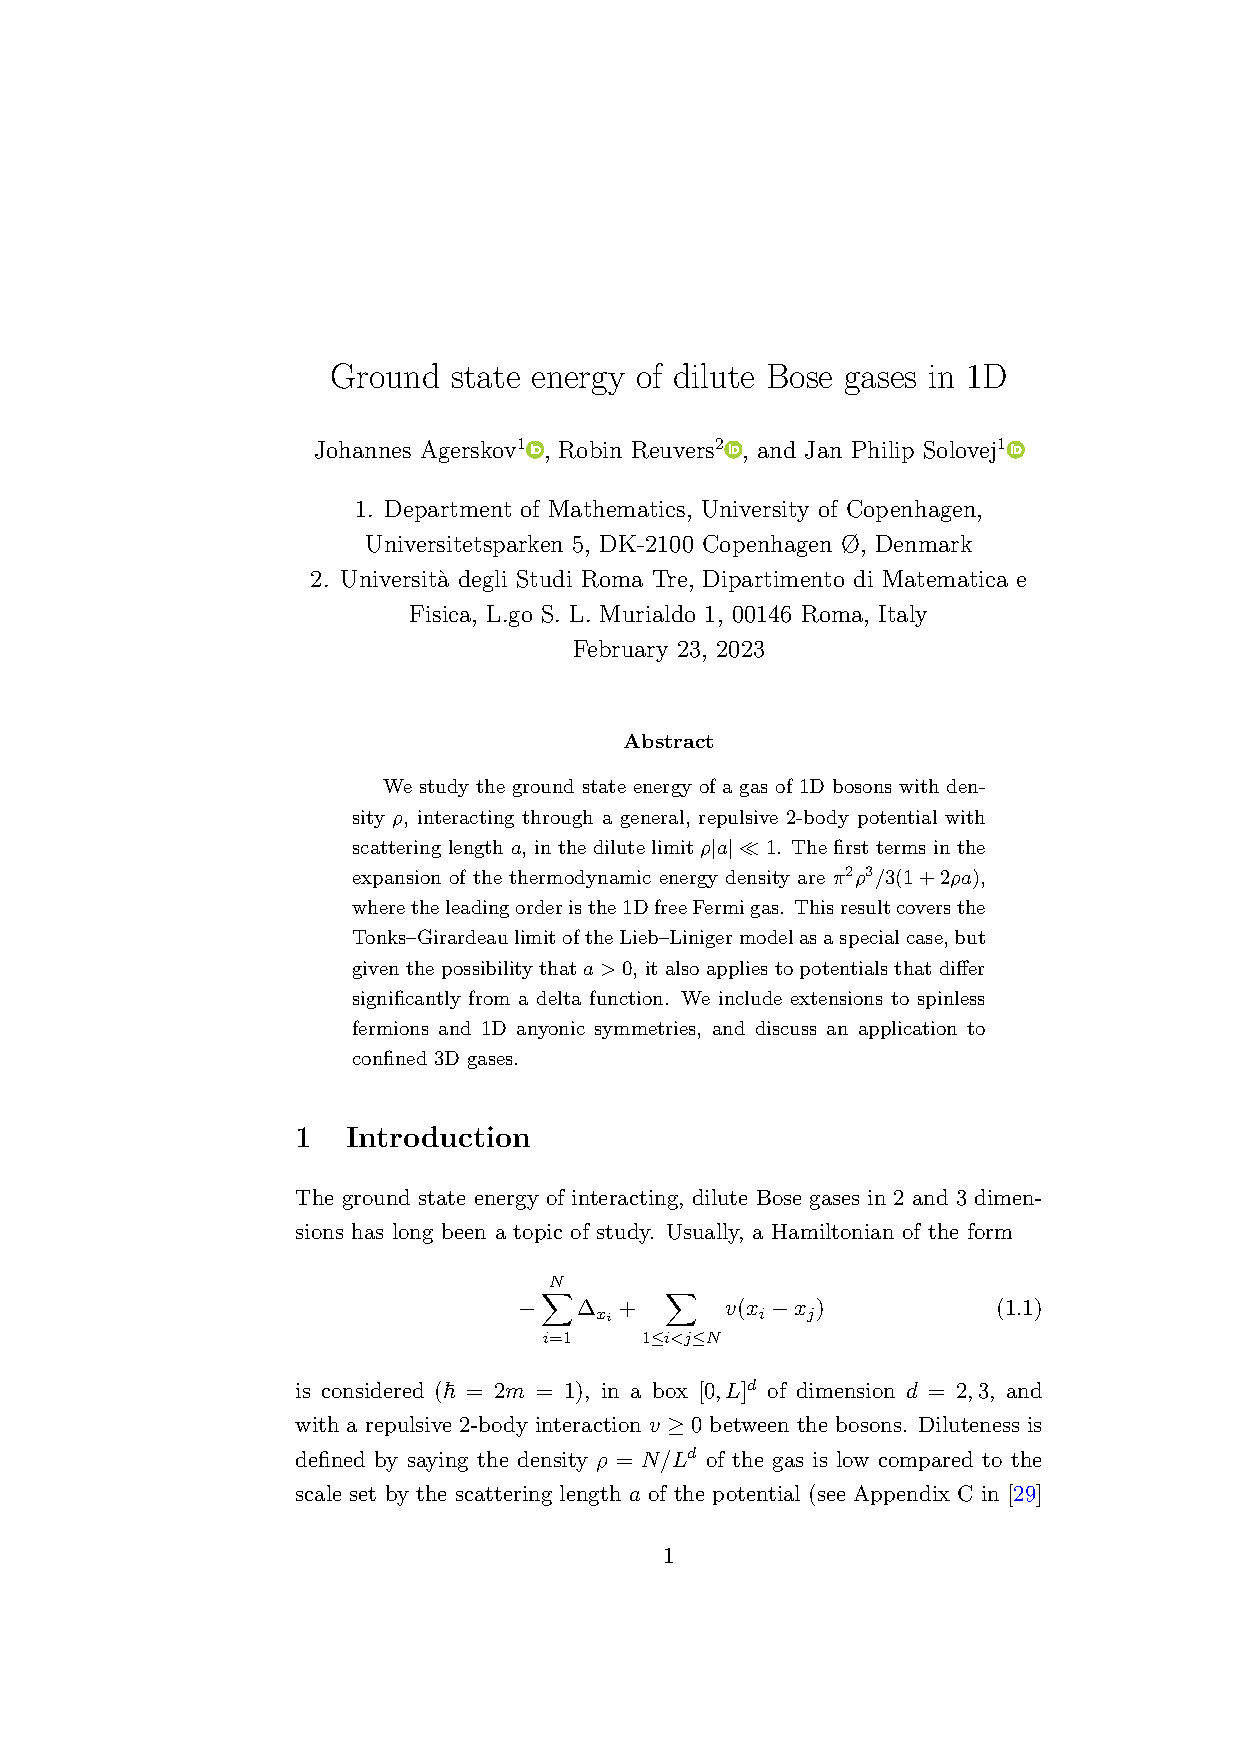
\includepdf[pages={1-},pagecommand={}]{/home/johannes/Documents/Phd/1d bosons draft/one_d_bosons_vThesis.pdf}
\chapter{The Ground State Energy of the One-dimensional Dilute Spin--$ \frac{1}{2} $ Fermi Gas}
\label{ChapterTheGroundStateEnergyOfTheOneDimensionalDiluteSpin1/2FermiGas}
In the preprint of Chapter \ref{ChapterTheGroundStateEnergyOfTheOneDimensionalDiluteBoseGas}, we proved an upper and a lower bound for the ground state energy of a dilute Bose gas in one dimension. It was also shown that, as a corollary, the ground state energy of a one-dimensional dilute spin polarized Fermi gas admitted similar bounds. In this chapter, we seek to analyze instead the full spin--1/2 Fermi gas. Due to an important theorem of Lieb and Mattis, \cite{lieb1962theory}, it is known that the ground state of a repulsively interacting spin--1/2 Fermi gas (with an even number of particles), will have vanishing total spin. Therefore, does our bound essentially give estimates on the total spin $ 0 $ sector of the one-dimensional dilute spin--1/2 Fermi gas.
\section{The Model}
We consider a gas of fermions, each with spin--1/2, interacting through a repulsive pair potential $ v\geq 0 $. The assumptions on $ v $ will be similar to those in Chapter \ref{ChapterTheGroundStateEnergyOfTheOneDimensionalDiluteBoseGas}, \ie $ v $ has compact support, say in the ball $ B_{R_0} $, and can be decomposed in $ v=v_{\text{reg}}+v_{\text{h.c.}} $ , where $ v_{\text{reg}} $ is a finite measure and $ v_{\text{h.c.}} $ is a positive linear combination of hard cores. Formally, we write the Hamiltonian \begin{equation}\label{EqFermi1/2Hamiltonian}
H=-\sum_{i=1}^{N}\partial_i^2+\sum_{1\leq i<j\leq N} v(x_i-x_j),
\end{equation}
and with a domain contained in the Hilbert space $ L^2_{\text{as}}\left(\left([0,L]\times \{0,1\}\right)^N\right)\cong \left(L^2([0,L])\otimes \C^2\right)^{\wedge N} $.
We recap here the conjecture, from Remark 6 of Chapter \ref{ChapterTheGroundStateEnergyOfTheOneDimensionalDiluteBoseGas}, about the ground state energy for such a system. \begin{conjecture}\label{ConjectureEqCSpin1/2FermiGroundStateEnergy}
	Let $ v\geq0 $ satisfy the assumption from above, then the ground state energy of the dilute spin--$ 1/2 $ Fermi gas satisfies\begin{equation}\label{EqConjectureEqCSpin1/2FermiGroundStateEnergy}
	E=N\frac{\pi^2}{3}\rho^2\left(1+2\rho \left(\ln(2) a_e+(1-\ln(2))a_o\right)+\mathcal{O}(\rho^2\max(\abs{a_e},a_o)^2)\right).
	\end{equation}
\end{conjecture}
\section{Upper Bound}
\label{SectionSpin1/2FermiUpperBound}
In this section, we prove an upper bound for the ground state energy of the model \eqref{EqFermi1/2Hamiltonian}. The upper bound match, to next-to-leading order, Conjecture \ref{ConjectureEqCSpin1/2FermiGroundStateEnergy}.
To prove the desired upper bound, some prerequisites are needed. We have already covered the definition of the scattering length and scattering wave function in Chapter \ref{ChapterMany-BodyQuantumMechanics}, and the free Fermi ground state was found in Chapter \ref{ChapterTheGroundStateEnergyOfTheOneDimensionalDiluteBoseGas}. For the spin--$ 1/2 $ gas, we furthermore need knowledge about how to handle the spin degrees of freedom. For this purpose, we give some heuristic arguments based on physical intuition and utilize this intuition in constructing a trial state giving the correct upper bound. 
The main result of this section is the following theorem.
\begin{theorem}\label{TheoremUpperBoundSpin1/2Fermi}
	Let $ v\geq0 $ satisfy the assumption from above, then the ground state energy of the dilute spin--$ 1/2 $ Fermi gas satisfies\begin{equation}\label{EqUpperBoundSpin1/2Fermi}
	E\leq N\frac{\pi^2}{3}\rho^2\left(1+2\rho \left(\ln(2) a_e+(1-\ln(2))a_o\right)+\mathcal{O}\left((\rho R)^{6/5}+N^{-1}\right)\right),
	\end{equation}
	with $ R=\max(\abs{a_e}, a_o, R_0) $.
\end{theorem}
\subsection{Constructing a trial state}
In constructing a trial state for the dilute Fermi gas, we may restrict to a sector of the form $ \{\sigma\}=\{\sigma_1,\sigma_2,\ldots,\sigma_N\}=\{0<x_{\sigma_1}<x_{\sigma_2}<\ldots<x_{\sigma_N}<L\} $, then the trial state is given by anti-symmetrically extending to other sectors. Of course, this means that certain boundary conditions need to be satisfied at the boundary $ \{x_{\sigma_i}=x_{\sigma_{i+1}}\} $ for this extension to be in the relevant domain. This boundary condition is exactly that $ \operatorname{P}_t^{i,i+1} \Psi\rvert_{\{x_{\sigma_i}=x_{\sigma_{i+1}}\}}=0 $. Here $ \operatorname{P}_t^{i,j} $ denotes the spin-projection onto the triplet of particles $ i $ and $ j $, and equivalently we will denote the spin-projection onto the singlet of particles $ i $ and $ j $ by $ \operatorname{P}_s^{i,j} $. We recall from Chapter \ref{ChapterTheGroundStateEnergyOfTheOneDimensionalDiluteBoseGas} that the ground state energy (of the Bose gas or spin polarized Fermi gas) may be well approximated in the dilute limit, by a state that resembles a free Fermi state when particles are far apart, and resembles the two-particle scattering solution when a pair is close. With this in mind, we may construct a variational state trial state on a sector $ \{1,2,\ldots,N\} $ as follows\begin{equation}\label{EqTrial StateSpin1/2Fermi}
\Psi_\chi=\begin{cases}
\frac{\Psi_F}{\mathcal{R}}\left(\left(\eta\omega^{\mathcal{R}}_e+(1-\eta)\omega^{\mathcal{R}}_o\right)\operatorname{P}_s^{\mathcal{R}}+\omega_o^{\mathcal{R}}\operatorname{P}_t^{\mathcal{R}}\right)\chi,&\mathcal{R}(x)<b\\
\Psi_F,&\mathcal{R}(x)\geq b
\end{cases},
\end{equation}
where $ \chi $ is some spin state, $ b>R_0 $, $ \mathcal{R}(x)=\min_{i,j}\abs{x_i-x_j} $, $ \omega^\mathcal{R}_{s/o}(x)\coloneqq \omega_{s/o}(\mathcal{R}(x)) $, and for $\mathcal{R}(x)=\abs{x_i-x_j}$, we have $ \operatorname{P}_{s/t}^{\mathcal{R}(x)}:=\operatorname{P}_{s/t}^{h(i),h(j)} $ with $h(i)$ being the spin-index of the particle with coordinate $x_i$\footnote{\label{FootnoteSpinProjection}When we are on the sector $ \{\sigma\} $ and we are defining $$ \Psi\left((x_{\sigma_1},s_{\sigma_1}),(x_{\sigma_2},s_{\sigma_2}),\ldots,(x_{\sigma_N},s_{\sigma_N})\right), $$ we have $h(i)=i$. On the other hand, if we seek to define $$\Psi\left((x_{\sigma_1},s_1),(x_{\sigma_2},s_2),\ldots,(x_{\sigma_N},s_N)\right),$$ we have $ h(i)=\sigma^{-1}(i) $. This is only relevant for considering symmetries different from the fermionic spin-space anti-symmetry, as $$
	\Psi\left((x_{1},s_{1}),(x_{2},s_{2}),\ldots,(x_{N},s_{N})\right)=\text{sgn}(\sigma)\Psi\left((x_{\sigma_1},s_{\sigma_1}),(x_{\sigma_2},s_{\sigma_2}),\ldots,(x_{\sigma_N},s_{\sigma_N})\right),
	$$
	for fermionic wave functions. Hence, in this section, we may as well think of $ h $ as $h(i)=i$.
	 A different symmetry is considered below in Section \ref{SectionExtendingTheUpperBoundOtherSymmetries}.}. Furthermore, $ \eta $ is a continuous and almost everywhere differentiable function with the property $ \eta(x)=0 $ when $ \mathcal{R}_2(x)=b $, where $ \mathcal{R}_2(x)=\min_{(i,j)\neq (k,l)}\max(\abs{x_i-x_j},\abs{x_k-x_l}) $ is the distance between the second closest pair. More precisely we define
\begin{equation}
\eta(x)\coloneqq\begin{cases}
0,&\text{ if } \mathcal{R}_2(x)\leq b\\
\left(\frac{\mathcal{R}_2(x)}{b}-1\right), &\text{ if } b<\mathcal{R}_2(x)<2b\\
1, &\text{ if } \mathcal{R}_2(x)\geq 2b.
\end{cases}
\end{equation}
In this case, we see that $ \operatorname{P}_t^{i,j}\Psi\rvert_{x_i=x_j}=0 $ due to the boundary condition satisfied by $ \omega_o $. We notice that a potential discontinuity could arise from $ \operatorname{P}_{s/t}^{\mathcal{R}(x)} $, since these projection are discontinuous at points where $ \mathcal{R}_2(x)=\mathcal{R}(x) $. However, since $ \operatorname{P}_{s}^{\mathcal{R}(x)}+\operatorname{P}_{t}^{\mathcal{R}(x)}=1 $, we see that $ \Psi $ is continuous due to the inclusion of $ \eta $. The extension of $ \Psi $ to other sectors $ \{\sigma\} $ is then defined by anti-symmetry in the space-spin variables. In this case, due to the symmetry of the Hamiltonian/energy quadratic form, the energy is determined completely by the energy on the sector $ \{1,2,\ldots,N\} $.\\
As was the case in Chapter \ref{ChapterTheGroundStateEnergyOfTheOneDimensionalDiluteBoseGas}, the trial state given in \eqref{EqTrial StateSpin1/2Fermi} produces an error that grows with the particle number. This is undesirable for proving Theorem \ref{TheoremUpperBoundSpin1/2Fermi}. However, as before, we may construct the full trial state by localizing it to smaller intervals. This is done by splitting the interval $ [0,L] $ into smaller intervals $ I_m\coloneqq[m(\ell+b),(m+1)\ell+mb] $ $ m=0,1,2,\ldots M-1 $, where $ \ell=L/M-b $. We then consider the trial state given by a product \begin{equation}\label{EqFullTrialStateSpin1/2}
\Psi_{\chi,\text{full}}(x_1,\ldots,x_N)=\prod_{m=0}^{M-1}\Psi^{I_m}_{\chi}(x_1^m,\ldots,x_{\tilde{N}}^m),
\end{equation}
where $ \tilde{N}=N/M $ and $ x_i^m\coloneqq x_{m\tilde{N}+i} $ and the superscribt $ I_m $ in $ \Psi^{I_m}_{\chi} $ means that we take the state $ \Psi_{\chi} $ constructed on $ I_m $ instead of $ [0,L] $. Notice that there are no interactions between boxes since $ b>R_0 $. 
\begin{remark}\label{RemarkTechnicalDetailTheoremUpperBoundProof}
	Of course, dividing the particles in this way, might not be possible with desirable integers $\tilde{N}$ and $ M $. However, for a desirable $\tilde{N}$ (not necessarily integer), we may take $M=\ceil{ N/\tilde{N}}$, and then the particles in each box will be $\ceil{N/M}$ or $\ceil{N/M-1}$ in such a way that the total number of particles remain $N$. In this case, the length of a given box may also be chosen, according to the number of particles it contains, to be $\ell_{\ceil{N/M}}=\rho^{-1}\ceil{N/M}-b$ and $ \ell_{\ceil{N/M-1}}=\rho^{-1}\ceil{N/M-1}-b $. This technical detail produces only errors that are small compared to existing errors in the proof of Theorem \ref{TheoremUpperBoundSpin1/2Fermi} below, and thus for simplicity we ignore it.
\end{remark}
 We saw in Chapter \ref{ChapterTheGroundStateEnergyOfTheOneDimensionalDiluteBoseGas} that the scattering solution, when particles are close, leads to a correction to the free Fermi energy that is of order $ 2\rho a_{e/o} E_F $. Since $ \operatorname{P}_s^{i,j}=1/4-S_i\cdot S_j $ and $ \operatorname{P}_t^{i,j}=3/4+S_i\cdot S_j $, we expect (ignoring the effect of $ \eta $) that the correction we obtain from the variational state $ \Psi_\chi $ is of the order $$
2\rho\left( (a_o-a_e) \braket{\chi \left\vert \frac{1}{N}\sum_{i}S_i\cdot S_{i+1} \right\vert \chi} +\frac{1}{4}a_e+\frac{3}{4}a_o \right)E_F.
$$ 
The minimizer (in $ \chi $) $ \chi_0 $ is known, and in this case, since $ a_o\geq a_e $, it is given by the ground state of the periodic antiferromagnetic Heisenberg chain $ \chi_0=\ket{\text{GS}_{\text{HAF}}} $. This ground state is known explicitly, as it is of Bethe ansatz form \cite{bethe1931theorie}. Furthermore, the ground state energy of the antiferromagnetic Heisenberg chain is known to be \cite{hult1938,mattis2012theory} (See lemma \ref{LemmaHeisenbergChainFiniteNEstimate} below) \begin{equation}
\braket{\text{GS}_{\text{HAF}} \left \lvert \frac{1}{N}\sum_{i}S_i\cdot S_{i+1} \right\rvert \text{GS}_{\text{HAF}}}=\frac{1}{4}-\ln(2)+\mathcal{O}(1/N).
\end{equation}
Hence we find the correction $ 2\rho \left(\ln(2)a_e+(1-\ln(2))a_o\right)E_F $ as desired.
\subsection{Proof of Theorem \ref{TheoremUpperBoundSpin1/2Fermi}}
In this section, we give the rigorous proof of Theorem \ref{TheoremUpperBoundSpin1/2Fermi}. The idea was already sketched in the previous section, and the goal is thus to make the statements in the previous section rigorous. An important, although completely trivial, fact is the following lemma. \begin{lemma}\label{LemmaEtaDerivative}
	Let $ \eta $ be defined as above, then we have \begin{equation}
	\abs{\nabla\eta}\leq \frac{\sqrt{2}}{b}, \textnormal{ a.e}.
	\end{equation}
\end{lemma}
The quantity of interest in the following will be the energy of the trial state\begin{equation}
\mathcal{E}(\Psi_\chi)=\int_{[0,L]^N}\sum_{i=1}^{N} \abs{\partial_i\Psi_\chi}^2+\sum_{1\leq i<j\leq N}v_{ij}\abs{\Psi_\chi}^2.
\end{equation}
We will henceforth assume $ \chi $ to be translation invariant. This assumption is not needed, when we have periodic boundary conditions, see Appendix \ref{AppendixPeriodicBCSpin1/2}.
As was done in Chapter \ref{ChapterTheGroundStateEnergyOfTheOneDimensionalDiluteBoseGas}, we rewrite this by use of the diamagnetic inequality\begin{equation}\label{EqEnergy1Spin1/2}
\begin{aligned}
\mathcal{E}(\Psi_\chi)&\leq E_F + \int_{B}\sum_{i=1}^{N}\abs{\partial_i\Psi_{\chi}}^2+\sum_{1\leq i<j\leq N}v_{ij}\abs{\Psi_{\chi}}^2-\sum_{i=1}^{N}\abs{\partial_i \Psi_F}^2\\
&=E_F+\binom{N}{2}\int_{B_{12}}\sum_{i=1}^{N}\abs{\partial_i\Psi_{\chi}}^2+\sum_{1\leq i<j\leq N}v_{ij}\abs{\Psi_{\chi}}^2-\sum_{i=1}^{N}\abs{\partial_i \Psi_F}^2,
\end{aligned}
\end{equation}
where $ B=\{x\in [0,L]^N \vert \mathcal{R}(x)<b\} $, and $ B_{12}=\{x\in [0,L]^N\vert \mathcal{R}(x)=\abs{x_1-x_2}<b\} $. Now due to the presence of $ \eta $ in the trial state, we need to further divide the integration domain. We list here different domains of integration that will be relevant in this section \begin{equation}
\begin{aligned}
B^{\geq}_{12}&=B_{12}\cap \{\mathcal{R}_2(x)\geq 2b\},\\
B^{23}_{12}&=B_{12}\cap\{\mathcal{R}_2(x)=\abs{x_2-x_3}<2b\},\\
B^{34}_{12}&=B_{12}\cap\{\mathcal{R}_2(x)=\abs{x_3-x_4}<2b\},\\
A_{12}&=\left\{x\in [0,L]^N\ \big\vert \abs{x_1-x_2}<b\right\},\\
A_{12}^{23}&=A_{12}\cap \{\abs{x_2-x_3}<2b\},\\
A_{12}^{34}&=A_{12}\cap \{\abs{x_3-x_4}<2b\}.
\end{aligned}
\end{equation} 
In \eqref{EqEnergy1Spin1/2} the last term is dealt with in the same way as in Chapter \ref{ChapterTheGroundStateEnergyOfTheOneDimensionalDiluteBoseGas}. It is also obvious that we may replace $ v $ by $ v_{\text{reg}} $, as the trial state vanishes whenever a pair is inside the outermost hard core. Now due to the anti-symmetry, we conclude from \eqref{EqEnergy1Spin1/2}
\begin{equation}\label{EqEnergy2Spin1/2}
\begin{aligned}
\mathcal{E}(\Psi_{\chi})\leq E_F&+\binom{N}{2}\int_{B_{12}^{\geq}}\sum_{i=1}^{N}\abs{\partial_i\Psi_{\chi}}^2+2(N-2)\binom{N}{2}\int_{B_{12}^{23}}\sum_{i=1}^{N}\abs{\partial_i\Psi_{\chi}}^2\\
&+\binom{N}{2}\binom{N-2}{2}\int_{B_{12}^{34}}\sum_{i=1}^{N}\abs{\partial_i\Psi_{\chi}}^2\\
&+\binom{N}{2}\int_{B_{12}}\sum_{1\leq i<j\leq N}(v_{\text{reg}})_{ij}\abs{\Psi_{\chi}}^2-\binom{N}{2}\int_{B_{12}}\sum_{i=1}^{N}\abs{\partial_i \Psi_F}^2.
\end{aligned}
\end{equation}
%Now we define 
%\begin{equation}\label{EqTrialState12}
%(\tilde{\Psi}_\chi)_{12}\coloneqq \Psi_{\chi}\big\rvert_{B_{12}^\geq},
%\end{equation}
%\begin{equation}\label{EqTrialState12}
%(\tilde{\Psi}_\chi)_{12}\coloneqq \frac{\Psi_F}{x_2-x_1}\left(\omega^{12}_e \operatorname{P}_s^{1,2}+\omega_o^{12}\operatorname{P}_t^{1,2}\right)\chi,
%\end{equation}
%and extend $ (\tilde{\Psi}_\chi)_{12} $ to all of $ A_{12} $ by anti-symmetry. By definition we have $ \Psi_{\chi}=(\tilde{\Psi}_\chi)_{12} $ on $ B_{12}^{\geq}\subset A_{12} $, and on $ \{1,2,\ldots,N\}\cap A_{12} $ we have 
%\begin{equation}
%(\tilde{\Psi}_\chi)_{12}\coloneqq \frac{\Psi_F}{x_2-x_1}\left(\omega^{12}_e \operatorname{P}_s^{1,2}+\omega_o^{12}\operatorname{P}_t^{1,2}\right)\chi,
%\end{equation}
Defining \begin{equation}
\begin{aligned}
(\Psi_e)_{12}\coloneqq\frac{\Psi_F}{\abs{x_2-x_1}}\omega_e^{12}\text{ and } (\Psi_o)_{12}\coloneqq\frac{\Psi_F}{\abs{x_2-x_1}}\omega_o^{12},
\end{aligned}
\end{equation}
we find by the fact that $ B_{12}^\geq\subset A_{12} $, \begin{equation}\label{EqEnergy3Spin1/2}
\begin{aligned}
\int_{B_{12}^{\geq}}\abs{\partial_i\Psi_{\chi}}^2\leq&\sum_{\{\sigma\}\in S_{12}}\left(\int_{A_{12}\cap\{\sigma\}}\abs{\partial_i(\Psi_e)_{12}}^2\right)\braket{\chi_{\sigma} \left\lvert \operatorname{P}^{1,2}_s  \right\rvert \chi_\sigma}\\
&+\sum_{\{\sigma\}\in S_{12}}\left(\int_{A_{12}\cap \{\sigma\}}\abs{\partial_i(\Psi_o)_{12}}^2\right)\braket{\chi_{\sigma} \left\lvert \operatorname{P}^{1,2}_t  \right\rvert \chi_\sigma},
\end{aligned}
\end{equation}
where $ \operatorname{P}_{s/t}^{N,N+1}\coloneqq \operatorname{P}_{s/t}^{N,1} $ and $ \chi_{\sigma} $ is the spin state $ \chi $ with spins permuted by $ (1,\ldots,N)\mapsto(\sigma_1,\ldots,\sigma_N) $ and 
$$ S_{12}=\{\text{sectors } \{\sigma\}\ \vert\ (\sigma_k,\sigma_{k+1})=(1,2)\text{ or }(\sigma_k,\sigma_{k+1})=(2,1)\text{ for some }k\}. $$
Using the translation invariance of $ \chi $ we see that 
$$ \braket{\chi_{\sigma} \left\lvert \operatorname{P}^{1,2}_{s/t}  \right\rvert \chi_\sigma}=\frac{1}{N}\sum_{k=1}^{N}\braket{\chi_\sigma\left\lvert \operatorname{P}^{\sigma_k,\sigma_{k+1}}_{s/t}  \right\rvert \chi_\sigma}=\frac{1}{N}\sum_{k=1}^{N}\braket{\chi\left\lvert \operatorname{P}^{k,k+1}_{s/t}  \right\rvert \chi} $$
is independent of $ \sigma\in S_{12} $ and that
\begin{equation}\label{EqEnergy4Spin1/2}
\begin{aligned}
\int_{B_{12}^{\geq}}\abs{\partial_i\Psi_{\chi}}^2\leq&\left(\int_{A_{12}}\abs{\partial_i(\Psi_e)_{12}}^2\right)\frac{1}{N}\sum_{k=1}^{N}\braket{\chi \left\lvert \operatorname{P}^{k,k+1}_s  \right\rvert \chi}\\
&+\left(\int_{A_{12}}\abs{\partial_i(\Psi_o)_{12}}^2\right)\frac{1}{N}\sum_{k=1}^{N}\braket{\chi\left\lvert \operatorname{P}^{k,k+1}_t  \right\rvert \chi},
\end{aligned}
\end{equation}


Considering \eqref{EqEnergy2Spin1/2} again, we see from the trivial relation $$
\frac{1}{N}\left(\sum_{k=1}^{N} \braket{\chi \left\lvert \operatorname{P}^{k,k+1}_s  \right\rvert \chi}+\sum_{k=1}^{N}\braket{\chi \left\lvert \operatorname{P}^{k,k+1}_t  \right\rvert \chi}\right)=1,
$$
and from the fact that $ B_{12}\subset A_{12} $ and the observation that 
$$ \abs{\Psi_{\chi}}^2\leq \frac{1}{N}\sum_{k=1}^{N}\left(\braket{\chi \left\vert P_{s}^{k,k+1} \right\vert\chi}\abs{(\Psi_e)_{12}}^2+\braket{\chi \left\vert P_{t}^{k,k+1} \right\vert\chi}\abs{(\Psi_o)_{12}}^2\right)$$
 on $ B_{12} $ that we have the following upper bound for the energy\begin{equation}\label{EqTrialStateEnergyUpperBound1}
	\begin{aligned}
	\mathcal{E}(\Psi_{\chi})\leq E_F&+\binom{N}{2}\frac{1}{N}\sum_{k=1}^{N}\braket{\chi \left\lvert \operatorname{P}^{k,k+1}_s  \right\rvert \chi}\Bigg(\int_{A_{12}}\sum_{i=1}^{N}\abs{\partial_i(\Psi_e)_{12}}^2\\
	&+\int_{A_{12}}\sum_{1\leq i<j\leq N}(v_{\text{reg}})_{ij}\abs{(\Psi_e)_{12}}^2-\int_{B_{12}}\sum_{i=1}^{N}\abs{\partial_i \Psi_F}^2\Bigg)\\
	&+\binom{N}{2}\frac{1}{N}\sum_{k=1}^{N}\braket{\chi \left\lvert \operatorname{P}^{k,k+1}_t  \right\rvert \chi}\Bigg(\int_{A_{12}}\sum_{i=1}^{N}\abs{\partial_i(\Psi_o)_{12}}^2\\
	&+\int_{A_{12}}\sum_{1\leq i<j\leq N}(v_{\text{reg}})_{ij}\abs{(\Psi_o)_{12}}^2-\int_{B_{12}}\sum_{i=1}^{N}\abs{\partial_i \Psi_F}^2\Bigg)\\
	&+\binom{N}{2}\binom{N-2}{2}\int_{B_{12}^{34}}\sum_{i=1}^{N}\abs{\partial_i\Psi_{\chi}}^2\\
	&+2(N-2)\binom{N}{2}\int_{B_{12}^{23}}\sum_{i=1}^{N}\abs{\partial_i\Psi_{\chi}}^2.
	\end{aligned}
\end{equation}
We see that this reduces proving an upper bound to a case we have already analyzed in Chapter \ref{ChapterTheGroundStateEnergyOfTheOneDimensionalDiluteBoseGas}, except for the last two terms, which we then need to estimate. Let us denote the two quantities by \begin{equation}
\begin{aligned}
E_{12}^{34}&\coloneqq\binom{N}{2}\binom{N-2}{2}\int_{B_{12}^{34}}\sum_{i=1}^{N}\abs{\partial_i\Psi_{\chi}}^2,\\
E_{12}^{23}&\coloneqq 2(N-2)\binom{N}{2}\int_{B_{12}^{23}}\sum_{i=1}^{N}\abs{\partial_i\Psi_{\chi}}^2.
\end{aligned}
\end{equation} 
The following lemmas, which we prove below, provide estimates of these quantities.
\begin{lemma}\label{LemmaSpin1/2EtaContribution1}
	Let $ E_{12}^{34} $ and $ \Psi_{\chi} $ be defined as above, then we have the following bound:\begin{equation}
	E_{12}^{34}\leq \textnormal{ const. } E_F\left(N\left(\rho b\right)^4+N^2\left(\rho b\right)^6 \right).
	\end{equation}
	where $ E_F $ denotes the free spin polarized (spinless) Fermi energy.
\end{lemma}

\begin{lemma}\label{LemmaSpin1/2EtaContribution2}
	Let $ E_{12}^{23} $ and $ \Psi_{\chi} $ be defined as above, then we have the following bound:\begin{equation}
	E_{12}^{23}\leq \textnormal{ const. } E_F\left(\left(\rho b\right)^4+N\left(\rho b\right)^6 \right).
	\end{equation}
	where $ E_F $ denotes the free spin polarized (spinless) Fermi energy.
\end{lemma}
Using Lemmas \ref{LemmaSpin1/2EtaContribution1} and \ref{LemmaSpin1/2EtaContribution2}, we deduce, from \eqref{EqTrialStateEnergyUpperBound1} the following bound upper bound on the trial state energy
\begin{equation}\label{EqSpin1/2EnergyUpperBound}
\begin{aligned}
\mathcal{E}(\Psi_{\chi})\leq E_F&+\binom{N}{2}\frac{1}{N}\sum_{k=1}^{N}\braket{\chi \left\lvert \operatorname{P}^{k,k+1}_s  \right\rvert \chi}\Bigg(\int_{A_{12}}\sum_{i=1}^{N}\abs{\partial_i(\Psi_e)_{12}}^2\\
&+\int_{A_{12}}\sum_{1\leq i<j\leq N}(v_{\text{reg}})_{ij}\abs{(\Psi_e)_{12}}^2-\int_{B_{12}}\sum_{i=1}^{N}\abs{\partial_i \Psi_F}^2\Bigg)\\
&+\binom{N}{2}\frac{1}{N}\sum_{k=1}^{N}\braket{\chi \left\lvert \operatorname{P}^{k,k+1}_t  \right\rvert \chi}\Bigg(\int_{A_{12}}\sum_{i=1}^{N}\abs{\partial_i(\Psi_o)_{12}}^2\\
&+\int_{A_{12}}\sum_{1\leq i<j\leq N}(v_{\text{reg}})_{ij}\abs{(\Psi_o)_{12}}^2-\int_{B_{12}}\sum_{i=1}^{N}\abs{\partial_i \Psi_F}^2\Bigg)\\
&+E_F\left(N(\rho b)^4+ N^2 (\rho b)^6\right).
\end{aligned}
\end{equation}
Defining the quantities \begin{equation}
\begin{aligned}
E_{1,e}\coloneqq\binom{N}{2}\Bigg(\int_{A_{12}}\sum_{i=1}^{N}\abs{\partial_i(\Psi_e)_{12}}^2
&+\sum_{1\leq i<j\leq N}(v_{\text{reg}})_{ij}\abs{(\Psi_e)_{12}}^2-\sum_{i=1}^{N}\abs{\partial_i \Psi_F}^2\Bigg),\\
E_{1,o}\coloneqq\binom{N}{2}\Bigg(\int_{A_{12}}\sum_{i=1}^{N}\abs{\partial_i(\Psi_o)_{12}}^2
&+\sum_{1\leq i<j\leq N}(v_{\text{reg}})_{ij}\abs{(\Psi_o)_{12}}^2-\sum_{i=1}^{N}\abs{\partial_i \Psi_F}^2\Bigg),
\end{aligned}
\end{equation}
and the quantities from Chapter \ref{ChapterTheGroundStateEnergyOfTheOneDimensionalDiluteBoseGas}:\begin{equation}
\begin{aligned}
E_2^{(1)}&\coloneqq\binom{N}{2}2N\int_{A_{12}\cap A_{13}}\sum_{i=1}^{N}\abs{\partial_i\Psi_F}^2,\\ E_2^{(2)}&\coloneqq\binom{N}{2}\binom{N-2}{2}\int_{A_{12}\cap A_{34}}\sum_{i=1}^{N}\abs{\partial_i\Psi_F}^2,
\end{aligned}
\end{equation}
we see by noting $x\in A_{12}\setminus B_{12}$ implies $x\in A_{12}\cap A_{ij}$ for some $\{i,j\}\neq \{1,2\}$ that \eqref{EqSpin1/2EnergyUpperBound} implies \begin{equation}\label{EqTrialStateEnergyUpperBound2}
\begin{aligned}
\mathcal{E}(\Psi_{\chi})\leq E_F &+\frac{1}{N}\sum_{k=1}^{N}\braket{\chi \left\lvert \operatorname{P}^{k,k+1}_s  \right\rvert \chi} \left(E_{1,e}+E_2^{(1)}+E_2^{(2)}\right)\\
&+\frac{1}{N}\sum_{k=1}^{N}\braket{\chi \left\lvert \operatorname{P}^{k,k+1}_t  \right\rvert \chi} \left(E_{1,o}+E_2^{(1)}+E_2^{(2)}\right)\\
&+E_F\left(N(\rho b)^4+ N^2 (\rho b)^6\right)
\end{aligned}
\end{equation}
Here $ E_{1,e/o} $ corresponds to the quantity $ E_1 $ in Chapter \ref{ChapterTheGroundStateEnergyOfTheOneDimensionalDiluteBoseGas} with the even/odd wave scattering solution in the trial state. Proving the equivalent bound for the $ E_{1,e/o} $ amounts to following the same proof strategy and we have the equivalent lemma:
\begin{lemma}[Lemma 13 of Chapter \ref{ChapterTheGroundStateEnergyOfTheOneDimensionalDiluteBoseGas}]\label{LemmaE1BoundSpin1/2}
	Let $ E_{1,e/o} $ be defined as above. For $ b>\max(2a_o,R_0) $ we have \begin{equation}
	\begin{aligned}
	E_{1,e/o}\leq E_F&\Bigg(2\rho a_{e/o}\frac{b}{b-a_{e/o}}\\&+ \textnormal{const. }\left( N(\rho b)^3\left[ 1+ \rho b^2\int v_{\textnormal{reg}}\right]+\rho a_{e/o} \frac{\ln(N)}{N}\right)\Bigg).
	\end{aligned}
	\end{equation}
\end{lemma}
We also recall the lemma\begin{lemma}[Lemma 14 of Chapter \ref{ChapterTheGroundStateEnergyOfTheOneDimensionalDiluteBoseGas}]\label{LemmaE2BoundSpin1/2}
	\begin{equation}
	E_2^{(1)}+E_2^{(2)}\leq E_F\left(N (\rho b)^4+ N^2(\rho b)^6\right).
	\end{equation}
\end{lemma}
Using Lemmas \ref{LemmaE1BoundSpin1/2} and $ \ref{LemmaE2BoundSpin1/2} $ we find the result 
\begin{lemma}\label{LemmaTrialStateEnergySpin1/2}
	For $ N(\rho b)^3\leq  1 $ and $ b>\max(2 a_o,R_0) $ we have \begin{equation}\label{EqTrialStateEnergyBound1}
	\begin{aligned}
	\mathcal{E}(\Psi_{\chi})\leq E_F\Bigg( 1&+2\rho\left[\frac{1}{4}\tilde{a}_e+\frac{3}{4}\tilde{a}_o+(\tilde{a}_o-\tilde{a}_e)\frac{1}{N}\braket{\chi \left\vert \sum_{k=1}^N S_k\cdot S_{k+1}\right\vert \chi}\right]\\ &+\textnormal{ const. }\left( N (\rho b)^3\left[1+\rho b^2\int v_{\textnormal{reg}}\right]+\rho a_o \frac{\ln(N)}{N}\right) \Bigg),
	\end{aligned}
	\end{equation}
	where $ \tilde{a}_{e/o}\coloneqq a_{e/o}\frac{b}{b-a_{e/o}} $.
\end{lemma}
\begin{proof}
	This lemma follows directly by combining \eqref{EqTrialStateEnergyUpperBound2} with Lemmas \ref{LemmaE1BoundSpin1/2} and \ref{LemmaE2BoundSpin1/2}.
\end{proof}
It is then immediately clear that on the right-hand side of \eqref{EqTrialStateEnergyBound1}, given that $ a_o>a_e $, the optimal choice for $ \chi $ is the ground state of the periodic antiferromagnetic Heisenberg chain, which due to the Marshall-Lieb-Mattis theorem, \cite{lieb1962ordering,marshall1955antiferromagnetism}, is translation invariant. Of course, if $ a_o=a_e $, the choice of $ \chi $ is irrelevant for the right-hand side of \eqref{EqTrialStateEnergyBound1}. \\
We thus conclude that the ground state energy of the antiferromagnetic Heisenberg chain is of importance. Fortunately, this model is exactly solvable, as shown by Bethe \cite{bethe1931theorie}, and the ground state energy can be found in the thermodynamic limit, as shown by Hulthén \cite{hult1938}: \begin{lemma}[\cite{mattis2012theory}, Eq. (5.171)]\label{LemmaHeisenbergChainThermodynamicGSEnergy}
Let $ \ket{\textnormal{GS}_{\textnormal{HAF}}} $ denote the ground state of the periodic antiferromagnetic Heisenberg chain. Then\begin{equation}
\lim\limits_{N\to\infty}\braket{\textnormal{GS}_{\textnormal{HAF}}\Bigg\vert\frac{1}{N}\sum_{k=1}^N S_k\cdot S_{k+1} \Bigg\vert \textnormal{GS}_{\textnormal{HAF}}}=\frac{1}{4}-\ln(2) 
\end{equation}
\end{lemma}
This lemma gives the ground state energy of the Heisenberg chain in the thermodynamic limit, however, we need an estimate for the finite chain. This is given by the following lemma:
\begin{lemma}\label{LemmaHeisenbergChainFiniteNEstimate}
	Let $ \ket{\textnormal{GS}_{\textnormal{HAF}}} $ denote the ground state of the periodic antiferromagnetic Heisenberg chain. Then\begin{equation}
	\braket{\textnormal{GS}_{\textnormal{HAF}}\Bigg\vert\frac{1}{N}\sum_{k=1}^N S_k\cdot S_{k+1} \Bigg\vert \textnormal{GS}_{\textnormal{HAF}}}=\frac{1}{4}-\ln(2) +\mathcal{O}(N^{-1})
	\end{equation}
\end{lemma}
\begin{proof}
	Denoting the Dirichlet (edge spin down) energy of the spin chain $ E_D^N $ with $ N $ sites and the periodic energy $ E_P^N $, we have $ E_P^N\leq E_D^N $. 
	This follows directly from the variational principle.
%	To see this notice that the Dirichlet ground state is given as the ground state of the Hamiltonian $ H_D=\sum_{k=1}^{N} S_{k}\cdot S_{k+1}+ B_e(1+S_1^z+S_N^z) $ for large enough $ B_e>0 $. Since $ H_D\geq H_{\text{HAF}} $ and since $ B_e(1+S_1^z+S_N^z) $ vanishes in the Dirichlet ground state, we see that \begin{equation}
%	E_D^N=\braket{\sum_{k=1}^{N} S_{k}\cdot S_{k+1}}_D\geq \braket{\sum_{k=1}^{N} S_{k}\cdot S_{k+1}}_P=E_P^N ,
%	\end{equation}
%	where the subscripts refer to Dirichlet and periodic ground state expectations.
On the other hand we have the following bound \begin{equation}\label{EqDirichletPeriodicSpinChainBound}
E_D^{N+2}\leq E_P^N+\frac{3}{4}.
\end{equation}
To see this, consider a periodic chain of length $ N $ in its ground state. Add a spin-down at each edge, making the chain of length $ N+2 $. The resulting state is now a trial state for the Dirichlet chain of energy at most $ E_P^N+\frac{3}{4} $ and \eqref{EqDirichletPeriodicSpinChainBound} follows. Furthermore, it is not hard to see that for any integer $ m\geq 1 $ we have $ E_D^{mN}\leq E_D^{mN-m+1}\leq mE_D^N $. The first inequality follows simply from the fact that extending a Dirichlet state by Néel ordering (alternating spin) to a larger chain, lowers the energy, hence ground state energy in the larger chain must also be lower. The second inequality follows by constructing a trial state for the Dirichlet chain of length $ mN-m+1 $ by gluing $ m $ ground states of the Dirichlet chain of length $ N $, such that they share a spin down at the gluing points. Collecting everything we have \begin{equation}
\frac{1}{mN}E_P^{mN}\leq \frac{1}{mN}E_D^{mN}\leq \frac{1}{N}E_D^N\leq \frac{1}{N}\left(E_P^{N-2}+3/4\right).
\end{equation}
It is clear that by a trial state argument and by translation invariance, which follows from the Marshall-Lieb-Mattis theorem (uniqueness of the ground state), we have $ E_P^N\leq \frac{N}{M+1}E_P^M+\frac{1}{4} $ for $ M>N $, simply take the ground state of chain length $ M $ and truncate it at length $ N $. Hence we get \begin{equation}
\frac{1}{mN}E_P^{mN}\leq\frac{N-2}{N}\frac{1}{N-2}\left(E_P^{N-2}+3/4\right)\leq \frac{N-2}{N} \left(\frac{1}{M}E^{M}_P +\frac{3}{2}\frac{1}{N-2}\right)
\end{equation}
taking the limits $ m\to \infty $ and $ M\to\infty $ we have \begin{equation}
\frac{N}{N-2}e_P-\frac{3}{4N}\leq\frac{1}{N-2}E_P^{N-2}\leq e_P+\frac{1}{4}\frac{1}{N-2},
\end{equation}
where $ e_P=\lim\limits_{N\to\infty}\frac{1}{N}E_P^N $. The desired result follows from Lemma \ref{LemmaHeisenbergChainThermodynamicGSEnergy}.
\end{proof}
We are now ready to collect everything to give the proof of Theorem \ref{TheoremUpperBoundSpin1/2Fermi}:
\begin{proof}[Proof of Theorem \ref{TheoremUpperBoundSpin1/2Fermi}]
	Consider now the full trial state as given in \eqref{EqFullTrialStateSpin1/2} (See optionally Remark \ref{RemarkTechnicalDetailTheoremUpperBoundProof}). Because of the spacing between intervals, $ I_m $, there are no interactions between particles in different intervals. Hence the energy of such a state \begin{equation}
	\mathcal{E}(\Psi_{\chi,\text{full}})/\norm{\Psi_{\chi,\text{full}}}=M\mathcal{E}(\Psi_{\chi}^{I_0})/\norm{\Psi^{I_0}_{\chi}}.
	\end{equation}
	Combining lemmas \ref{LemmaTrialStateEnergySpin1/2} and \ref{LemmaHeisenbergChainFiniteNEstimate}, we find \begin{equation}
	\begin{aligned}
	\mathcal{E}(\Psi_{\chi,\text{full}})\leq N\frac{\pi^2}{3}\tilde{\rho}^2\Bigg(1&+2\tilde{\rho}\left[\ln(2)\tilde{a}_e+(1-\ln(2))\tilde{a}_o\right]+\text{const. }\frac{M}{N}\\&+\text{ const. }\left(\frac{N}{M}(\tilde{\rho} b)^3 \left[1+\tilde{\rho} b^2\int v_{\text{reg}}\right]+\tilde{\rho} a_o\frac{\ln(N/M)}{N/M}\right)\Bigg),
	\end{aligned}
	\end{equation}
	with $ \rho\leq \tilde{\rho}=\frac{N}{L-Mb}\leq\rho\left(1+2\frac{M}{N}\rho b\right) $ for $ \frac{M}{N}\rho b\leq 1/2 $.\\
	Similarly to the case in Chapter \ref{ChapterTheGroundStateEnergyOfTheOneDimensionalDiluteBoseGas}, term $\tilde{\rho} a_o\frac{\ln(N/M)}{N/M}$ satisfies 
	$$ \tilde{\rho} a_o\frac{\ln(N/M)}{N/M}\leq \max(\text{const. }M/N,C_\epsilon (\tilde{\rho}a_o)^{2-\epsilon}). $$ It is therefore sub-leading and can be absorbed in other error terms. Thus we will neglect this term.\\
	\textbf{For $ N>(\rho b)^{-3/2}\left(1+\rho b^2\int v_{\text{reg}}\right)^{-1/2} $}:\\
	 Choosing $ M/N=(\rho b)^{3/2}\left(1+\rho b^2\int v_{\text{reg}}\right)^{1/2} $ we find \begin{equation}\label{EqSpin1/2TrialStateEnergyBoundFull}
	\begin{aligned}
	\mathcal{E}(\Psi_{\chi,\text{full}})\leq N\frac{\pi^2}{3}&\rho^2\Bigg(1+2\rho\left[\ln(2)\tilde{a}_e+(1-\ln(2))\tilde{a}_o\right]+\\&+\text{ const. }(\rho b)^{3/2} \left(1+\rho b^2\int v_{\text{reg}}\right)^{1/2}\Bigg),
	\end{aligned}
	\end{equation}
	\textbf{For $ N<(\rho b)^{-3/2}\left(1+\rho b^2\int v_{\text{reg}}\right)^{-1/2} $}:\\
	We see that \eqref{EqSpin1/2TrialStateEnergyBoundFull} follows from choosing $ M=1 $.\\
	Furthermore choosing $ b=\max(\rho^{-1/5}\abs{a_e}^{4/5},\rho^{-1/5}a_o^{4/5},R_0) $ we see that $ a_{e/o}\leq \tilde{a}_{e/o}=a_{e/o}\frac{b}{b-a_{e/o}}\leq a_{e/o}\left(1+2(\rho R)^{1/5}\right) $ for $ (\rho R)^{1/5}\leq 1/2 $ and the desired result follows from the simple estimate on the norm\begin{equation}
	\begin{aligned}
	\norm{\Psi^{I_0}_{\chi}}&\geq 1-\int_{A_{12}} \rho^{(2))}(x_1,x_2)\geq 1-\text{ const. }\tilde{N}(\tilde{\rho}b)^3\\&\geq 1-\text{ const. }(\rho b)^{3/2}\geq 1-\text{ const. }(\rho R)^{6/5}.
	\end{aligned}
	\end{equation}
\end{proof}



\subsubsection{Estimating $ E_{12}^{34} $ (proof of lemma \ref{LemmaSpin1/2EtaContribution1})}
\begin{proof}[Proof of Lemma \ref{LemmaSpin1/2EtaContribution1}]
%Estimating $ E_{12}^{34} $ is a straightforward computation that goes as follows:\\ 
%Defining $ \xi_{12}^{34}\coloneqq \left(\left(\eta\omega^{12}_e+(1-\eta)\omega^{12}_o\right)\operatorname{P}_s^{1,2}+\omega_o^{12}\operatorname{P}_t^{1,2}\right)\chi_\sigma $ on $ B_{12}^{34}\cap \{\sigma\} $ for all sectors $ \{\sigma\}\in S_{12}^{34} $, with \begin{equation}
%\begin{aligned}
%S_{12}^{34}\coloneqq\big\{\text{sectors } \{\sigma\}\ \vert \ (1,2)=(\sigma_k,\sigma_{k+1}) \text{ or }\\ (2,1)=(\sigma_k,\sigma_{k+1})\text{ for some } k\\
%\text{ and } (3,4)=(\sigma_l,\sigma_{l+1}) \text{ or }\\ (4,3)=(\sigma_l,\sigma_{l+1})\text{ for some } l\big\}.
%\end{aligned}
%\end{equation}
% We then see that $\Psi_{\chi}=\xi_{12}^{34} \frac{\Psi_F}{\abs{x_2-x_1}}$ on $ B_{12}^{34} $: Hence we find 
%\begin{equation}
%\begin{aligned}
%E_{12}^{34}=&\binom{N}{2}\binom{N-2}{2}\int_{B_{12}^{34}}\sum_{i=1}^{N}\abs{\partial_i\left(\xi_{12}^{34} \frac{\Psi_F}{\abs{x_2-x_1}}\right)}^2\\
%\leq& \binom{N}{2}\binom{N-2}{2}\Bigg[\int_{A_{12}^{34}}\sum_{i=1}^{4}\abs{\partial_i\left(\xi_{12}^{34} \frac{\Psi_F}{\abs{x_2-x_1}}\right)}^2 \\&\qquad+\int_{A_{12}^{34}}\sum_{i=5}^{N}\overline{\xi_{12}^{34} \frac{\Psi_F}{\abs{x_2-x_1}}}\left(\xi_{12}^{34} \frac{(-\partial_i^2\Psi_F)}{\abs{x_2-x_1}}\right)\Bigg]\\
%=& \binom{N}{2}\binom{N-2}{2}\Bigg[\int_{A_{12}^{34}}\sum_{i=1}^{4}\abs{\partial_i\left(\xi_{12}^{34} \frac{\Psi_F}{\abs{x_2-x_1}}\right)}^2 \\&\qquad-\int_{A_{12}^{34}}\sum_{i=1}^{4}\overline{\xi_{12}^{34} \frac{\Psi_F}{\abs{x_2-x_1}}}\left(\xi_{12}^{34} \frac{(-\partial_i^2\Psi_F)}{\abs{x_2-x_1}}\right)\\
%&\qquad + E_F\int_{A_{12}^{34}} \abs{\xi_{12}^{34} \frac{\Psi_F}{\abs{x_2-x_1}}}\Bigg],
%\end{aligned}
%\end{equation}
%where we used $ B_{12}^{34}\subset A_{12}^{34} $, integration by parts, and the fact that $ \Psi_F $ is an eigenfunction of $ (-\Delta) $, with eigenvalue $ E_F $.\\ Thus, using $ \abs{\xi_{12}^{34}}^2\leq b^2 $ and restricting to $ b\geq 2a_0\geq 2a_e $, we find \begin{equation}
%\begin{aligned}
%E_{12}^{34}\leq& 4\! \int_{A_{12}^{34}}\Bigg(\! \sum_{i=1}^{4}\partial_{y_i}\partial_{x_i}\overline{\frac{\xi_{12}^{34}(y)}{\abs{y_2-y_1}}}\frac{\xi_{12}^{34}(x)}{\abs{x_2-x_1}}\gamma^{(4)}(y_1,y_2,y_3,y_4;x_1,x_2,x_3,x_4)\Bigg\rvert_{y=x}\\
%&\qquad\quad+\abs{\frac{\xi_{12}^{34}(x)}{\abs{x_2-x_1}}}^2\abs{\sum_{i=1}^{4}  \partial_{y_i}^2\gamma^{(4)}(y_1,y_2,y_3,y_4;x_1,x_2,x_3,x_4)\Bigg\rvert_{y=x}}\\
%&\qquad\quad+E_F\abs{\frac{\xi_{12}^{34}(x)}{\abs{x_2-x_1}}}^2\rho^{(4)}(x_1,x_2,x_3,x_4)\Bigg)\\
%\leq& \text{ const. } E_F\left(N\left(\rho b\right)^4+N^2\left(\rho b\right)^6 \right)
%\end{aligned}
%\end{equation}
%where we used the following bounds \begin{equation}
%\begin{aligned}
%\partial_{y_i}\partial_{x_i}\frac{\gamma^{(4)}(y_1,y_2,y_3,y_4;x_1,x_2,x_3,x_4)}{\abs{x_2-x_1}\abs{y_2-y_1}}\Bigg \lvert_{y=x}&\leq \text{const.} \rho^{8},\\
%\partial_{y_i}\frac{\gamma^{(4)}(y_1,y_2,y_3,y_4;x_1,x_2,x_3,x_4)}{\abs{x_2-x_1}\abs{y_2-y_1}}\Bigg \lvert_{y=x}&\leq \text{const.} \rho^{8}\abs{x_3-x_4},\\
%\frac{\gamma^{(4)}(y_1,y_2,y_3,y_4;x_1,x_2,x_3,x_4)}{\abs{x_2-x_1}\abs{y_2-y_1}}\Bigg \lvert_{y=x}&\leq \text{const.} \rho^{8}\abs{x_3-x_4}^2,\\
%\abs{\sum_{i=1}^{4}\partial_{y_i}^2\gamma^{(4)}(y_1,y_2,y_3,y_4;x_1,x_2,x_3,x_4) \Bigg \lvert_{y=x}}&\leq \text{const.} \rho^{10} \abs{x_1-x_2}^2\abs{x_3-x_4}^2,
%\end{aligned}
%\end{equation}
%and \begin{equation}
%\rho^{(4)}(x_1,x_2,x_3,x_4)\leq\text{const.} \rho^8 \abs{x_1-x_2}^2\abs{x_3-x_4}^2,
%\end{equation}
%which all follows from Taylor expansion of the free Fermi reduced density (matrices). Furthermore, we used the bounds \begin{equation}
%\sqrt{\abs{\partial_i\xi_{12}^{34}}^2}\leq b \max\left(\frac{\sqrt{2}}{b},\frac{1}{b-a_o}\right)\leq 2,\qquad \sqrt{\abs{\xi_{12}^{34}}^2}\leq b
%\end{equation}
%which follows from properties of the scattering solution, monotonicity of its derivative, and Lemma \ref{LemmaEtaDerivative}.


Estimating $ E_{12}^{34} $ is a straightforward computation that goes as follows:\\
Define 
\begin{equation}
\begin{aligned}
\xi_{12}^{34}\coloneqq \Big(\left(\eta(\abs{x_3-x_4})\omega^{12}_e(\abs{x_1-x_2})+(1-\eta(\abs{x_3-x_4}))\omega^{12}_o(\abs{x_1-x_2})\right)\operatorname{P}_s^{1,2}\\+\omega_o^{12}(\abs{x_1-x_2})\operatorname{P}_t^{1,2}\Big)\chi_\sigma 
\end{aligned}
\end{equation} 
on $ A_{12}^{34}\cap \{\sigma\}$, for all sectors $ \{\sigma\}\in S_{12}^{34}, $ 
with \begin{equation}
\begin{aligned}
S_{12}^{34}\coloneqq\big\{\text{sectors } \{\sigma\}\ \vert \ (1,2)=(\sigma_k,\sigma_{k+1}) \text{ or }\\ (2,1)=(\sigma_k,\sigma_{k+1})\text{ for some } k\\
\text{ and } (3,4)=(\sigma_l,\sigma_{l+1}) \text{ or }\\ (4,3)=(\sigma_l,\sigma_{l+1})\text{ for some } l\big\}.
\end{aligned}
\end{equation} We then see that $\Psi_{\chi}=\xi_{12}^{34} \frac{\Psi_F}{\abs{x_2-x_1}}$ on $ B_{12}^{34} $: Hence defining \begin{equation}
\begin{aligned}
\left(\xi_{12}^{34}\right)_s&\coloneqq \eta(\abs{x_2-x_3})\omega^{12}_e(\abs{x_1-x_2})+(1-\eta(\abs{x_2-x_3}))\omega^{12}_o(\abs{x_1-x_2}),\\
\left(\xi_{12}^{34}\right)_t&\coloneqq \omega_o^{12}(\abs{x_1-x_2}),
\end{aligned}
\end{equation}

we find using $ B_{12}^{34}\subset A_{12}^{34} $
\begin{equation}
\begin{aligned}
E_{12}^{34}=&\binom{N}{2}2(N-2)\int_{B_{12}^{34}}\sum_{i=1}^{N}\abs{\partial_i\left(\xi_{12}^{34} \frac{\Psi_F}{\abs{x_2-x_1}}\right)}^2\\
\leq& \binom{N}{2}2(N-1)\sum_{a\in\{s,t\}}\sum_{\{\sigma\}\in S_{12}^{34}}\braket{\chi_{\sigma}\left\lvert \operatorname{P}_a^{12}\right \rvert \chi_{\sigma}}\\&\qquad\qquad\times\Bigg[\int_{A_{12}^{34}\cap\{\sigma\}}\sum_{i=1}^{N}\abs{\partial_i\left(\left(\xi_{12}^{34}\right)_a \frac{\Psi_F}{\abs{x_2-x_1}}\right)}^2\Bigg].
\end{aligned}
\end{equation}
One may use that $ \braket{\chi_{\sigma}\left\lvert \operatorname{P}_a^{12}\right \rvert \chi_{\sigma}} $ is independent of $ \sigma $, however, since we are not interested in finding the optimal constant in Lemma \ref{LemmaSpin1/2EtaContribution1} we instead use the cruder bound, $ \braket{\chi_{\sigma}\left\lvert \operatorname{P}_a^{12}\right \rvert \chi_{\sigma}}\leq 1 $, to find
\begin{equation}
\begin{aligned}
E_{12}^{34}\leq& \binom{N}{2}2(N-1)\sum_{a\in\{s,t\}}\Bigg[\int_{A_{12}^{34}}\sum_{i=1}^{4}\abs{\partial_i\left(\left(\xi_{12}^{34}\right)_a \frac{\Psi_F}{\abs{x_2-x_1}}\right)}^2 \\&\qquad\qquad\quad+\int_{A_{12}^{34}}\sum_{i=5}^{N}\overline{\left(\xi_{12}^{34}\right)_a \frac{\Psi_F}{\abs{x_2-x_1}}}\left(\xi_{12}^{34} \frac{(-\partial_i^2\Psi_F)}{\abs{x_2-x_1}}\right)\Bigg].
\end{aligned}
\end{equation}
where we used integration by parts and $ \bigsqcup_{\{\sigma\}\in S_{12}^{34}}\left(A_{12}^{34}\cap \{\sigma\}\right)\subset A_{12}^{34} $, with $\bigsqcup$ meaning disjoint union.  Using that $ \Psi_F $ is an eigenfunction of $ (-\Delta) $, with eigenvalue $ E_F $ we further find
\begin{equation}
\begin{aligned}
E_{12}^{34}\leq& \binom{N}{2}2(N-2)\sum_{a\in\{s,t\}}\Bigg[\int_{A_{12}^{34}}\sum_{i=1}^{4}\abs{\partial_i\left(\left(\xi_{12}^{34}\right)_a \frac{\Psi_F}{\abs{x_2-x_1}}\right)}^2 \\&\qquad-\int_{A_{12}^{34}}\sum_{i=1}^{4}\overline{\left(\xi_{12}^{34}\right)_a \frac{\Psi_F}{\abs{x_2-x_1}}}\left(\left(\xi_{12}^{34}\right)_a \frac{(-\partial_i^2\Psi_F)}{\abs{x_2-x_1}}\right)\\
&\qquad + E_F\int_{A_{12}^{34}} \abs{\left(\xi_{12}^{34}\right)_a \frac{\Psi_F}{\abs{x_2-x_1}}}\Bigg].
\end{aligned}
\end{equation}
Thus, using $ \abs{\left(\xi_{12}^{34}\right)_a}^2\leq b^2 $ and restricting to $ b\geq 2a_o\geq2a_e $, we find \begin{equation}
\begin{aligned}
E_{12}^{34}\leq& 4\!\sum_{a\in\{s,t\}} \int_{A_{12}^{34}}\Bigg(\! \sum_{i=1}^{4}\partial_{y_i}\partial_{x_i}\overline{\frac{\left(\xi_{12}^{34}\right)_a(y)}{\abs{y_2-y_1}}}\frac{\left(\xi_{12}^{34}\right)_a(x)}{\abs{x_2-x_1}}\gamma^{(4)}(y_1,y_2,y_3,y_4;x_1,x_2,x_3,x_4)\Bigg\rvert_{y=x}\\
&\qquad\quad+\abs{\frac{\left(\xi_{12}^{34}\right)_a(x)}{\abs{x_2-x_1}}}^2\abs{\sum_{i=1}^{4}  \partial_{y_i}^2\gamma^{(4)}(y_1,y_2,y_3,y_4;x_1,x_2,x_3,x_4)\Bigg\rvert_{y=x}}\\
&\qquad\quad+E_F\abs{\frac{\left(\xi_{12}^{34}\right)_a(x)}{\abs{x_2-x_1}}}^2\rho^{(4)}(x_1,x_2,x_3,x_4)\Bigg)\\
\leq& \text{ const. } E_F\left(N\left(\rho b\right)^4+N^2\left(\rho b\right)^6 \right)
\end{aligned}
\end{equation}
where we used the following bounds \begin{equation}
\begin{aligned}
\partial_{y_i}\partial_{x_i}\frac{\gamma^{(4)}(y_1,y_2,y_3,y_4;x_1,x_2,x_3,x_4)}{\abs{x_2-x_1}\abs{y_2-y_1}}\Bigg \lvert_{y=x}&\leq \text{const.} \rho^{8},\\
\partial_{y_i}\frac{\gamma^{(4)}(y_1,y_2,y_3,y_4;x_1,x_2,x_3,x_4)}{\abs{x_2-x_1}\abs{y_2-y_1}}\Bigg \lvert_{y=x}&\leq \text{const.} \rho^{8}\abs{x_3-x_4},\\
\frac{\gamma^{(4)}(y_1,y_2,y_3,y_4;x_1,x_2,x_3,x_4)}{\abs{x_2-x_1}\abs{y_2-y_1}}\Bigg \lvert_{y=x}&\leq \text{const.} \rho^{8}\abs{x_3-x_4}^2,\\
\abs{\sum_{i=1}^{4}\partial_{y_i}^2\gamma^{(4)}(y_1,y_2,y_3,y_4;x_1,x_2,x_3,x_4) \Bigg \lvert_{y=x}}&\leq \text{const.} \rho^{10} \abs{x_1-x_2}^2\abs{x_3-x_4}^2,
\end{aligned}
\end{equation}
and \begin{equation}
\rho^{(4)}(x_1,x_2,x_3,x_4)\leq\text{const.} \rho^8 \abs{x_1-x_2}^2\abs{x_3-x_4}^2,
\end{equation}
which all follows from Taylor expansion of the free Fermi reduced density (matrices). Furthermore, we used the bounds \begin{equation}
\sqrt{\abs{\partial_i\left(\xi_{12}^{34}\right)_a}^2}\leq b \max\left(\frac{\sqrt{2}}{b},\frac{1}{b-a_o}\right)\leq 2,\qquad \sqrt{\abs{\left(\xi_{12}^{34}\right)_a}^2}\leq b
\end{equation}
which follows from properties of the scattering solution, monotonicity of its derivative, and Lemma \ref{LemmaEtaDerivative}.
\end{proof}
\subsubsection{Estimating $ E_{12}^{23} $ (proof of Lemma \ref{LemmaSpin1/2EtaContribution2})}
\begin{proof}[Proof of Lemma \ref{LemmaSpin1/2EtaContribution2}]
Estimating $ E_{12}^{23} $ is, similarly to the estimation of $ E_{12}^{34} $, a straightforward computation. We retrace the steps of the previous calculation, suitably modified for $ E_{12}^{23} $, in the following:\\
Defining 
\begin{equation}
	\begin{aligned}
	\xi_{12}^{23}\coloneqq \Big(\left(\eta(\abs{x_2-x_3})\omega^{12}_e(\abs{x_1-x_2})+(1-\eta(\abs{x_2-x_3}))\omega^{12}_o(\abs{x_1-x_2})\right)\operatorname{P}_s^{1,2}\\+\omega_o^{12}(\abs{x_1-x_2})\operatorname{P}_t^{1,2}\Big)\chi_\sigma 
	\end{aligned}
\end{equation} 
on $ A_{12}^{23}\cap \{\sigma\}$, for all sectors $ \{\sigma\}\in S_{12}^{23}, $ 
with \begin{equation}
	\begin{aligned}
	S_{12}^{23}\coloneqq\big\{\text{sectors } \{\sigma\}\ \vert \ (1,2,3)=(\sigma_k,\sigma_{k+1},\sigma_{k+2}) \text{ or }\\ (3,2,1)=(\sigma_k,\sigma_{k+1},\sigma_{k+2}) \text{ for some } k\big\}
	\end{aligned}
\end{equation}. We then see that $\Psi_{\chi}=\xi_{12}^{23} \frac{\Psi_F}{\abs{x_2-x_1}}$ on $ B_{12}^{23} $: Hence defining \begin{equation}
	\begin{aligned}
	\left(\xi_{12}^{23}\right)_s&\coloneqq \eta(\abs{x_2-x_3})\omega^{12}_e(\abs{x_1-x_2})+(1-\eta(\abs{x_2-x_3}))\omega^{12}_o(\abs{x_1-x_2}),\\
	\left(\xi_{12}^{23}\right)_t&\coloneqq \omega_o^{12}(\abs{x_1-x_2}),
	\end{aligned}
\end{equation}

 we find using $ B_{12}^{23}\subset A_{12}^{23} $
\begin{equation}
\begin{aligned}
E_{12}^{23}=&\binom{N}{2}2(N-2)\int_{B_{12}^{23}}\sum_{i=1}^{N}\abs{\partial_i\left(\xi_{12}^{23} \frac{\Psi_F}{\abs{x_2-x_1}}\right)}^2\\
\leq& \binom{N}{2}2(N-1)\sum_{a\in\{s,t\}}\sum_{\{\sigma\}\in S_{12}^{23}}\braket{\chi_{\sigma}\left\lvert \operatorname{P}_a^{12}\right \rvert \chi_{\sigma}}\\&\qquad\qquad\times\Bigg[\int_{A_{12}^{23}\cap\{\sigma\}}\sum_{i=1}^{N}\abs{\partial_i\left(\left(\xi_{12}^{23}\right)_a \frac{\Psi_F}{\abs{x_2-x_1}}\right)}^2\Bigg].
\end{aligned}
\end{equation}
One may use that $ \braket{\chi_{\sigma}\left\lvert \operatorname{P}_a^{12}\right \rvert \chi_{\sigma}} $ is independent of $ \sigma $, however, since we are not interested in finding the optimal constant in Lemma \ref{LemmaSpin1/2EtaContribution2} we instead use the cruder bound, $ \braket{\chi_{\sigma}\left\lvert \operatorname{P}_a^{12}\right \rvert \chi_{\sigma}}\leq 1 $, to find
\begin{equation}\label{key}
\begin{aligned}
E_{12}^{23}\leq& \binom{N}{2}2(N-1)\sum_{a\in\{s,t\}}\Bigg[\int_{A_{12}^{23}}\sum_{i=1}^{3}\abs{\partial_i\left(\left(\xi_{12}^{23}\right)_a \frac{\Psi_F}{\abs{x_2-x_1}}\right)}^2 \\&\qquad\qquad\quad+\int_{A_{12}^{23}}\sum_{i=4}^{N}\overline{\left(\xi_{12}^{23}\right)_a \frac{\Psi_F}{\abs{x_2-x_1}}}\left(\xi_{12}^{23} \frac{(-\partial_i^2\Psi_F)}{\abs{x_2-x_1}}\right)\Bigg].
\end{aligned}
\end{equation}
where we used integration by parts and $ \bigsqcup_{\{\sigma\}\in S_{12}^{23}}\left(A_{12}^{23}\cap \{\sigma\}\right)\subset A_{12}^{23} $.  Using that $ \Psi_F $ is an eigenfunction of $ (-\Delta) $, with eigenvalue $ E_F $ we further find
\begin{equation}
\begin{aligned}
E_{12}^{23}\leq& \binom{N}{2}2(N-2)\sum_{a\in\{s,t\}}\Bigg[\int_{A_{12}^{23}}\sum_{i=1}^{3}\abs{\partial_i\left(\left(\xi_{12}^{23}\right)_a \frac{\Psi_F}{\abs{x_2-x_1}}\right)}^2 \\&\qquad-\int_{A_{12}^{23}}\sum_{i=1}^{3}\overline{\left(\xi_{12}^{23}\right)_a \frac{\Psi_F}{\abs{x_2-x_1}}}\left(\left(\xi_{12}^{23}\right)_a \frac{(-\partial_i^2\Psi_F)}{\abs{x_2-x_1}}\right)\\
&\qquad + E_F\int_{A_{12}^{23}} \abs{\left(\xi_{12}^{23}\right)_a \frac{\Psi_F}{\abs{x_2-x_1}}}\Bigg].
\end{aligned}
\end{equation}
 Thus, using $ \abs{\left(\xi_{12}^{23}\right)_a}^2\leq b^2 $ and restricting to $ b\geq 2a_o\geq2a_e $, we find \begin{equation}
\begin{aligned}
E_{12}^{23}\leq& 4\!\sum_{a\in\{s,t\}} \int_{A_{12}^{23}}\Bigg(\! \sum_{i=1}^{3}\partial_{y_i}\partial_{x_i}\overline{\frac{\left(\xi_{12}^{23}\right)_a(y)}{\abs{y_2-y_1}}}\frac{\left(\xi_{12}^{23}\right)_a(x)}{\abs{x_2-x_1}}\gamma^{(3)}(y_1,y_2,y_3;x_1,x_2,x_3)\Bigg\rvert_{y=x}\\
&\qquad\quad+\abs{\frac{\left(\xi_{12}^{23}\right)_a(x)}{\abs{x_2-x_1}}}^2\abs{\sum_{i=1}^{3}  \partial_{y_i}^2\gamma^{(3)}(y_1,y_2,y_3;x_1,x_2,x_3)\Bigg\rvert_{y=x}}\\
&\qquad\quad+E_F\abs{\frac{\left(\xi_{12}^{23}\right)_a(x)}{\abs{x_2-x_1}}}^2\rho^{(3)}(x_1,x_2,x_3)\Bigg)\\
\leq& \text{ const. } E_F\left(\left(\rho b\right)^4+N\left(\rho b\right)^6 \right)
\end{aligned}
\end{equation}
where we used the following bounds \begin{equation}
\begin{aligned}
\partial_{y_i}\partial_{x_i}\frac{\gamma^{(3)}(y_1,y_2,y_3;x_1,x_2,x_3)}{\abs{x_2-x_1}\abs{y_2-y_1}}\Bigg \lvert_{y=x}&\leq \text{const.} \rho^{7},\\
\partial_{y_i}\frac{\gamma^{(3)}(y_1,y_2,y_3;x_1,x_2,x_3)}{\abs{x_2-x_1}\abs{y_2-y_1}}\Bigg \lvert_{y=x}&\leq \text{const.} \rho^{7}\abs{x_2-x_3},\\
\frac{\gamma^{(3)}(y_1,y_2,y_3;x_1,x_2,x_3)}{\abs{x_2-x_1}\abs{y_2-y_1}}\Bigg \lvert_{y=x}&\leq \text{const.} \rho^{7}\abs{x_2-x_3}^2,\\
\abs{\sum_{i=1}^{3}\partial_{y_i}^2\gamma^{(3)}(y_1,y_2,y_3;x_1,x_2,x_3) \Bigg \lvert_{y=x}}&\leq \text{const.} \rho^{11} \abs{x_1-x_2}^2\abs{x_2-x_3}^2\abs{x_1-x_3}^2,
\end{aligned}
\end{equation}
and \begin{equation}
\rho^{(3)}(x_1,x_2,x_3)\leq\text{const.} \rho^9 \abs{x_1-x_2}^2\abs{x_2-x_3}^2\abs{x_1-x_3}^2,
\end{equation}
which all follows from Taylor expansion of the free Fermi reduced density (matrices) and Wick's theorem, as in Chapter \ref{ChapterTheGroundStateEnergyOfTheOneDimensionalDiluteBoseGas}. Furthermore, we used the bounds \begin{equation}
\sqrt{\abs{\partial_i\left(\xi_{12}^{23}\right)_a}^2}\leq b \max\left(\frac{\sqrt{2}}{b},\frac{1}{b-a_o}\right)\leq 2,\qquad \sqrt{\abs{\left(\xi_{12}^{23}\right)_a}^2}\leq b
\end{equation}
which follows from properties of the scattering solution, monotonicity of its derivative, and Lemma \ref{LemmaEtaDerivative}.
\end{proof}
\section{Extending the Upper Bound to Other Symmetries and Spin-Dependent Potentials}
\label{SectionExtendingTheUpperBoundOtherSymmetries}
We present here corollaries that follow directly, \emph{mutatis mutandis}, from the proof of Theorem \ref{TheoremUpperBoundSpin1/2Fermi}. We also apply one of the results to a model where the new upper bound improves the up to now best-known result.
\subsection{Spin-1/2 Bosons}
Going through the proof of Theorem \ref{TheoremUpperBoundSpin1/2Fermi} (and the lemmas used), we obtain an immediate corollary. Changing spin-space anti-symmetry to spin-space symmetry, we obtain the equivalent result for bosons. The change of symmetry interchanges the even and odd condition in the singlet and triplet, hence constructing the trial state \eqref{EqTrial StateSpin1/2Fermi}, we must interchange $ \operatorname{P}_s $ and $ \operatorname{P}_t $. Thus we get \begin{equation}\label{EqTrial StateSpin1/2Bose}
\Psi_\chi=\begin{cases}
\frac{\Psi_F}{\mathcal{R}}\left(\left(\eta\omega^{\mathcal{R}}_e+(1-\eta)\omega^{\mathcal{R}}_o\right)\operatorname{P}_t^{\mathcal{R}}+\omega_o^{\mathcal{R}}\operatorname{P}_s^{\mathcal{R}}\right)\chi,&\mathcal{R}(x)<b\\
\Psi_F,&\mathcal{R}(x)\geq b
\end{cases}.
\end{equation}
The proof is unchanged except for the choice of $ \chi $. In this case, since $ a_o\geq a_e $ and the roles of $ a_o $ and $ a_e $ are exchanged, the optimal choice for $ \chi $ is a spin polarized state. Hence we get the following corollary:
\begin{corollary}[Bosonic version of Theorem \ref{TheoremUpperBoundSpin1/2Fermi}]\label{CorollaryUpperBoundSpin1/2Bose}
	Let $ v $ satisfy the assumption from above, then the ground state energy of the dilute spin--$ 1/2 $ Bose gas satisfies\begin{equation}
		E\leq N\frac{\pi^2}{3}\rho^2\left(1+2\rho a_e+\mathcal{O}\left((\rho R)^{6/5}+N^{-1}\right)\right)
	\end{equation}
	Here $ R=\max(\abs{a_e}, R_0) $.
\end{corollary}


\subsection{Spin-Dependent Potentials}
Interestingly, the proof of Theorem \ref{TheoremUpperBoundSpin1/2Fermi} we gave in the last section, allows for a slight generalization to potentials that are of the form \begin{equation}
v(x_i-x_j)=v_e(x_i-x_j) \operatorname{P}^{i,j}_s+v_o(x_i-x_j)\operatorname{P}^{i,j}_t
\end{equation} 
with $  v_{e/o}=v_{e/o,\text{h.c.}}+v_{e/o,\text{reg}} $ each satisfying the assumptions on $ v $. In this case the $ E_{1,e/o} $ becomes
\begin{equation}
\begin{aligned}
E_{1,e}\coloneqq\binom{N}{2}\Bigg(\int_{A_{12}}\sum_{i=1}^{N}\abs{\partial_i(\Psi_e)_{12}}^2
&+\sum_{1\leq i<j\leq N}(v_{e,\text{reg}})_{ij}\abs{(\Psi_e)_{12}}^2-\sum_{i=1}^{N}\abs{\partial_i \Psi_F}^2\Bigg),\\
E_{1,o}\coloneqq\binom{N}{2}\Bigg(\int_{A_{12}}\sum_{i=1}^{N}\abs{\partial_i(\Psi_o)_{12}}^2
&+\sum_{1\leq i<j\leq N}(v_{o,\text{reg}})_{ij}\abs{(\Psi_o)_{12}}^2-\sum_{i=1}^{N}\abs{\partial_i \Psi_F}^2\Bigg),
\end{aligned}
\end{equation}
Consequently, Theorem \ref{TheoremUpperBoundSpin1/2Fermi} still holds, with $ a_e $ the even-wave scattering length of $ v_e $ and $ a_o $ the odd wave scattering length of $ v_o $. We summarize this observation in the following corollary
\begin{corollary}[Spin-dependent version of Theorem \ref{TheoremUpperBoundSpin1/2Fermi}]\label{CorollaryUpperBoundSpin1/2FermiSpinDependent}
	Let $ v=v_e\operatorname{P}_s+v_o\operatorname{P}_t $ be repulsive ($ v\geq0 $) satisfy the assumption from above, then the ground state energy of the dilute spin--$ 1/2 $ Fermi gas satisfies\begin{equation}
	E\leq N\frac{\pi^2}{3}\rho^2\left(1+2\rho \left(\ln(2) a_e+(1-\ln(2))a_o\right)+\mathcal{O}\left((\rho R)^{6/5}+N^{-1}\right)\right),
	\end{equation}
	if $ a_o\geq a_e $ and 
	\begin{equation}
	E\leq N\frac{\pi^2}{3}\rho^2\left(1+2\rho a_o+\mathcal{O}\left((\rho R)^{6/5}+N^{-1}\right)\right),
	\end{equation}
	if $ a_o\leq a_e $.\\
	Here $ R=\max(\abs{a_e}, a_o, R_0) $. Furthermore, $ a_e $ denotes the even-wave scattering length of $ v_e $ and $ a_o $ the odd wave scattering length of $ v_o $.
\end{corollary}
\begin{proof}
	Repeat the proof of Theorem \ref{TheoremUpperBoundSpin1/2Fermi} but change $ \omega_{e/o} $ to even/odd wave scattering solutions of $ v_{e/o} $. Notice that it is no longer clear that $ a_o\geq a_e $ and hence the choice of $ \chi $ is the periodic antiferromagnetic Heisenberg chain when $ a_o\geq a_e $ and a spin polarized state when $ a_e>a_o $, both of which are translation invariant.
\end{proof}
An interesting application of a version of Corollary \ref{CorollaryUpperBoundSpin1/2FermiSpinDependent} given below in Corollary \ref{CorollaryUpperBoundSpin1/2SymmetricSpinDependent} is the Lieb-Liniger-Heisenberg model introduced by Girardeau in \cite{girardeau2006ground}. In his paper, an upper bound is given by a trial state argument in the case $ c>c' $. Girardeau finds \begin{equation}\label{EqGirardeauUpperBoundLLH}
E_{LLH}\leq E_{LL}(\ln(2)c'+(1-\ln(2))c),
\end{equation}
where $ E_{LL}(\cdot) $ is the ground state energy of the Lieb-Liniger model as a function of the coupling strength. The Lieb-Liniger-Heisenberg model is defined with the formal Hamiltonian\begin{equation}\label{EqHamiltonianLLH}
H_{LLH}=-\sum_i \partial_i^2 +2\sum_{i<j} \left(c'\operatorname{\tilde{P}}^{i,j}_s+c\operatorname{\tilde{P}}^{i,j}_t\right)\delta(x_i-x_j),
\end{equation}
where the spin projectors, $\operatorname{\tilde{P}}_{s/t}$ are defined on the sector $ \{\sigma\} $ to be  $$\operatorname{\tilde{P}}^{ij}_{s/t}=\operatorname{P}^{\sigma^{-1}(i)\sigma^{-1}(j)}_{s/t},$$
with $ \sigma^{-1}(i) $ defined such that $ \sigma_{\sigma^{-1}(i)}=i $, and the domain of \eqref{EqHamiltonianLLH} is taken to be wave functions that are \emph{symmetric in the spatial coordinates}. This means that under combined spin-space coordinate exchange $ (x_i,\sigma_i)\leftrightarrow(x_j,\sigma_j) $ the $ (i,j) $-singlet part of the wave function is anti-symmetric and $ (i,j) $-triplet part is symmetric.
For spatially symmetric systems, we require in general potentials to of the form \begin{equation}
v_s(x_i-x_j)\operatorname{\tilde{P}}^{ij}_s+v_t(x_i-x_j)\operatorname{\tilde{P}}^{ij}_t,
\end{equation} 
with $v_{s/t}$ satisfying the same conditions as $v_{e/o}$ above.


This of course implies that Corollary \ref{CorollaryUpperBoundSpin1/2FermiSpinDependent} is not directly useful in this case. However, Going through the proof of Theorem \ref{TheoremUpperBoundSpin1/2Fermi}, we see that we may as well get the following corollary.
\begin{corollary}[Spatially symmetric, spin-dependent version of Theorem \ref{TheoremUpperBoundSpin1/2Fermi}]\label{CorollaryUpperBoundSpin1/2SymmetricSpinDependent}
	Let $ v=v_s\operatorname{\tilde{P}}_s+v_t\operatorname{\tilde{P}}_t\geq0 $ satisfy the assumption from above, then the ground state energy of the dilute spin--$ 1/2 $ spatially symmetric gas satisfies\begin{equation}
	E\leq N\frac{\pi^2}{3}\rho^2\left(1+2\rho \left(\ln(2) a_s+(1-\ln(2))a_t\right)+\mathcal{O}\left((\rho R)^{6/5}+N^{-1}\right)\right),
	\end{equation}
	if $ a_t\geq a_s $ and 
	\begin{equation}
	E\leq N\frac{\pi^2}{3}\rho^2\left(1+2\rho a_t+\mathcal{O}\left((\rho R)^{6/5}+N^{-1}\right)\right),
	\end{equation}
	if $ a_t \leq a_s $.\\
	Here $ R=\max(\abs{a_s}, \abs{a_t}, R_0) $. Furthermore, $ a_s $ denotes the even wave scattering length of $ v_s $ and $ a_t $ the even wave scattering length of $ v_t $.
\end{corollary}
\begin{proof}
	Repeat the proof of Theorem \ref{TheoremUpperBoundSpin1/2Fermi} (including lemmas used) but change $ \omega_{e/o} $ to the even wave scattering solution of $ v_{s/t} $ and extend the trial state to all sectors, $ \{\sigma\} $, by spatial symmetry instead of spin-space anti-symmetry. The choice of $ \chi $ is the periodic antiferromagnetic Heisenberg chain when $ a_t\geq a_s $ and a spin polarized state when $ a_s\geq a_t $.
	Whenever anti-symmetry was used in the proof of Theorem \ref{TheoremUpperBoundSpin1/2Fermi} the same step may be justified by spatial symmetry. To see this, we note that \eqref{EqEnergy2Spin1/2} can be derived by use of only spatial symmetry. However, in \eqref{EqEnergy3Spin1/2} we find instead
	\begin{equation}
	\begin{aligned}
	\int_{B_{12}^{\geq}}\abs{\partial_i\Psi_{\chi}}^2\leq&\sum_{\{\sigma\}\in S_{12}}\left(\int_{A_{12}\cap\{\sigma\}}\abs{\partial_i(\Psi_e)_{12}}^2\right)\braket{\chi \left\lvert \operatorname{P}^{\sigma^{-1}(1),\sigma^{-1}(2)}_s  \right\rvert \chi}\\
	&+\sum_{\{\sigma\}\in S_{12}}\left(\int_{A_{12}\cap \{\sigma\}}\abs{\partial_i(\Psi_o)_{12}}^2\right)\braket{\chi \left\lvert \operatorname{P}^{\sigma^{-1}(1),\sigma^{-1}(2)}_t  \right\rvert \chi}.
	\end{aligned}
	\end{equation}
	 This is a consequence of the fact that the spins are not permuted when defining the trial state using the spatial symmetry (see Footnote \ref{FootnoteSpinProjection} above in Section \ref{SectionSpin1/2FermiUpperBound}). A similar modification is made in the proofs of Lemmas \ref{LemmaSpin1/2EtaContribution1} and \ref{LemmaSpin1/2EtaContribution2}. From this point, the proof proceeds as before by noticing that 
	$$ \braket{\chi \left\lvert \operatorname{P}^{\sigma^{-1}(1),\sigma^{-1}(2)}_{s/t}  \right\rvert \chi}=\frac{1}{N}\sum_{k=1}^{N}\braket{\chi \left\lvert \operatorname{P}^{k,k+1}_{s/t}  \right\rvert \chi} $$
	is independent of $ \sigma\in S_{12} $ because of translation invariance of $ \chi $.
\end{proof}
We see that the upper bound given by Corollary \ref{CorollaryUpperBoundSpin1/2SymmetricSpinDependent} (up to a small error in the dilute limit) is \begin{equation}
E_{LLH}\leq E_{LL}\left(\left(\frac{\ln(2)}{c'}+\frac{1-\ln(2)}{c}\right)^{-1}\right),
\end{equation}
when $ c>c' $. By the weighted harmonic-arithmetic mean inequality it is clear that our bound improves \eqref{EqGirardeauUpperBoundLLH}. The two bounds agree in the limit $ \frac{c-c'}{c'}\to0 $. However, \eqref{EqGirardeauUpperBoundLLH} gives just the free Fermi energy on the right-hand side when $ c\to\infty $, whereas our bound reduces to the correct Yang-Gaudin energy, to leading order, in this limit.
\begin{remark}
	In the settings of Corollaries \ref{CorollaryUpperBoundSpin1/2FermiSpinDependent} and \ref{CorollaryUpperBoundSpin1/2SymmetricSpinDependent} we will refer to the regimes where $ a_o\leq a_e $ or $ a_t\leq a_s $ as the \emph{ferromagnetic phase} and the regimes where $ a_o\geq a_e $ or $ a_t\geq a_s $ as the \emph{antiferromagnetic phase}. 
\end{remark}

\section{Lower Bound}
In this section, we will further motivate the Conjecture \ref{ConjectureEqCSpin1/2FermiGroundStateEnergy}, however, a complete proof of a lower bound matching the upper bound in Theorem \ref{TheoremUpperBoundSpin1/2Fermi} is still missing. One may try to apply the same technique as was used in Chapter \ref{ChapterTheGroundStateEnergyOfTheOneDimensionalDiluteBoseGas}, however, we will see that there are obstacles in this strategy.\\
\subsection{Solvable Cases}
To begin with, we may analyze the solvable models at hand. We will see that these are in agreement with Conjecture \ref{ConjectureEqCSpin1/2FermiGroundStateEnergy}.\\

\textbf{The hard core model}: The first solvable case is the hard core model, with $ v=\infty \mathbbm{1}_{[-a,a]} $, with $ a_e=a_o=a $ by Example \ref{ExampleScatteringLengthHardCore}. In this case, we have \begin{equation}
E=E_F\left(L\to \frac{1}{1-\rho a}L\right)=N\frac{\pi^2}{3}\rho^2\left(1-\rho a\right)^{-2}+\mathcal{O}(\rho^2),
\end{equation} 
with $ E_F\left(L\to \frac{1}{1-\rho a}L\right) $ denoting the spin polarized free Fermi energy in a box of length $ \frac{1}{1-\rho a}L $. Of course since since $ a_e=a_o=a $ in this case we have \begin{equation}
E=N\frac{\pi^2}{3}\rho^2\left(1-\ln(2)\rho a_e-(1-\ln(2))\rho a_o\right)^{-2}+\mathcal{O}(\rho^2),
\end{equation}
which match Conjecture \ref{ConjectureEqCSpin1/2FermiGroundStateEnergy}.\\

\textbf{The Yang-Gaudin model}:
This model was studied in Section \ref{SectionYG}. In this case, we have $ a_e=-2/c $ and $ a_o=0 $ by Example \ref{ExampleScatteringLengthDelta} Of course the upper bound from Theorem \ref{TheoremUpperBoundSpin1/2Fermi} applies. Furthermore, we found in Proposition \ref{PropositionYGLowerBound} the bound\begin{equation}
e=``\lim\limits_{\substack{N,L\to\infty\\
N/L=\rho}}E/L"\geq \frac{\pi^2}{3}\rho^3\left[\left(1-\ln(2)\rho a_e\right)^{-2}\right].
\end{equation}
Here ``" is used to emphasize that $ e $ is strictly speaking not known to be the true ground state energy (see Subsection \ref{SubsectionYGCaveat}).
Hence we conclude $ e=\frac{\pi^2}{3}\rho^3\left(1+2\ln(2)\rho a_e+\mathcal{O}(\rho \abs{a_e})^{6/5}\right) $, which is in agreement with Conjecture \ref{ConjectureEqCSpin1/2FermiGroundStateEnergy}.

\subsection{The General Case}
In the case of a general potential, $ v $, where the resulting model is not solvable, we might attempt to mimic the proof from the bosonic/spin polarized case in Chapter \ref{ChapterTheGroundStateEnergyOfTheOneDimensionalDiluteBoseGas}. We will here follow this strategy. We note first that Lemmas 19 and 20 of Chapter \ref{ChapterTheGroundStateEnergyOfTheOneDimensionalDiluteBoseGas} do not depend on any symmetry of the wave function. Dyson's lemma (Lemma 21 of Chapter \ref{ChapterTheGroundStateEnergyOfTheOneDimensionalDiluteBoseGas}) is modified slightly in the following way: Let $ H^1_{\text{even/odd}} $ denote even/odd $ H^1 $ functions, then we have the following lemma.
\begin{lemma}[Dyson's lemma spin--$ 1/2 $ fermions]
	\label{LemmaDysonSpin1/2Fermi}
	Let $ R>R_0=\textnormal{range}(v) $ and $ \varphi\in \left(H_{\textnormal{even}}^1(\R)\otimes\operatorname{P}_s \left(\left(\C^2\right)^2\right)\right)\oplus\left(H_{\textnormal{odd}}^1(\R)\otimes \operatorname{P}_t \left(\left(\C^2\right)^2\right) \right) $, then for any interval $ \mathcal{I}\ni 0 $ 
	\begin{equation}
	\int_{\mathcal{I}} \abs{\partial \varphi}^2+\frac12 v\abs{\varphi}^2\geq \int_{\mathcal{I}}\overline{\varphi}\left(\frac{1}{R-a_e}\operatorname{P}_s+\frac{1}{R-a_o}\operatorname{P}_t\right)\left(\delta_R+\delta_{-R}\right)\varphi,
	\end{equation}
	where $ a $ is the s-wave scattering length.
\end{lemma}
\begin{proof}
	The lemma follows straightforwardly from the Definitions \ref{DefinitionEvenScatteringLength} and \ref{DefinitionOddScatteringLenght}.
\end{proof}
Thus we may prove the equivalent of Lemma 22 of Chapter \ref{ChapterTheGroundStateEnergyOfTheOneDimensionalDiluteBoseGas}: In the following $ \Psi $ denotes the spin--$ 1/2 $ fermionic (Neumann) ground state of \begin{equation}
H=-\sum_{i=1}^{N}\partial_i^2+\sum_{1\leq i<j\leq N}v(x_i-x_j).
\end{equation}	
We shall also define the continuous function $ \psi\in \left(L^2([0,L-(N-1)R])\otimes\C^2\right)^{\otimes N} $, with $ R\geq \max\left(R_0,2\abs{a_e},2a_o\right)  $, such that for $ 0\leq x_1\leq\dots\leq x_N\leq L-(N-1)R $
\begin{equation}
\label{Definition:psi}
\psi(x_1,x_2,\dots,x_N):=\Psi(x_1,R+x_2,\dots,(n-1)R+x_N), 
\end{equation}
 and extended by spatial symmetry.
	\begin{lemma}\label{LemmaNormBoundEpsilonSpin1/2Fermi}
	Let $R>\max\left(R_0,2\abs{a}\right) $ and $ \epsilon\in[0,1] $. For $ \psi $ defined in \eqref{Definition:psi},
	\begin{equation}
	\begin{aligned}
	\int \sum_{i}\abs{\partial_i\Psi}^2+\sum_{i\neq j} \frac{1}{2}v_{ij}\abs{\Psi}^2\geq E_{LLH}^N \left(N,\tilde{L},\frac{2\epsilon}{R-a_e},\frac{2\epsilon}{R-a_o}\right)\braket{\psi|\psi}\\+ \frac{(1-\epsilon)}{R^2}\textnormal{const. }(1-\braket{\psi|\psi}).
	\end{aligned}
	\end{equation}
	where $ \tilde{L}:=L-(n-1)R $, the superscript ``$ N $" denotes Neumann boundary condition, and $ E_{LLH}(N,L,c',c) $ is the ground state energy of the Lieb-Liniger-Heisenberg model in \eqref{EqHamiltonianLLH}.
\end{lemma}
\begin{proof}
	We mimic the proof of Chapter \ref{ChapterTheGroundStateEnergyOfTheOneDimensionalDiluteBoseGas} (\cite{agerskov2022ground}): Splitting the energy functional into two parts, and using Lemma 20 from Chapter \ref{ChapterTheGroundStateEnergyOfTheOneDimensionalDiluteBoseGas}\footnote{In this case Lemma 20 from Chapter \ref{ChapterTheGroundStateEnergyOfTheOneDimensionalDiluteBoseGas} is valid with $a$ replaced by $a_e$.} on one term and Lemma \ref{LemmaDysonSpin1/2Fermi} on the other, we find 
	\begin{equation}
	\begin{aligned}
	&\int \sum_{i}\abs{\partial_i\Psi}^2+\sum_{i\neq j} \frac{1}{2}v_{ij}\abs{\Psi}^2\geq\\ &\int\sum_{i}\abs{\partial_i\Psi}^2\mathds{1}_{\mathfrak{r}_i(x)>R}+\overline{\Psi}\epsilon\sum_{i}\delta(\mathfrak{r}_i(x)-R)\left(\frac{1}{R-a_e}\operatorname{P}_s^{i,j_i}+\frac{1}{R-a_o}\operatorname{P}_t^{i,j_i}\right)\Psi\\&\qquad\qquad\qquad+ (1-\epsilon)\left(\sum_{i<j}\int_{D_{ij}}\abs{\partial_i \Psi}^2+\int\sum_{i<j} v_{ij} \abs{\Psi}^2\right),
	\end{aligned}
	\end{equation}
	where $ \mathfrak{r}_i(x)=\min_{j\neq i}(\abs{x_i-x_j}) $, $ j_i\coloneqq j $ with $ \mathfrak{r}_i(x)=\abs{x_i-x_j} $, is unique a.e., and the nearest neighbor delta interaction can be written $\delta(\mathfrak{r}_i(x)-R)=\left(\sum_{j\neq i}\left[\delta(x_i-x_j-R)+\delta(x_i-x_j+R)\right]\right)\mathbbm{1}_{\mathfrak{r_i(x)}\geq R}$. The nearest-neighbor interaction is obtained from Lemma \ref{LemmaDysonSpin1/2Fermi} in the following manner: For each term in the sum $ \sum_{i} $, fix all particles $ x_j\neq x_i $, then divide the integration domain in $ x_i $ into Voronoi cells around all remaining particles, and integrate over all Voronoi cells individually.\\
	With the use of Lemma 20 of Chapter \ref{ChapterTheGroundStateEnergyOfTheOneDimensionalDiluteBoseGas} with $ R>2\abs{a_e} $ in the last term, and by realizing that the first two terms can be obtained by using $ \psi $ as a trial state in the Lieb-Liniger-Heisenberg model
%	\footnote{To see this, notice \begin{equation*}
%			\begin{aligned}
%			\psi((x_1,s_1),(x_2,s_2),...,(x_N,s_N))&=\Psi((x_{\sigma_1},s_1),(R+x_{\sigma_2},s_2),...,((N-1)R+x_{\sigma_N},s_N))\\
%			&=\psi((x_{\sigma_1},s_1),(x_{\sigma_2},s_2),...,(x_{\sigma_N},s_N))
%			\end{aligned}
%		\end{equation*}
%	on $ \{\sigma\} $}
, we obtain\begin{equation*}
	\begin{aligned}
	\int \sum_{i}\abs{\partial_i\Psi}^2+\sum_{i\neq j} \frac{1}{2}v_{ij}\abs{\Psi}^2\geq E_{LLH}^N \left(N,\tilde{L},\frac{2\epsilon}{R-a_e},\frac{2\epsilon}{R-a_o}\right)\braket{\psi|\psi}\\+ \frac{(1-\epsilon)}{R^2}\textnormal{const. }(1-\braket{\psi|\psi}),
	\end{aligned}
	\end{equation*}
	which is the desired result.
\end{proof}
We may also prove the equivalent of Lemma 23 of Chapter \ref{ChapterTheGroundStateEnergyOfTheOneDimensionalDiluteBoseGas}, by using that $ E_{LLH}(N,\tilde{L},c',c)\geq E_{LL}(N.\tilde{L},c') $ when $ c>c' $.
	\begin{lemma}\label{LemmaImprovedMassBoundSpin1/2Fermi}
	For $ n(\rho R)^2\leq  \frac{3}{16\pi^2}\frac{1}{8} $, $ \rho R\leq \frac{1}{2} $ and $ R>2\max(\abs{a_e},a_o,R_0) $ we have
	\begin{equation}\label{EqImprovedMassBoundSpin1/2Fermi}
	\begin{aligned}
	\braket{\psi|\psi} \geq 1-\textnormal{const. }\left(n(\rho R)^3+n^{1/3}(\rho R)^2\right).
	\end{aligned}
	\end{equation}
\end{lemma}
\begin{proof}
	We mimic the proof of Lemma 23 in Chapter \ref{ChapterTheGroundStateEnergyOfTheOneDimensionalDiluteBoseGas} (\cite{agerskov2022ground}): From the known upper bound, \ie Theorem \ref{TheoremUpperBoundSpin1/2Fermi}, and by Lemma \ref{LemmaNormBoundEpsilonSpin1/2Fermi} with $ \epsilon=1/2 $, it follows that 
    \begin{equation}
    \begin{aligned}
    N\frac{\pi^2}{3}\rho^2\left(1+2\rho\left( \ln(2)a_e+(1-\ln(2)a_o) \right)+\text{const. }(\rho R)^{6/5}\right)\\\geq E_{LLH}^N \left(N,\tilde{L},\frac{1}{R-a_e},\frac{1}{R-a_o}\right)\braket{\psi|\psi}+ \frac{1}{16R^2}(1-\braket{\psi|\psi}).
    \end{aligned}
    \end{equation}
	Subtracting $ E_{LLH}^N \left(N,\tilde{L},\frac{1}{R-a_e},\frac{1}{R-a_o}\right) $ on both sides, and using $$ E_{LLH}(N,\tilde{L},c',c)\geq E_{LL}(N.\tilde{L},c'), $$ and Lemma 17 of Chapter \ref{ChapterTheGroundStateEnergyOfTheOneDimensionalDiluteBoseGas} on the left-hand side, we find\begin{equation}
	\begin{aligned}
	&n\frac{\pi^2}{3}\Bigg(\rho^2\left(1+2\rho\left( \ln(2)a_e+(1-\ln(2)a_o) \right)+\text{const. }(\rho R)^{6/5}\right)\\&\qquad \qquad\qquad\qquad\qquad-\tilde{\rho}^2\left(1-4\tilde{\rho} (R-a_e)-\text{const. }n^{-2/3}\right)\Bigg)\\
	&\geq  \left(\frac{1}{16R^2}-E_{LLH}^N \left(N,\tilde{L},\frac{1}{R-a_e},\frac{1}{R-a_o}\right)\right)(1-\braket{\psi|\psi}),
	\end{aligned}
	\end{equation}
	with $ \tilde{\rho}=n/\tilde{\ell}=\rho/(1-(\rho-1/\ell)R)$.\\
	Using the upper bound $ E_{LLH}^N \left(N,\tilde{L},\frac{1}{R-a_e},\frac{1}{R-a_o}\right)\leq n\frac{\pi^2}{3}\tilde{\rho}^2 $ on the right-hand side, as well as $ 2\rho \geq\tilde{\rho}\geq \rho(1+\rho R)$, we find
	\begin{equation}
	\begin{aligned}
	\text{const. }n\rho^2R^2\left(\rho R+(\rho R)^{6/5}+n^{-2/3}\right)&\geq \left(\frac{1}{16}-R^2n\frac{4\pi^2}{3}\rho^2\right)\left(1-\braket{\psi|\psi}\right).
	\end{aligned}
	\end{equation}
	It follows that we have \begin{equation}
	\braket{\psi|\psi}\geq 1-\text{const. }\left(n(\rho R)^3+n^{1/3}(\rho R)^2\right).
	\end{equation}
\end{proof}
\pagebreak
We continue the generalizations from Chapter \ref{ChapterTheGroundStateEnergyOfTheOneDimensionalDiluteBoseGas} and prove the following equivalent of Proposition 24 of Chapter \ref{ChapterTheGroundStateEnergyOfTheOneDimensionalDiluteBoseGas}:
\begin{proposition}
	\label{PropositionLowerBoundSpecNSpin1/2Fermi}
	For $ n(\rho R)^2\leq  \frac{3}{16\pi^2}\frac{1}{8} $, $ \rho R\leq \frac{1}{2} $ and $ R>2\max(\abs{a_e},a_o,R_0) $ we have \begin{equation}
	\begin{aligned}
	E^N(N,L)\geq E_{LLH}^N&\left(N,\tilde{L},\frac{2}{R-a_e},\frac{2}{R-a_o}\right)\\&\times\left(1-\textnormal{const.}\left(n(\rho R)^3+n^{1/3}(\rho R)^2\right)\right).
	\end{aligned}
	\end{equation}
\end{proposition}
\begin{proof}
	This follow by using Lemma \ref{LemmaNormBoundEpsilonSpin1/2Fermi} with $ \epsilon=1 $ and \ref{LemmaImprovedMassBoundSpin1/2Fermi}.
\end{proof}
We now see that this is where the strategy of Chapter \ref{ChapterTheGroundStateEnergyOfTheOneDimensionalDiluteBoseGas} is obstructed. The obstruction lies with the Lieb-Liniger-Heisenberg model not being Yang-Baxter solvable, meaning that the Bethe ansatz approach no longer gives exact solutions for the eigenvalue problem, as the Yang-Baxter equation is no longer satisfied. This being said, there is still hope that one might obtain a tight lower bound for the ground state energy of the Lieb-Linger-Heisenberg model in the dilute limit. We may even conjecture such a lower bound:
\begin{conjecture}\label{ConjectureLLHGroundStateEnergy}
	Let $ E_{LLH} $ denote the ground state energy of the Lieb-Liniger-Heisenberg model \eqref{EqHamiltonianLLH}. Then we have \begin{equation}
	E_{LLH}\geq N\frac{\pi^2}{3}\rho^2\left(1-4\rho\left(\frac{\ln(2)}{c'}+\frac{1-\ln(2)}{c}\right) \right).
	\end{equation}
\end{conjecture}
We that this conjecture is in line with both the Lieb-Liniger scenario, $ c=c' $, and the Yang-Gaudin scenario, $ c=\infty $. The validity of Conjecture \ref{ConjectureLLHGroundStateEnergy}, would give us the desired lower bound in Proposition \ref{PropositionLowerBoundSpecNSpin1/2Fermi}.
In the following subsection, we will give some heuristics for such a lower bound.
\subsection{The Lieb-Liniger-Heisenberg Ground State Energy: Heuristics}
In this subsection, we give only heuristic arguments for a lower bound of the Lieb-Liniger-Heisenberg (LLH) ground state energy, $ E_{LLH} $. We do not claim the arguments given to be rigorous. For simplicity, we restrict to having periodic boundary conditions. 

\textbf{Degenerate perturbation theory}\\
The first natural approach to estimating $ E_{LLH} $, is to do first-order perturbation theory. To do this let is rewrite the LLH Hamiltonian \eqref{EqHamiltonianLLH} on the sector $ \{1,2,\ldots,N\} $ as follows\begin{equation}
H=-\sum_{i=1}^{N}\partial_i^2+2\sum_{1\leq i\leq N} \left(\frac{c'+3c}{4}+(c-c')S_i\cdot S_{i+1}\right)\delta(x_i-x_{i+1}),
\end{equation}
with $ c>c' $. We restrict to the regime $ c,c'\gg \rho $, $ \frac{c-c'}{c'}\ll 1 $, \ie the perturbative dilute regime.
We consider $ H_0=-\sum_{i=1}^{N}\partial_i^2+2\sum_{1\leq i\leq N} \frac{c'+3c}{4}\delta(x_i-x_{i+1}) $ the ``unperturbed" Hamiltonian, which is a Lieb-Liniger (LL) model with coupling $ \tilde{c}=\frac{c'+3c}{4} $. This model is of course, due to the presence of spin, degenerate (with finite multiplicity). The Perturbation is then 
$$ H'=2\sum_{1\leq i\leq N} \left((c-c')S_i\cdot S_{i+1}\right)\delta(x_i-x_{i+1}). $$
We restrict to analyzing the problem on the sector $ \{1,2,\ldots,N\} $, since all other sectors are related by symmetry.
In this case first-order (finitely degenerate) perturbation theory, \cite{reed1978iv}, dictates that the perturbed eigenvalue is approximated by \begin{equation}
E_{LLH}\approx E_{LL}(\tilde{c})+\inf_{\chi\in\text{spin states}}\braket{\Psi^{\tilde{c}}_{LL}\chi\left\vert H'\right\vert \Psi^{\tilde{c}}_{LL}\chi},
\end{equation}
with $ \Psi_{LL}^{\tilde{c}} $ begin the LL ground state at coupling $ \tilde{c} $. For the Lieb-Liniger model, we have by the Feynman-Hellmann theorem and translation invariance \begin{equation}
\braket{\Psi^{\tilde{c}}_{LL}\left\vert\delta(x_i-x_{i+1})\right\vert \Psi^{\tilde{c}}_{LL}}=\frac{1}{N}\frac{\partial}{\partial \tilde{c}}E_{LL}(\tilde{c}).
\end{equation}
Therefore, it follows that we have \begin{equation}
E_{LLH}\approx E_{LL}(\tilde{c})+\frac{c-c'}{N}\frac{\partial}{\partial \tilde{c}}E_{LL}(\tilde{c})\inf_{\chi\in\text{spin states}}\braket{\chi\left\vert \sum_{i=1}^{N}S_i\cdot S_{i+1}\right\vert \chi}
\end{equation}
and by Lemma \ref{LemmaHeisenbergChainFiniteNEstimate}, we find \begin{equation}
\begin{aligned}
E_{LLH}&\approx E_{LL}(\tilde{c})+(c-c')\frac{\partial}{\partial \tilde{c}}E_{LL}(\tilde{c})\left(\frac{1}{4}-\ln(2)\right)\\
&\approx N\frac{\pi^2}{3}\rho^2\left(1-\frac{4\rho}{\tilde{c}}\left[1-\left(\frac{1}{4}-\ln(2)\right)\frac{c-c'}{\tilde{c}}\right]\right)\\
&\approx N\frac{\pi^2}{3}\rho^2\left(1-\frac{4\rho}{\tilde{c}^2}\left[\frac{1}{4}c'+\frac{3}{4}c-\left(\frac{1}{4}-\ln(2)\right)(c-c')\right]\right)\\
&\approx N\frac{\pi^2}{3}\rho^2\left(1-\frac{4\rho}{\tilde{c}^2}\left[\left(\frac{1}{2}-\ln(2)\right)c'+\left(\frac{1}{2}+\ln(2)\right)c\right]\right)
\end{aligned}
\end{equation}
Now by Taylor expanding in $ c' $ around $ c $ we find 
\begin{equation}
	E_{LLH}\approx N\frac{\pi^2}{3}\rho^2\left(1-4\rho\left(\frac{\ln(2)c'}{c^2}+\frac{1-\ln(2)}{c}\right)\right)
\end{equation}
which agrees with Conjecture \ref{ConjectureLLHGroundStateEnergy}.

\textbf{Lower bound by adding space}
Consider the two particle case. By translation invariance we expect the ground state to depend only on the distance between the two particles, $ x_1-x_2 $, and by spatial symmetry, we may further restrict to $ \abs{x_1-x_2} $. Now we may define new coordinates on the sector $ \{1,2\} $ given by $ y_1=x_1 $, $ y_2=x_2+\mathfrak{r} $. Let $ \Psi(\abs{x_1-x_2}) $ denote the LLH ground state, then we may define the extended state $ \tilde{\Psi}(\abs{y_1-y_2})=\Psi(\abs{y_1-y_2+\mathfrak{r}}) $, when $ y_2>y_1+\mathfrak{r} $, and extended to the whole $ [0,L+\mathfrak{r}] $ by $ \operatorname{P}_t\tilde{\Psi}(r)=\operatorname{P}_t\Psi(0)\left(1-\frac{c}{2}r\right) $ and $ \operatorname{P}_s\tilde{\Psi}(r)=\operatorname{P}_s\Psi(0)\left(1-\frac{c'}{2}r\right) $ for $ r<\mathfrak{r} $. Notice that we defined $ \Psi $ such that we have the boundary conditions $ 2\operatorname{P}_t\Psi'(0_+)=(\partial_2-\partial_1)\operatorname{P}_t\Psi\vert_{x_2=x_{1+}}=c\operatorname{P}_t\Psi(0) $ and $ 2\operatorname{P}_s\Psi'(0_+)=(\partial_2-\partial_1)\operatorname{P}_s\Psi\vert_{x_2=x_{1+}}=c'\operatorname{P}_s\Psi(0) $. With this definition, we see that \begin{equation}
2\int_{0}^{L+\mathfrak{r}}\abs{\operatorname{P}_{t}\tilde{\Psi}'(r)}^2\diff r+\tilde{c}\abs{\operatorname{P}_{t}\tilde{\Psi}(0)}^2=2\int_{0}^{L}\abs{\operatorname{P}_{t}\Psi'(r)}^2\diff r+c\abs{\operatorname{P}_{t}\Psi(0)}^2
\end{equation} 
If $  \frac{1}{2}c^2\mathfrak{r}\abs{\Psi(0)}^2+\tilde{c}\abs{\Psi(0)}^2\left(1-\frac{c}{2}\mathfrak{r}\right)^2=c\abs{\Psi(0)}^2 $, that is $ \tilde{c}=\frac{c}{1-\frac{c}{2}\mathfrak{r}} $. And similarly, we find \begin{equation}
2\int_{0}^{L+\mathfrak{r}}\abs{\operatorname{P}_{s}\tilde{\Psi}'(r)}^2\diff r+\tilde{c}'\abs{\operatorname{P}_{s}\tilde{\Psi}(0)}^2=2\int_{0}^{L}\abs{\operatorname{P}_{s}\Psi'(r)}^2\diff r+c'\abs{\operatorname{P}_{s}\Psi(0)}^2
\end{equation}
if $ \tilde{c}'=\frac{c'}{1-\frac{c'}{2}\mathfrak{r}} $.
 Now of course we have $ \norm{\tilde{\Psi}}>\norm{\Psi} $, so by using $ \tilde{\Psi} $ as a trial state for $ H^{\tilde{c}',\tilde{c}}_{LLH} $, \ie the LLH model with couplings $ \tilde{c}' $ and $\tilde{c}$, we find $ E_{LLH}(2,L,c',c)\geq E_{LLH}(2,L+\mathfrak{r},\tilde{c}',\tilde{c})=E_{LLH}\left(2,L+\mathfrak{r},\frac{2}{\frac{2}{c'}-\mathfrak{r}},\frac{2}{\frac{2}{c}-\mathfrak{r}}\right) $. In this case we may choose $ \mathfrak{r}=\frac{2}{c} $, in which case we find \begin{equation}
 \begin{aligned}
 E_{LLH}(2,L,c',c)&\geq E_{LLH}\left(2,L+\frac{2}{c},\left(\frac{1}{c'}-\frac{1}{c}\right)^{-1},\infty\right)\\&=E_{YG}\left(2,L+\frac{2}{c},\left(\frac{1}{c'}-\frac{1}{c}\right)^{-1}\right)\\&\geq2\frac{\pi^2}{3}\rho^2\left(1-2\rho \left[\ln(2)\left(\frac{1}{c'}-\frac{1}{c}\right)+\frac{1}{c}\right]\right)
 \end{aligned}
 \end{equation}
 where we used Proposition \ref{PropositionYGLowerBound}, and recall that the last inequality strictly speaking is conjecture (see Subsection \ref{SubsectionYGCaveat}).
\section{Lower Bound for Other Symmetries}
Recall the Corollaries \ref{CorollaryUpperBoundSpin1/2Bose}, \ref{CorollaryUpperBoundSpin1/2FermiSpinDependent}, and \ref{CorollaryUpperBoundSpin1/2SymmetricSpinDependent}. For these, we may in some cases prove a lower bound. This is always the case for the bosonic case, and exactly the case when $ a_o\leq a_e $ in the spin-dependent fermionic case, and when $ a_t\leq a_s $ in the spin dependent spatially symmetric case. Hence we have 
\begin{theorem}
	\label{TheoremLowerBoundSpin1/2Bose}
	Consider a spin--$ 1/2 $ Bose gas with repulsive interaction  $v=v_{\textnormal{reg.}}+v_{\textnormal{h.c.}}$ as defined above. Then there exists a constant $C_\text{L}>0$ such that the ground state energy $E^N(N,L)$ satisfies
	\begin{equation}
	\label{eqlowerSpin1/2Bose}
	E^N(N,L)\geq N\frac{\pi^2}{3}\rho^2\left(1+2\rho a_e-C_\text{L}\left((\rho R)^{6/5}+N^{-2/3}\right)\right).
	\end{equation}
	$ R=\max(\abs{a_e}, R_0) $
\end{theorem}
\begin{proof}
	This follows simply from the fact that the spin--$ 1/2$ bosonic ground state energy is greater than or equal to the spinless bosonic ground state energy and hence from Proposition 15 in Chapter \ref{ChapterTheGroundStateEnergyOfTheOneDimensionalDiluteBoseGas}.
\end{proof}
	\begin{theorem}
	\label{TheoremLowerBoundSpinDependentSpin1/2Fermi}
	Consider a spin--$ 1/2 $ Fermi gas with repulsive interaction  $v=v_e\operatorname{P}_s+v_o\operatorname{P}_t$. Assume furthermore that $ a_o\leq a_e $. Then there exists a constant $C_\text{L}>0$ such that the ground state energy $E^N(N,L)$ satisfies
	\begin{equation}
	\label{eqlowerSpinDependtSpin1/2Fermi}
	E^N(N,L)\geq N\frac{\pi^2}{3}\rho^2\left(1+2\rho a_o-C_\text{L}\left((\rho R)^{6/5}+N^{-2/3}\right)\right).
	\end{equation}
	Here $ R=\max(\abs{a_e}, a_o, R_0) $
\end{theorem}
\begin{proof}
	This follows from Proposition \ref{PropositionLowerBoundSpecNSpin1/2Fermi} (the proof hold regardless of the more general potential), and from the fact that for $ a_o\leq a_e $, we have $$ E_{LLH}^N\left(N,\tilde{L},\frac{2}{R-a_e},\frac{2}{R-a_o}\right)\geq E^N_{LL}\left(N,\tilde{L},\frac{2}{R-a_o}\right) $$. The remainder of the proof is identical to the proof of Chapter \ref{ChapterTheGroundStateEnergyOfTheOneDimensionalDiluteBoseGas} from Proposition 24 of Chapter \ref{ChapterTheGroundStateEnergyOfTheOneDimensionalDiluteBoseGas} and down.
\end{proof}
\begin{theorem}
	\label{TheoremLowerBoundSpinDependentSpin1/2SpatiallySymmetric}
	Consider a spin--$ 1/2 $ spatially symmetric gas with repulsive interaction  $v=v_s\operatorname{\tilde{P}}_s+v_t\operatorname{\tilde{P}}_t$. Assume furthermore that $ a_t\leq a_s $. Then there exists a constant $C_\text{L}>0$ such that the ground state energy $E^N(N,L)$ satisfies
	\begin{equation}
	\label{eqlower}
	E^N(N,L)\geq N\frac{\pi^2}{3}\rho^2\left(1+2\rho a_t-C_\text{L}\left((\rho R)^{6/5}+N^{-2/3}\right)\right).
	\end{equation}
	Here $ R=\max(\abs{a_s}, \abs{a_t}, R_0) $
\end{theorem}
\begin{proof}
	This follows from Proposition \ref{PropositionLowerBoundSpecNSpin1/2Fermi} (the proof hold regardless of the more general potential and different symmetry), and from the fact that for $ a_t\leq a_s $, we have $$ E_{LLH}^N\left(N,\tilde{L},\frac{2}{R-a_s},\frac{2}{R-a_t}\right)\geq E^N_{LL}\left(N,\tilde{L},\frac{2}{R-a_t}\right) $$. The remainder of the proof is identical to the proof of Chapter \ref{ChapterTheGroundStateEnergyOfTheOneDimensionalDiluteBoseGas} from Proposition 24 of Chapter \ref{ChapterTheGroundStateEnergyOfTheOneDimensionalDiluteBoseGas} and down.
\end{proof}
We see that combining these results with the Corollaries \ref{CorollaryUpperBoundSpin1/2Bose}, \ref{CorollaryUpperBoundSpin1/2FermiSpinDependent}, and \ref{CorollaryUpperBoundSpin1/2SymmetricSpinDependent} we obtain ground state energy expansions to next-to-leading order in the diluteness parameter in all these cases. 






\chapter{Conclusion and Outlook}
\label{ChapterConclusionAndOutlook}
In this chapter, we summarize both the findings of this thesis and questions that are left open.
\section{Conclusion}
In Chapter \ref{ChapterMany-BodyQuantumMechanics}, we started by reviewing basic many-body quantum mechanics. Here we defined relevant systems and quantities. We also proved results on the generality of the potentials that would be \emph{allowed} for the energy quadratic form to be associated with a unique self-adjoint Hamiltonian. In particular, we showed that in one dimension potentials of the form $ v=v_{\sigma\text{--finite}}+v_{\text{meas.}} +c\delta_0 $ with $ c\in\{0,\infty\} $, were allowed. We then proceeded by reviewing the \emph{scattering length} and known results on \emph{dilute} quantum systems in dimensions two and three. We also revisited the bosonic and fermionic one-dimensional point interacting models, \ie the Lieb-Liniger model and the Yang-Gaudin model.
For the Yang-Gaudin model, we proved a lower bound on the thermodynamic ground state (within the Yang-Bethe ansatz states).

Chapter \ref{ChapterTheGroundStateEnergyOfTheOneDimensionalDiluteBoseGas} consisted of a paper written in collaboration with Robin Reuvers and Jan Philip Solovej. Here we proved matching upper and lower bounds on the ground state energy of the one-dimensional dilute Bose gas, resulting in a next-to-leading order ground state energy expansion. As a corollary, we found a ground state energy expansion for spinless or equivalently spin polarized (spin-aligned) fermions as well. Finally, as another corollary, we found the ground state energy expansion for a one-dimensional dilute gas of anyons. Interestingly, the expansions we found in one dimension exhibit universality, as is the case in dimensions two and three. However, in one dimension, the error must depend on the range of the potential, as the scattering length may vanish. The one-dimensional expansion also suggests that no Bose-Einstein condensate is formed. This is evident in the proof, where the formation of a Bose-Einstein condensate is absent both in the low-energy trial state and in the lower-bounding Lieb-Liniger model. The ground state energy expansion also appears to resemble a perturbed Fermi sea, rather than a perturbed condensate, as the leading order term is equal to the free Fermi energy.

In Chapter \ref{ChapterTheGroundStateEnergyOfTheOneDimensionalDiluteSpin1/2FermiGas}, we generalized some of the results obtained in Chapter \ref{ChapterTheGroundStateEnergyOfTheOneDimensionalDiluteBoseGas} to the spin--$ 1/2 $ Fermi gas, and to other symmetries or spin-dependent potentials. Most noteworthy, we proved an upper bound, which we conjectured to be tight based on the solvable models at hand. This upper bound exhibits the same universality as was found for the Bose or spin polarized Fermi gases. Perhaps even more interestingly, the upper bound seemed connected with magnetism in terms of the Heisenberg chain. For spin--$ 1/2 $ fermions, with $ a_o\geq a_e $, we found that the energy of the variational trial state was related to the antiferromagnetic (Heisenberg chain) energy of the spin part on an ordered sector. Thus the optimal spin part of the variational trial state on a sector was shown to be the antiferromagnetic Heisenberg ground state. Phrased differently, the energy of the variational trial state was shown to be determined by an effective Heisenberg chain model. For other symmetries or spin-dependent potentials, both the ferro- and antiferromagnetic Heisenberg chains were shown to be effective models for the energy of the variational trial state.\\
We then proceeded in Chapter \ref{ChapterTheGroundStateEnergyOfTheOneDimensionalDiluteSpin1/2FermiGas} by motivating a matching lower bound for the ground state energy of the spin--$ 1/2 $ fermions. We generalized in this case certain results from Chapter \ref{ChapterTheGroundStateEnergyOfTheOneDimensionalDiluteBoseGas}. However, the lower bounding model in these generalizations was shown to be the Lieb-Liniger-Heisenberg model. We stated a conjecture about the ground state energy of this model in the antiferromagnetic phase that, if proven true, implies a rigorous lower bound on the one-dimensional dilute spin--$ 1/2 $ Fermi gas. This conjecture was further motivated by heuristic arguments, but never proven. Finally, we noted that for certain different symmetries of the domain and properties of the interaction potential or certain spin-dependent interaction potentials, the lower bounding (ferromagnetic) Lieb-Liniger-Heisenberg model admits a tight lower bound by a Lieb-Liniger model. This reduced the completion of the lower bound proof to the case of Chapter \ref{ChapterTheGroundStateEnergyOfTheOneDimensionalDiluteBoseGas}. Hence for these symmetries and potentials, and spin-dependent potentials, we obtained a lower bound, matching the upper bound already found previously.

\section{Outlook and Open Problems}
 In the making of this thesis, we have encountered some problems which are, at the time of writing, still left open. We give an overview of these problems here:
 \begin{itemize}
 	\item The first problem, which, to the best of our knowledge, seems to have been left open in the literature, is proving that the ground state of the Yang-Gaudin model is among the Yang-Bethe ansatz states. Furthermore, a proof of the existence of solutions to the equations \eqref{EqYG1}--\eqref{EqYG4} seems also to be absent. Solving this problem appears to be a key ingredient in giving a rigorous proof of Conjecture \ref{ConjectureLLHGroundStateEnergy} and thus, this may be a step in the direction of proving Conjecture \ref{ConjectureEqCSpin1/2FermiGroundStateEnergy}.
 	\item The proof of Conjecture \ref{ConjectureEqCSpin1/2FermiGroundStateEnergy}. We have already identified a possible strategy by proving Conjecture \ref{ConjectureLLHGroundStateEnergy}. However, one may also consider following entirely different strategies.
 	\item Conjecture \ref{ConjectureLLHGroundStateEnergy}, was heuristically motivated but ultimately left open. Given a solution to the first open problem above, we showed in Chapter \ref{ChapterTheGroundStateEnergyOfTheOneDimensionalDiluteSpin1/2FermiGas} that the conjecture, in the case of two particles, can be proved by adding space and reducing the model to a Yang-Gaudin model. This may be a strategy for more than two particles as well, if one can suitably generalize the methods. It may also be possible to prove the conjecture in certain regimes of the couplings $ c',c $ by making degenerate perturbation theory rigorous.
 \end{itemize}
Some of the content in this thesis also open up the possibility of pursuing new results in the future. We list some of these in the following:
\begin{itemize}
	\item Finding the next order term in the ground state energy expansion. Although we obtain ground state energy expansions to next-to-leading order (first order in the diluteness parameter) in the bosonic case, the solvable models seem to suggest that the expansion may be valid even to second order in the diluteness parameter.
	\item Giving an approximate momentum distribution of the ground states of dilute quantum gases in one dimension. In Chapter \ref{ChapterTheGroundStateEnergyOfTheOneDimensionalDiluteBoseGas} it was briefly touched upon that the momentum distributions of these ground states are predicted to exhibit some universality as well.
	\item Making rigorous the effective Heisenberg chain model for spin-$ 1/2$ fermions (and the other symmetries and spin-dependent potential analyzed in Chapter \ref{ChapterTheGroundStateEnergyOfTheOneDimensionalDiluteSpin1/2FermiGas}). In the upper bound proof, this effective model was evident. Similarly, such effective models are predicted for point interacting models in one dimension in recent physics literature \cite{yang2016effective,volosniev2015engineering}.
	\item Generalizing the results of Chapter \ref{ChapterTheGroundStateEnergyOfTheOneDimensionalDiluteSpin1/2FermiGas} to higher spin. For higher spin, the upper bound from Chapter \ref{ChapterTheGroundStateEnergyOfTheOneDimensionalDiluteSpin1/2FermiGas} seems to have a straightforward generalization. However, we have no intuition for whether this bound is still tight. To answer this, one may start by lower bounding the Yang-Gaudin ground state energy for higher spin models.
\end{itemize}





\appendix
\chapter{Upper Bound with Periodic Boundary Conditions}
\label{AppendixPeriodicBCSpin1/2}
If we, in the upper bound for spin--$ 1/2 $ fermions, consider the case with periodic boundary conditions in the box, one may actually, without the assumption of translation invariance on $ \chi $, show that the antiferromagnetic Heisenberg ground state, is the optimal spin state in the trial state. Starting from \eqref{EqEnergy3Spin1/2}, where no properties of $ \chi $ have been used, we find, using translation invariance of $ (\Psi_{e/o})_{12} $,
\begin{equation}\label{EqPeriodicUpperBound1}
\begin{aligned}
\int_{B_{12}^{\geq}}\abs{\partial_i\Psi_{\chi}}^2\leq&\left(\int_{A_{12}\cap\{1,2,\ldots,N\}}\abs{\partial_i(\Psi_e)_{12}}^2\right)\sum_{\{\sigma\}\in S_{12}}\braket{\chi_{\sigma} \left\lvert \operatorname{P}^{1,2}_s  \right\rvert \chi_\sigma}\\
&+\left(\int_{A_{12}\cap \{1,2,\ldots,N\}}\abs{\partial_i(\Psi_o)_{12}}^2\right)\sum_{\{\sigma\}\in S_{12}}\braket{\chi_{\sigma} \left\lvert \operatorname{P}^{1,2}_t  \right\rvert \chi_\sigma}\\
=&2(N-2)!\left(\int_{A_{12}\cap\{1,2,\ldots,N\}}\abs{\partial_i(\Psi_e)_{12}}^2\right)\sum_{k=1}^{N}\braket{\chi \left\lvert \operatorname{P}^{k,k+1}_s  \right\rvert \chi}\\
&+2(N-2)!\left(\int_{A_{12}\cap \{1,2,\ldots,N\}}\abs{\partial_i(\Psi_o)_{12}}^2\right)\sum_{k=1}^{N}\braket{\chi \left\lvert \operatorname{P}^{k,k+1}_t  \right\rvert \chi}.
\end{aligned}
\end{equation}
Using now that \begin{equation}
2(N-2)!N\int_{A_{12}\cap \{\ldots,1,2,\ldots\}}\abs{\partial_i(\Psi_{e/o})_{12}}^2\leq \int_{A_{12}}\abs{\partial_i(\Psi_{e/o})_{12}}^2,
\end{equation}
equation \eqref{EqEnergy4Spin1/2} follows.
But from \eqref{EqEnergy4Spin1/2} it is clear that the antiferromagnetic Heisenberg ground state is optimal. Thus we circumvented the use of translation invariance of $ \chi $.

\bibliographystyle{alpha}
\bibliography{bibliography}

\end{document}
